\documentclass[11pt]{article}
\usepackage[notes]{yalatex}
% \addbibresource{references.bib}   % uncomment for citations

% Unnumbered chapter titles for the five parts of the course. Section numbers
% keep running across chapters, and each chapter gets an unnumbered entry in
% the table of contents (and a top-level PDF bookmark).
% Spacing: change these two lengths. 0pt means "as tight as possible".
\newlength{\chapterspaceabove}\setlength{\chapterspaceabove}{1em}
\newlength{\chapterspacebelow}\setlength{\chapterspacebelow}{1em}
\newcommand{\notechapter}[1]{%
  \par
  \phantomsection
  \addcontentsline{toc}{part}{#1}%
  % The space above is built into the title line (an invisible strut) instead
  % of a \vspace, because \vspace at the top of a page is either thrown away
  % or adds extra hidden space.
  {\centering\normalfont\Huge\bfseries
    \rule{0pt}{\dimexpr\fontcharht\font`d+\chapterspaceabove\relax}#1\par}%
  \vspace{0.4em}%
  \noindent\rule{\textwidth}{0.8pt}\par% underline
  \nobreak\nointerlineskip
  % An invisible strut of the requested height after the rule. (A \vspace here
  % would be swallowed by the section heading's own space above.)
  {\parskip=0pt \noindent\rule{0pt}{\chapterspacebelow}\par}%
  \nobreak
}

\title{MATH600: Abstract Algebra I}
\author{Notes by Yuval Amit}
\date{Instructor: Harry Tamvakis \\ Fall 2025}

\begin{document}
\maketitle

\tableofcontents
\newpage

\notechapter{Vector Spaces}
% !TEX root = ../math600-notes.tex

\section{Intro To Vector Spaces}

\begin{defn}
    A \textbf{vector space} over a field $F$ is a set $V$ with two operations:
    \begin{enumerate}
        \item[$+:$] $V\times V \to V$, denoted with $(x,y) \mapsto x+y$
        \item[$\cdot:$]$F \times V \to V$, denoted with $(\lambda ,x)\mapsto \lambda \cdot x=\lambda x$
    \end{enumerate}
    satisfying (for all $x,y,z\in V,\lambda,\mu \in F$)
    \begin{enumerate}
        \item $x+y=y+x$
        \item $(x+y)+z=x+(y+z)$
        \item $\exists \: 0 \in V,x+0=x$
        \item $\forall \: x,\exists\: x'$ such that $x+x'=0$.
        \item $1 \cdot x=x$
        \item $\lambda (\mu x)=(\lambda \mu)x$
        \item $(\lambda + \mu)x = \lambda x + \mu x$
        \item $\lambda(x+y)=\lambda x+\lambda y$
    \end{enumerate}
\end{defn}

\begin{prop}
    $0_F \cdot x_V = 0_V$, and $x'=(-1) \cdot x$
\end{prop}

\section{Subspaces}
\begin{defn}
    A subset $H \subset V$ is a \textbf{subspace} if it's closed under the operations, i.e. $H$ is a vector space. This is often denoted as $H \leq V$
\end{defn}

\begin{defn}
    Given any subset $S\subset V$, the \textbf{span} of $S$, denoted $\Span S$ or $\angles{S}$, is
    $$\{\lambda_1x_1 +\cdots +\lambda _nx_n\mid \lambda_i \in F,x_i \in S,n \in \N\}$$
\end{defn}

\begin{rmk}
    $$\angles S = \bigcap_{S \subset H \leq V}H$$
\end{rmk}

\begin{defn}
    A subset $S \subset V $ is \textbf{linearly independent} if $\lambda_1x_1+\cdots +\lambda_m x_m$ with $\lambda_j \in F,x_j \in S$ implies $\lambda_1=\cdots =\lambda_m=0$. Otherwise, $S$ is \textbf{linearly dependent}.
\end{defn}

\begin{lem}
    \begin{enumerate}
        \item[(a)] A single vector $v \in V$ is linearly independent if and only if $v \neq 0$
        \item[(b)] $\{x,y\}$ is linearly dependent if and only if one is a scalar multiple of the other.
    \end{enumerate}
\end{lem}

\section{Bases}

\begin{defn}
    A \textbf{basis} of a vector space $V$ is a linearly independent subset $B$ that spans $V$
\end{defn}

\begin{defn}
    We say $V$ is \textbf{finite dimensional} if there exists a finite set $S$ such that $\Span (S) = V$
\end{defn}

\begin{rmk}
    A set $B$ is a basis of a vector space $V$ if and only if every $v \in V$ has a unique representation as a linear combination $v=\sum_{i=1}^n\lambda _ix_i$, for $x_i \in B$. Hence, bases provide coordinate systems on vector spaces.
\end{rmk}

Our goal is to show that every vector space has a basis

\subsection{Finite Dimensional}

\begin{lem}[Linear Dependence Lemma]
    Let $v_1,\dots,v_n$ be a list of linearly dependent vectors in $V$. Then, there exists some $r \in \{1,\dots,n\}$ such that $v_r$ is a linear combination of $v_1,\dots,v_{r-1}$. Furthermore, $\angles{v_1,\dots,v_n}=\angles{v_1,\dots,\hat v_r,\dots,v_n}$
\end{lem}

\begin{proof}
    Let $\lambda_1v_1+\cdots +\lambda_nv_n=0$, and by linear dependence we may assume that not all $\lambda_i=0$. Let $r$ be the largest index such that $\lambda_r \neq 0$. Then, $\lambda_{r+1}=\cdots=\lambda_n=0$, and it follows that
    $$\lambda_1v_1+\cdots +\lambda_rv_r=0 \implies v_r=-\frac{\lambda_1}{\lambda_r}v_1+\cdots +(-\frac{\lambda_{r-1}}{\lambda_r}v_{r-1})$$
\end{proof}

\begin{thm}
    Every finite dimensional vector space has a basis.
\end{thm}

\begin{proof}
    Let $v_1,\dots,v_n$ be a spanning set of $V$. If they are linearly independent, we're done. Otherwise, by the linear dependence lemma we may remove one element, while maintaining the same span. Inductively, we can repeat this process until the list is linearly independent, and still spans $V$.
\end{proof}

\begin{prop}
    Let $V$ be finite dimensional and $u_1,\dots,u_m$ be a linearly independent list in $V$. Then, there exists $u_{m+1},\dots,u_n$ such that $u_1,\dots,u_n$ is a basis of $V$. In other words, we can always "complete" a linearly independent list to a basis.
\end{prop}

\begin{proof}
    Let $v_1,\dots,v_r$ be a basis of $V$. Then, $u_1,\dots,u_m,v_1,\dots,v_r$ spans $V$. By using the linear dependence lemma, it can be reduced to a basis, and note that we won't remove any of the elements $u_1,\dots,u_m$ because none are in the span of the previous.
\end{proof}

\begin{prop}
    If $v_1,\dots,v_n$ span $V$ and $w_1,\dots,w_m$ are linearly independent, then $m \leq n$.
\end{prop}

\begin{cor}
    Any two bases of a finite dimensional vector space $V$ have the same number of elements.
\end{cor}

\begin{defn}
    The number of element in a basis is the \textbf{dimension} of $V$, denoted $\dim V$ or $\dim _FV$.
\end{defn}

\begin{cor}
    If $V$ is finite dimensional and $W \leq V$, then $W$ is finite dimensional with $\dim W \leq \dim V$, with equality if and only if $W=V$.
\end{cor}

\subsection{Infinite Dimensional}

Let $\{A_i\}_{i \in I}$ be a family of nonempty sets.

\begin{defn}
    A \textbf{choice function} is a $f:I \to \cup A_i$ such that $f(i) \in A_i$, for all $i \in I$. The set of all such choice functions is called the \textbf{Cartesian product} of $\{A_i\}$.
\end{defn}

\begin{notebox*}[The Axiom of Choice]
    The cartesian product of any family of non-empty sets is non-empty
\end{notebox*}

\begin{defn}
    A \textbf{partial order} on a set $A$ is a relation $\leq$ which is reflexive, antisymmetric ($x\leq y$ and $y \leq x \implies x=y$), and transitive.
\end{defn}

\begin{defn}
    A subset $B$ of $A$ is a \textbf{chain} if $B$ is totally ordered, i.e. $x\leq y$ or $y \leq x$ for all $x,y \in B$.
\end{defn}

\begin{defn}
    A subset $B \subset A$ has an \textbf{upper-bound} $M \in A$ if $b\leq M$ for all $b \in B$. An element $a \in A$ is \textbf{maximal} if $a \leq x \implies a =x$.
\end{defn}

\begin{lem}[Zorn's Lemma]
    Suppose $P \neq \emptyset$ is a partially ordered set such that every chain in $P$ has an upper bound. Then, $P$ has a maximal element.
\end{lem}

\begin{thm}
    Every non-zero vector space has a basis.
\end{thm}

\begin{proof}
    Let $P = \{$all linearly independent subsets of $V\}$. Since $V$ is non-zero, there exists $v \neq 0 \in V$, so $\{v\} \in P$, hence $P \ne \emptyset$.

    Let $C$ be a chain in $P$, with the partial ordering of set inclusion. Let $X = \cup c$ for all $c \in C$. Pick $v_1,\dots,v_n \in X$, so there exist $c_1,\dots,c_n \in C$ with $v_i \in c_i$. Since $C$ is a chain, there must be some $c_j$ containing all the other $c_i$. That is, $v_1,\dots,v_n \in c_i$, so as we know $c_i \in P$, it follows that $v_1,\dots,v_n$ is linearly independent. It therefore follows that $X$ is linearly independent, and therefore an upper-bound of $C$. Thus, by Zorn's Lemma, $P$ contains a maximal element $B$ which is a maximal linearly independent subset of $V$. By this maximality, we must have $\angles B =V$, hence $B$ is a basis.
\end{proof}
Note that this argument can also be used to show any linearly independent set $S \subset V$ can be extended to a basis.

\section{Linear Maps}

\begin{defn}
    Given two vector spaces $V,W$ over the same field $F$, a \textbf{linear map} $T:V \to W$ is a function with $T(x+y) = T(x) + T(y)$ and $T(\lambda x)=\lambda T(x)$.
\end{defn}

\begin{prop}
    $T(0)=0$.
\end{prop}

\begin{thm}
    If $T:F^n \to F^m$ is linear, there exists a matrix $A \in M_{m,n}(F)$ such that $T(x)=Ax$ for all $x \in F^n$. In particular, $A=\matr{Te_1&\cdots &Te_n}$, where $e_1,\dots,e_n$ are the standard basis vectors.
\end{thm}

\begin{ex}
    The matrix $A = \matr{\cos \theta & -\sin \theta \\ \sin \theta & \cos \theta}$ corresponds to rotation in $\R^2$ by an angle $\theta$.
\end{ex}

\begin{rmk}
    Composition of linear maps corresponds to matrix multiplication.
\end{rmk}

\begin{rmk}
    Let $V$ have basis $B=\{b_i\}_{i \in I}$. Then, a linear map $T:V \to W$ is completely determined by the values $T(b_i)$, for $i \in I$. Conversely, for any family of vectors $\{w_i\}_{i \in I}$ in $W$, there exists a unique linear map $T:V \to W$ with $T(v_i)=w_i$.
\end{rmk}

\begin{defn}
    Given a linear map $T:V \to W$, we define the \textbf{kernel} and \textbf{image} of $T$ to be
    $$\ker T = \{v \in V \mid T(v)=0\}$$
    $$\Img (T) = \{T(v) \mid v \in V\}$$
    Note that $\ker T \leq V$ and $\Img T \leq W$.
\end{defn}

\begin{prop}
    $T$ is injective if and only if $\ker T = \{0\}$.
\end{prop}

\begin{defn}
    Let $T: F^n \to F^m$ be represented by matrix $A$. Then, we call $\ker T$ the \textbf{null space} and $\Img T$ the \textbf{column space} of $A$. Moreover, $\dim \ker$ is the \textbf{nullity}, and $\dim \Img$ is the \textbf{rank}.
\end{defn}

\begin{defn}
    A linear map $T:V \to W$ is an isomorphism if there exists a linear inverse map $S:W \to V$, where $T\circ S=\id _W,S \circ T= \id_V$
\end{defn}

\begin{prop}
    Suppose $V$ and $W$ are finite dimensional, with $\dim V =\dim W$. TFAE:
    \begin{enumerate}[(i)]
        \item $T:V \to W$ is an isomorphism.
        \item $T:V \to W$ is injective.
        \item $T:V \to W$ is surjective.
    \end{enumerate}
\end{prop}

\begin{thm}
    If $\dim V = n$, then $V \cong F^n$.
\end{thm}

\section{Direct Sums and Products}

Let $V$ and $W$ be vector spaces over the same field $F$.

\begin{defn}
    The \textbf{external direct sum} $V \oplus W$ is the vector space $V \times W = \{(v,w)\mid v \in V,w \in W\}$ with the expected operations.
\end{defn}

\begin{thm}
    If $\dim V,\dim W < \infty$, then $\dim V \oplus W= \dim V + \dim W$.
\end{thm}

\begin{defn}
    Let $V$ be a vector space. Then, given any two subsets $A ,B \subset V$, we define the \textbf{internal direct sum} to be $A+B = \{a+b \mid a \in A,b \in B\}$.

    If $A$ and $B$ are subspaces, then $A+B$ is a subspace as well.
\end{defn}

\begin{defn}
    Given $U_1,U_2$ subspaces of $V$, we say that $V$ is the \textbf{direct sum} of $U_1$ and $U_2$ if every $v \in V$ has a unique expression as $v=u_1+u_2$.

    In this case, we get an isomorphism $V \to U_1 \oplus U_2$ by $(u_1+u_2) \mapsto (u_1,u_2)$. Conversely, an external direct sum $V \oplus W$ can be viewed as an internal direct sum, with $U_1 = V \oplus 0,U_2=0 \oplus W$, subspaces of $V\oplus W$.
\end{defn}

In practice, the $2$ notions of direct sums are the same.

\begin{prop}
    Suppose $U_1,U_2$ are subspaces of $V$. Then, TFAE:
    \begin{enumerate}
        \item $V = U_1 \oplus U_2$
        \item $U_1 \cap U_2 = \{0\}$ and $V=U_1+U_2$.
    \end{enumerate}
\end{prop}

\begin{proof}
    \hfill

    $(\impliedby)$ For an arbitrary $v \in V$, suppose $v=u_1+u_2=u_1'+u_2'$. Then, $u_1-u_1'=u_2-u_2'$, and it follows that $u_1-u_1',u_2-u_2' \in U_1 \cap U_2$. Thus, $u_1=u_1'$ and $u_2=u_2'$, proving the representation of $v$ is unique. Hence, $V = U_1 \oplus U_2$

    $(\implies)$ If $V = U_1 \oplus U_2$, then clearly $V=U_1+U_2$. Moreover, for any $v \in U_1 \cap U_2$, we know $v =v+0=0+v$. As both $0,v \in U_1 \cap U_2$, it follows by uniqueness of representation that $v=0$.
\end{proof}

\begin{defn}
    Given $U$ a subspace of $V$, another subspace $U'$ of $V$ is called the \textbf{compliment} of $U$ if $V=U \oplus U'$
\end{defn}

\begin{prop}
    If $V$ is a vector space an $U \leq V$, then there exists $U' \leq V$ such that $U \oplus U'=V$
\end{prop}

\begin{proof}
    Let $\{ u _i\} _{i \in I}$ be a basis of $U$. Then, we may extend this linearly independent list to a basis of $V: \{b_i\}_{i \in I}\cup \{b'_j\}_{j \in J}$. It follows that $U' = \angles{\{b'_{j \in J}\}}$ is the compliment of $U$.
\end{proof}

\subsection{Infinite Direct Sums and Products}

Let $\{U_i\}_{i \in I}$ be a family of vector spaces over the same field $F$.

\begin{defn}
    The \textbf{direct product} $\prod_{i \in I}U_i$ is identified with the Cartesian product of the $U_i$ with pointwise operations as expected.
\end{defn}

\begin{defn}
    The \textbf{direct sum} $\underset{i \in I}{\oplus}U_i$ is the subspace of $\prod U_i$ consisting of all elements $\prod a_i$ such that only finitely many $a_i$ are non-zero.
\end{defn}

\begin{prop}
    $V = \underset{i \in I}{\oplus}U_i$ if and only if every $v \in V$ has a unique representation as a finite sum $v = \sum _{i \in I}a_i$
\end{prop}

\section{Quotient Spaces}

\begin{defn}
    For a subspace $U$ of $V$, we may define an equivalence relation $\sim$ on $V$ by $a \sim b \iff a-b \in U$. The equivalence class of some $v \in V$ is
    $$\{ y \in V \mid y \sim v\} = \{ y \in V \mid y-v =u\in U\}=\{v+u \mid u \in U\}$$
    We define this to be the \textbf{$U$-coset} of $v$, denoted $v+U$.

    The \textbf{quotient space} of $V$ mod $U$ is the set $V/U = \{ v+U \mid v \in V\}$, with operations
    $$(v+U)+(v'+U)=(v+v')+U$$
    $$\lambda (v+U)=\lambda v + U$$
    These operations are well defined.
\end{defn}

\begin{prop}
    If $U'$ is a compliment of $U$, the map $U'\to V/U$ by $x \mapsto x+U$ is an isomorphism. That is, $U' \cong V/U$
\end{prop}

\begin{cor}
    If $V$ is finite dimensional, then $\dim(V/U) = \dim (V) - \dim (U)$
\end{cor}

\begin{thm}[First Isomorphism Theorem]
    Let $T:V \to W$ be linear. Then, $\tilde T:V/\ker T \to \Img T$ mapping $v+\ker T \mapsto T(v)$ is an isomorphism. That is, $V/\ker T \cong \Img T$.
\end{thm}

\begin{proof}
    Let $v,v' \in V$. Then,
    $$v + \ker T =v' + \ker T  \iff T(v-v')=0 \iff Tv=Tv' \iff \tilde T(v+\ker T)=\tilde T(v'+\ker T)$$
    showing $T$ is well defined an injective. Surjectivity is trivial.
\end{proof}

\begin{cor}[Rank-Nullity]
    If $T:V \to W$ is linear, $\dim V < \infty$, then $\dim \Img T < \infty$, and
    $$\dim V = \dim \ker T + \dim \Img T$$
\end{cor}

\begin{thm}[Second Isomorphism Theorem]
    Let $U,W \leq V$. Then, $(W+U)/U\cong W/(W \cap U)$
\end{thm}

\begin{proof}
    Let $\varphi : W \to (W+U)/U$ be defined by $\varphi (w) = w+U$. An arbitrary element of $(W+U)/U$ is of the form $(w+u)+U$, but note that $(w+u)+U=w+U$. Thus, $\varphi$ is surjective. Moreover,
    $$w \in \ker \varphi \iff \varphi (w) = U \iff w+U=U \iff w \in U$$
    It therefore follows that $\ker \varphi = W \cap U$. Thus, by the first isomorphism theorem,
    $$W/(W \cap U)=W/\ker \varphi  \cong \Img \varphi= (W+U)/U,$$
    as desired.
\end{proof}

\begin{cor}
    If $\dim U,\dim W<\infty$, then
    $$\dim(U+W) = \dim U + \dim W - \dim (U \cap W).$$
    In particular, $\dim(U+W) < \infty$
\end{cor}

\section{Universal Properties}

\begin{defn}
    Let $U \leq V$ be a subspace. Then, there exists a \textbf{canonical projection map} $\pi:V \to V/U$ defined naturally as $\pi(v) =v+U$.
\end{defn}

\begin{thm}[The Universal Property of Quotient Spaces]
    For $U \leq V$, the pair $(V/U,\pi)$ satisfy
    \begin{enumerate}[(i)]
        \item $U \subset \ker \pi$
        \item For any vector space $W$ and map $T:V \to W$ such that $U \subset \ker T$, there exist a unique linear map $\tilde f:V/U \to W$ such that $\tilde f \circ \pi = T$.
    \end{enumerate}
    That is, the diagram below commutes.
\end{thm}
% https://q.uiver.app/#q=WzAsMyxbMCwwLCJWIl0sWzMsMCwiVi9VIl0sWzMsMiwiVyJdLFswLDEsIlxccGkiLDFdLFswLDIsIlQiLDFdLFsxLDIsIiEgXFx0aWxkZSBmIiwwLHsic3R5bGUiOnsiYm9keSI6eyJuYW1lIjoiZGFzaGVkIn19fV1d
\[\begin{tikzcd}
	V &&& {V/U} \\
	\\
	&&& W
	\arrow["\pi"{description}, from=1-1, to=1-4]
	\arrow["T"{description}, from=1-1, to=3-4]
	\arrow["{! \tilde f}", dashed, from=1-4, to=3-4]
\end{tikzcd}\]

\begin{proof}
    (i) is trivial. Let $T:V\to W$ be such that $U \subset \ker T$. Let $\tilde f:V/U \to W$ be defined by $\tilde f(v+U)=T(v)$. If $v+U = v'+U$, then let $v= v'+u$, and it follows that
    $$\tilde f(v+U)=T(v)=T(v'+u)=T(v')=\tilde f(v' +U)$$
    hence $\tilde f$ is well defined. Moreover, it's clear by the definition of $\tilde f$ that $\tilde f \circ \pi = T$. Uniqueness follows from the fact that the desired property of $\tilde f$ is essentially how we defined it. This proves (ii).
\end{proof}

\begin{thm}[Universal Property of Direct Products]
    Let $\{U_i\}_{i \in I}$ be a family of vector spaces. Then, for any $j \in I$ we have the projection morphism $\pi_j:\prod U_i \to U_j$ defined naturally by $\pi_j((u_i)_{i \in I})=u_j$

    Now, for any vector space $V$ and family of morphisms $f_i:V \to U_i$, there exists a unique map $\tilde f:V \to \prod U_i$ such that $\pi _i \circ \tilde f =f_i$ for all $i \in I$. That is, the diagram below commutes.
\end{thm}

% https://q.uiver.app/#q=WzAsMyxbMiwwLCJcXHVuZGVyc2V0e2kgXFxpbiBJfXtcXHByb2R9VV9pIl0sWzQsMiwiVV9pIl0sWzAsMiwiViJdLFswLDEsIlxccGkgX2kiLDFdLFsyLDEsImZfaSIsMV0sWzIsMCwiISBcXHRpbGRlIGYiLDAseyJzdHlsZSI6eyJib2R5Ijp7Im5hbWUiOiJkYXNoZWQifX19XV0=
\[\begin{tikzcd}
	&& {\underset{i \in I}{\prod}U_i} \\
	\\
	V &&&& {U_i}
	\arrow["{\pi _i}"{description}, from=1-3, to=3-5]
	\arrow["{! \tilde f}", dashed, from=3-1, to=1-3]
	\arrow["{f_i}"{description}, from=3-1, to=3-5]
\end{tikzcd}\]

\begin{proof}
    Let $\tilde f:V \to \prod U_i$ be defined by $f(v)=(f_i(v))_{i \in I}$. Then, it's easy to see how $\pi_j(f(v))=\pi_j((f_i(v))_{i \in I})=f_j(v)$.
\end{proof}

\begin{thm}[Universal Property of Direct Sums]
    For each $i \in I$, we have a natural inclusion $p_i:U_i\to \underset{i \in I}{\oplus}U_i$ given by $u_i \mapsto u_i$.

    So, for any $V$ and maps $f_i :U_i \to V$, there exists a unique $\tilde f:\oplus U_i \to V$ defined by $\tilde f\circ p_i = f_i$. That is, the diagram below commutes.
\end{thm}
% https://q.uiver.app/#q=WzAsMyxbMiwwLCJcXHVuZGVyc2V0e2kgXFxpbiBJfXtcXG9wbHVzfVVfaSJdLFs0LDIsIlVfaSJdLFswLDIsIlYiXSxbMCwxLCJwIF9pIiwxLHsic3R5bGUiOnsidGFpbCI6eyJuYW1lIjoiYXJyb3doZWFkIn0sImhlYWQiOnsibmFtZSI6Im5vbmUifX19XSxbMiwxLCJmX2kiLDEseyJzdHlsZSI6eyJ0YWlsIjp7Im5hbWUiOiJhcnJvd2hlYWQifSwiaGVhZCI6eyJuYW1lIjoibm9uZSJ9fX1dLFsyLDAsIiEgXFx0aWxkZSBmIiwwLHsic3R5bGUiOnsidGFpbCI6eyJuYW1lIjoiYXJyb3doZWFkIn0sImJvZHkiOnsibmFtZSI6ImRhc2hlZCJ9LCJoZWFkIjp7Im5hbWUiOiJub25lIn19fV1d
\[\begin{tikzcd}
	&& {\underset{i \in I}{\oplus}U_i} \\
	\\
	V &&&& {U_i}
	\arrow["{p _i}"{description}, tail reversed, no head, from=1-3, to=3-5]
	\arrow["{! \tilde f}", dashed, tail reversed, no head, from=3-1, to=1-3]
	\arrow["{f_i}"{description}, tail reversed, no head, from=3-1, to=3-5]
\end{tikzcd}\]

\begin{proof}
    Similar
\end{proof}

\section{\texorpdfstring{$\Hom (V,W)$}{Hom(V,W)}}

\begin{defn}
    Given vector spaces $V,W$, we define
    $$\Hom(V,W) := \{T:V \to W \mid T\text{ linear}\}$$
    with the expected addition and scalar multiplication.
\end{defn}

\begin{prop}
    If $\dim V = n$ and $\dim W = m$, then $\dim \Hom (V,W)=mn$.
\end{prop}

\begin{proof}
    Recall that $V \cong  F^n,W \cong F^m$.  In particular we may identify $\Hom(V,W)$ with $\Hom(F^n,F^m)$ by associating the map $T:V \to W$ to its matrix representation $A \in M_{m \times n}(F)$. That is, $\Hom(V,W) \cong \Hom(F^n,F^m)$, and the claim follows.
\end{proof}

\begin{defn}
    Define $V^*:=\Hom(V,F)$, which we call the \textbf{dual space} of $V$.
\end{defn}

\begin{thm}
    Let $\dim V= n$, with basis $v_1,\dots,v_n$. Then, there exists a \textbf{dual basis} $v_1^*,\dots,v_n^*$ of $V^*$ satisfying $v_i^{*}(v_j) =\case{1 & i=j \\ 0 & i \neq j}$
\end{thm}

\begin{proof}
    Since $v_1,\dots,v_n$, these definitions of $v_1^*,\dots,v_n^*$ are uniquely defining. Now, suppose $\lambda_1v_1^*+\cdots +\lambda_nv_n^*=0$. Then, for an arbitrary $v_j$, we have
    $$0 = (\lambda_1v_1^*+\cdots + \lambda_nv_n^*)(v_j)=\lambda_jv_j^*(v_j)=\lambda_j$$
    proving linear independence. Moreover, let $\varphi \in V^*$ be arbitrary, and $\varphi$ is defined by $\varphi(v_1),\dots,\varphi(v_n)$. Then, for any $v = a_1v_1+\cdots +a_nv_n \in V$, we have
    $$\varphi(v)=a_1\varphi(v_1)+\cdots +a_n\varphi(v_n)=(\varphi(v_1)v_1^*+\cdots +\varphi(v_n)v_n^*)(v),$$
    i.e. $\varphi =\varphi(v_1)v_1^*+\cdots +\varphi(v_n)v_n^*$. Thus, $v_1^*,\dots,v_n^*$ span $V^*$, and we have proved it's a basis.
\end{proof}

\begin{cor}
    If $\dim V=n$, then $\dim V= \dim V^*$, and furthermore $V \cong V^*$ with the isomorphism $v_i \mapsto v_i^*$. Note that this isomorphism is not "canonical", as it requires the choice of a basis.
\end{cor}

\begin{thm}
    Let $\dim V=n$. Then, there exists a natural isomorphism $\Lambda :V \to V^{**}$
\end{thm}

\begin{proof}
    For any $v \in V$, we may consider $\hat v \in V^{**}$ defined by $\hat x(f) = f(x)$. One can verify that the operation $v \mapsto \hat v$ is an isomorphism. Now that in this instance, we did not have to select a basis of $V$.
\end{proof}

\section{Coordinate Systems}

\begin{defn}
    Given a vector space $V$ and an ordered basis $B=\{b_1,\dots,b_n\}$, we obtain an induced coordinate isomorphism $V \to F^n$ defined by $(\lambda_1b_1+\cdots +\lambda_nb_n) \mapsto (\lambda_1,\dots,\lambda_n)$. In particular, for $v=\lambda_1b_1+\cdots + \lambda_nb_n$, we write
    $$(v)_B = (\lambda_1,\dots,\lambda_n)$$
\end{defn}

\begin{defn}
    Let $V$ have two bases $B=\{b_1,\dots,b_n\}$ and $B'=\{b_1',\dots,b_n'\}$. Every element in $V$ has a coordinate representation in each of these bases, so we can consider the map from $F^n$ to itself defined by this \textbf{change of basis.}

    Precisely, we define the \textbf{change of basis matrix} $(\id )_{B,B'}:F^n\to F^n$ by
    $$(\id )_{B,B'} =\matr{(b_1)_{B'} & \cdots  & (b_n)_{B'}}.$$
    Then, we have $(\id)_{B,B'}(v)_B = (v)_{B'}$. This is also called the \textbf{transition matrix}.
\end{defn}

\begin{ex}
    We may consider the change from the standard basis $E=\{e_1,\dots,e_n\}$ in $F^n$ to an arbitrary basis $B = \{b_1,\dots,b_n\}$. Observe $(\id)_{E,B}=(\id)_{B,E}^{-1}=\matr{b_1  & \cdots & b_n}^{-1}$
\end{ex}

When we're changing basis, we're simply altering how we represent the vectors in one basis to another. However, we can consider changing the basis while also applying a linear map to the vectors. That is, we have a vector in one basis, and we're transforming it into the image of that vector in another basis. This is useful for linear maps whose domain and co-domain are not the same space.

\begin{defn}
    Let $T:V \to W$ be a linear map, $B=\{b_1,\dots,b_n\}$ be a basis of $V$, and $C=\{c_1,\dots,c_m\}$ be a basis of $W$. Furthermore, define $(T)_{B,C}:F^n\to F^m$  to be
    $$(T)_{B,C}=\matr{(Tb_1)_C & \cdots & (Tb_n)_C}$$
    Then, $(T)_{B,C}$ is the unique matrix satisfying $(T)_{B,C}(v)_B=(Tv)_C$.
\end{defn}

\begin{thm}
    Let $E$ be the standard basis of $F^n$, and $E'$ the standard basis of $F^m$. Then,
    $$(T)_{B,C}=(\id)_{E',C}(T)_{E,E'}(\id)_{B,E}$$
\end{thm}

\begin{proof}
    $(T)_{B,C}$ with the unique map sending $(v)_B$ to $(Tv)_C$. Well, observe
    $$(\id)_{E',C}(T)_{E,E'}(\id)_{B,E} (v)_B=(\id)_{E',C}(T)_{E,E'}(v)_{E}=(\id)_{E',C}(Tv)_{E'}=(Tv)_C$$
    so the equality follows from uniqueness.
\end{proof}

\begin{notebox*}[Special Case]
    Let $T:V \to V$, and let $B$ be a basis for $V$. We use the shorthand notation $(T)_{B,B}=(T)_B$. Let $A$ be the matrix equivalent to $T$. Then,
    $$(T)_B=(\id)_{E,B}(T)_{E,E}(\id)_{B,E}=P^{-1}AP$$
    where $P=\matr{b_1 & \cdots & b_n}$.

    $(T)_B$ represents something very natural: given an operator on any (finite dimensional) vector space, we create a matrix representing the linear map on a fixed basis. This is helpful for linear operators on vector spaces other than $F^n$, and extends the theory of matrices to all operators on finite dimensional spaces.
\end{notebox*}

\begin{defn}
    Two matrices $A,B$ are similar if there exists $P \in GL_n(F)$ such that $A=PBP^{-1}$.
\end{defn}
As discussed in the special case previously, similar matrices represent the same map with respect to different coordinate systems.

\begin{thm}
    Let $T:V \to W$ be linear. Then, there exists bases $B$ of $V$ and $C$ of $W$ such that $(T)_{B,C}=\matr{I_r & 0 \\ 0 & 0},$ where $r = \rank T$
\end{thm}

\begin{rmk}
    Let $V$ have dimension $n$. Then, $\Hom(V,V) \cong M_n(F)$, but this isomorphism depends on a choice of ordered basis for $V$. But, if $f:M_n(F) \to F$ is a function satisfying $f(PAP^{-1})=f(A)$, then $f$ doesn't depend on the choice of basis of $V$, so we can view $f$ as a well defined map on $\Hom(V,V) \to F$. Namely, set $f(T) = f((T)_B)$, and the basis $B$ does not matter.
\end{rmk}

\begin{ex}
    $\det:M_n(F) \to F$ satisfies $\det (PAP^{-1})=\det (A)$. Therefore, there is a well defined notion of determinant of a linear map. Similar case for trace.
\end{ex}

\section{Eigenvectors and Eigenvalues}

\begin{defn}
    A subspace $W \le V$ is $T$-\textbf{invariant} if $T(W) \subset W$.
\end{defn}

\begin{defn}
    A non-zero vector $v \in V$ is an \textbf{eigenvector} with \textbf{eigenvalue} $\lambda$ given $T(v)=\lambda v$.
\end{defn}

\begin{rmk}
    The span of an eigenvector is a $1$ dimensional $T$-invariant subspace.
\end{rmk}

\begin{prop}
    $\lambda$ is an eigenvalue of $T \iff$ $\ker (T-\lambda I) \neq \{0\} \iff \det (T-\lambda I)=0$.

    Note in particular that $\ker(T-\lambda I)$ is the set of all $\lambda$-eigenvectors of $T$ (and $0$). We call this the $\lambda$-\textbf{eigenspace}.
\end{prop}

\begin{defn}
    For a variable $x$, the polynomial $p_T(x) = \det (T-xI)$ is called the \textbf{characteristic polynomial} of $A$
\end{defn}

\begin{rmk}
    The characteristic polynomial of similar matrices is invariant. Moreover, $p_T(x) = x^n-(\Tr T)x^{n-1}+\cdots +(-1)^n\det T$
\end{rmk}

\begin{proof}
    $\det (PAP^{-1}-xI)=\det (P(A-xI)P^{-1})=\det(A-xI)$
\end{proof}

\begin{rmk}
    The roots of $\det (T-xI)$ are values for $x$ which make the determinant of $T-xI$ equal to $0$. These are precisely the eigenvalues of $T$. In particular, the characteristic polynomial of $T$ is the unique monic polynomial of degree $n$ whose roots are all the eigenvalues of $T$, with multiplicity.
\end{rmk}

\section{Diagonalizable Operators}

\begin{defn}
    $T:V\to V$ is \textbf{diagonalizable} if $V$ has a basis of eigenvectors for $T$. Equivalently, $T$ can be represented by a diagonal matrix.
\end{defn}

\begin{prop}
    Let $Tv_1=\lambda_1v_1,\dots,Tv_k=\lambda_kv_k$. If $\lambda_1,\dots,\lambda_k$ are distinct, then $v_1,\dots,v_k$ are linearly independent. That is, eigenvectors with distinct eigenvalues are linearly independent.
\end{prop}

\begin{thm}
    Let $T:V \to V$ be linear, $\dim V= n$. Let $\lambda_1,\dots,\lambda_k$ be distinct eigenvalues of $T$, and let $W_i=\ker (T-\lambda_iI)$. Then, TFAE:
    \begin{enumerate}
        \item $T$ is diagonalizable
        \item $p_T(x) = (x - \lambda_1)^{d_1}\cdots (x-\lambda_k)^{d_k}$, with $d_i = \dim (W_i)$
        \item $V = W_1 \oplus \cdots \oplus W_k$
    \end{enumerate}
\end{thm}

\begin{rmk}
    Let $\lambda$ be an eigenvalue of $T$, and $m$ be the dimension of the corresponding eigenspace. Then, $m \leq d$, where $d$ is the multiplicity of $\lambda$.
\end{rmk}

\begin{cor}
    If $T$ has $n$ distinct eigenvalues, then $T$ is diagonalizable.
\end{cor}

\begin{ex}
    Consider the matrix $C =\matr{0 & 1 & \cdots & \cdots & 0\\ 0 & 0 & 1 & \cdots & 0 \\ \vdots & \ddots & \ddots & \ddots & \vdots \\ 0 & \cdots & \cdots & 0 & 1 \\ a_0 & a_1 &\cdots & \cdots & a_{n-1}}$. Observe that an eigenvector $(v_1,\dots,v_n)$ must satisfy $v_2 = \lambda v_1,v_3 = \lambda v_2,\dots, v_n = \lambda v_{n-1}$, as well as $\lambda v_n =a_1v_1+\cdots +a_nv_n$. In particular, eigenvectors of $C$ must be of the form $(\alpha,\lambda\alpha,\dots,\lambda^{n-1}\alpha)$, where $\lambda^n=a_0+a_1\lambda+\cdots +a_{n-1}\lambda^{n-1}$. Let $f(x) = x^n-a_{n-1}x^{n-1}-\cdots - a_1x-a_0$. Then, the eigenvalues of $C$ are roots of $f$. So, as $f$ is monic of degree $n$, we have $f=p_C(x)$. We call $C$ the \textbf{companion} matrix of $f(x)$. This proves that any monic polynomial in $F[x]$ of degree $n$ is the characteristic polynomial of some $A \in M_n(F)$.
\end{ex}

\begin{ex}
    Consider the Fibonacci sequence $F_0=0,F_1=1,F_{n+2}=F_{n+1}+F_n$ for $n \geq 0$. We can then write
    $$\matr{F_n \\ F_{n+1}}=\matr{F_n \\ F_n+F_{n-1}}=\matr{0 & 1 \\ 1 & 1}\matr{F_{n-1} \\ F_n}.$$
    Thus, if we let $A = \matr{0 & 1 \\ 1 & 1}$, we have
    $$\matr{F_n \\ F_{n+1}}=A\matr{F_{n-1} \\ F_n}=A^2\matr{F_{n-2} \\ F_{n-1}}=\cdots =A^n\matr{F_0 \\ F_1}=A^n\matr{0 \\ 1}$$
    Once can compute the characteristic polynomial of $A$, $p_A(x)=x^2-x-1$, which has roots $\varphi_1 = \frac{1 - \sqrt 5}{2}$ and $\varphi_2 =\frac{1 + \sqrt 5}{2}$, and corresponding eigenvectors $\matr{1 \\ \varphi_1},\matr{1 \\ \varphi_2}$. Therefore,  we know by change of basis with these eigenvectors as a basis that
    $$A=\matr{1 & 1 \\ \varphi_1 & \varphi_2}\matr{\varphi_1 & 0 \\ 0 & \varphi_2}\matr{1 & 1\\ \varphi_1 & \varphi_2}^{-1}$$
    $$ A^n=\matr{1 & 1 \\ \varphi _1 & \varphi_2}\matr{\varphi_1^n & 0 \\ 0 & \varphi_2^n}\matr{1 & 1 \\ \varphi_1 & \varphi_2}^{-1}=\frac{1}{\varphi_2-\varphi_1}\matr{\varphi_1^n & \varphi_2^n \\ \varphi_1^{n+1}& \varphi_2^{n+1}}\matr{\varphi_2 & -1 \\ -\varphi_1 & 1}$$
    $$=\frac{1}{\varphi_2-\varphi_1}\matr{\varphi_1^n\varphi_2-\varphi_2^n\varphi_1 & \varphi_2^n-\varphi_1^n \\ \varphi_1^{n+1}\varphi_2-\varphi_2^{n+1}\varphi_n & \varphi_2^{n+1}-\varphi_1^{n+1}}$$
    Thus, we may multiply this matrix by $\matr{0 \\1}$, and the first component will be exactly $F_n$. Thus,
    $$F_n=\frac{1}{\varphi_2-\varphi_1}(\varphi_2^n-\varphi_1^n)=\frac{1}{{\sqrt 5}}\paren{{\paren{ \frac{1+\sqrt 5}{2}}^n-\paren{\frac{1-\sqrt 5}{2}^n}}}$$
\end{ex}

\begin{thm}
    Let $V$ be a complex vector space, $T \in \Hom(V,V)$. Then, there exists a basis $B$ of $V$ such that $(T)_B$ is upper triangular.
\end{thm}

\section{Inner Products}
In this section, we only consider vector spaces over $\R$ or $\C$.
\begin{defn}
    Let $V$ be an $\R$-vector space. An \textbf{inner product} on $V$ is a function $\angles ,:V \times V \to \R$ satisfying
    \begin{enumerate}
        \item[(i)] Linearity in the first variable
        \item[(ii)] Symmetry (hence linearity in the second variable as well)
        \item[(iii)] $\angles{x,x}>0$ for all $x \neq 0$.
    \end{enumerate}
\end{defn}

\begin{defn}
    Let $V$ be a $\C$-vector space. A \textbf{hermitian inner product} $\angles,:V \times V \to \C$ satisfies
    \begin{enumerate}
        \item[(i)] Linearity in the first variable
        \item[(ii)] $\angles{x,y}= \overline{\angles{y,x}}$ (hence conjugate linearity in the second variable)
        \item[(iii)] $\angles{x,x}>0$ for all $x \neq 0$.
    \end{enumerate}
\end{defn}

\begin{defn}
    The \textbf{norm} or \textbf{length} of a vector $x$ is $||x|| = \sqrt{\angles{x,x}}$
\end{defn}

\begin{prop}
    \begin{enumerate}[(i)]
        \item $||\lambda x|| = |\lambda | \cdot ||x||$
        \item $||x|| > 0$ if $x \neq 0$
        \item \textbf{(Cauchy-Schwartz Inequality):} $|\angles{x,y}| \leq ||x|| \cdot ||y||$
        \item \textbf{(Triangle Inequality:} $||x+y|| \leq ||x|| + ||y||$
    \end{enumerate}
\end{prop}

\begin{proof}
    \hfill
    \begin{enumerate}
        \item[(iii)] For $x \neq 0$, $||x||^2\cdot ||y||^2 - |\angles{x,y}|^2=\frac{1}{||x||^2}|| (||y||)^2x-\angles{x,y}y||^2 \geq 0$. The rest is left as an exercise.
        \item[(iv)] $||x+y||^2 = \angles{x+y,x+y}=||x||^2+\angles{x,y}+\angles{y,x}+||y||^2 = ||x^2||+2\w{Re} \angles{x,y} +||y||^2 $ $\leq ||x||^2+2||x||\cdot ||y|| + ||y||^2=(||x|| + ||y||)^2$.
    \end{enumerate}
\end{proof}

\begin{defn}
    The angle $\theta$ between vectors $x$ and $y$ in an $\R$-vector space is given by $\cos \theta = \frac{\angles{x,y}}{||x||\cdot ||y||}$
\end{defn}

\begin{defn}
    Two vectors $x,y$ are \textbf{orthogonal} if $\angles {x,y}=0$. A set $S$ of vectors is \textbf{orthogonal} if any two members are orthogonal. $S$ is \textbf{orthonormal} if it's orthogonal and consists of unit vectors (vectors with norm $1$).
\end{defn}

\begin{prop}
    An orthogonal set is linearly independent. Furthermore, if $x=a_1u_1+\cdots +a_nu_n$, then for all $k \in \{1,\dots,n\}$, $\angles{x,u_k}=a_k\angles{u_k,u_k}$, hence $a_k=\frac{\angles{x,u_k}}{\angles{u_k,u_k}}$. Linear independence follows, since $x=0$ immediately implies $a_k=0$ from this formula, for all $k \in \{1,\dots,n\}$.

    In general, if $x \in \Span(u_1,\dots,u_n)$, then
    $$x=\sum_{i=1}^n\frac{\angles{x,u_i}}{||u_i||^2}u_i$$
\end{prop}

\begin{thm}[Gram-Schmidt Orthagonalization]
    Let $u_1,\dots,u_n$ be a basis of an $F$-vector space $V$. Then, there exists an orthogonal basis $v_1,\dots,v_n$ such that $v_k\in \Span(u_1,\dots,u_k)$ for all $k \in \{1,\dots,n\}$.
\end{thm}

\begin{proof}
    We induct on $n = \dim V$. The base case is clear, so suppose $u_1,\dots,u_{n+1}$ is a basis of the $n+1$ dimensional vector space $V$. Let $W = \Span(u_1,\dots,u_n)$. By the inductive hypothesis, we have an orthogonal basis $v_1,\dots,v_n$ of $W$ such that $v_k \in \Span(u_1,\dots,u_k)$ for all $k \in \{1,\dots,n\}$.

    Now, consider our desired $v_{n+1}=u_{n+1}+\lambda _1v_1 +\cdots +\lambda_nv_n$, noting that $v_{n+1}\neq 0$ by the assumption that $u_{n+1}\not \in \Span (u_1,\dots,u_n)$. Then, the desired condition $\angles{v_{n+1},v_k}=0$ means
    $$\angles{u_{n+1},v_k}+\lambda_k\angles{v_k,v_k}=0 \iff \lambda_k=\frac{-\angles{u_{n+1},v_k}}{||v_k||^2}.$$
    Taking such $\lambda_1,\dots,\lambda_n$, we get an orthogonal basis. That is, in general,
    $$v_{k+1}=u_{k+1}-\frac{\angles{u_{k+1},v_1}}{||v_1||^2}v_1-\cdots -\frac{\angles{u_{k+1},v_k}}{||v_k||^2}v_k$$
\end{proof}

\begin{rmk}
    From an orthogonal basis, we may obtain an orthonormal basis by dividing each vector by its norm, i.e. "normalizing" all the vectors.
\end{rmk}

\begin{defn}
    For some $v\in V$, a vector $w \in W \leq V$ is called the \textbf{orthogonal projection} of $v \in V$ onto $W$ if $v-w \perp W$.
\end{defn}

\begin{center}
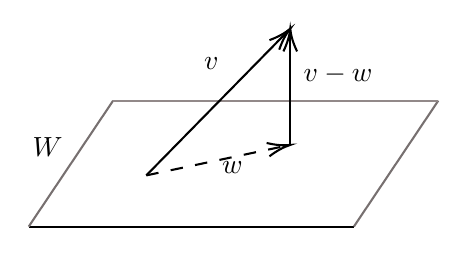
\begin{tikzpicture}[line width=0.75pt,x=0.75pt,y=0.75pt,yscale=-1,xscale=1]
%uncomment if require: \path (0,300); %set diagram left start at 0, and has height of 300

%Straight Lines [id:da5393834497664481]
\draw    (243.67,176.33) -- (400.33,176.33) ;
%Straight Lines [id:da3722628427371233]
\draw [color={rgb, 255:red, 119; green, 112; blue, 112 }  ,draw opacity=1 ]   (441,115.67) -- (400.33,176.33) ;
%Straight Lines [id:da3450034348492136]
\draw [color={rgb, 255:red, 119; green, 112; blue, 112 }  ,draw opacity=1 ]   (284.33,115.67) -- (243.67,176.33) ;
%Straight Lines [id:da008667807992642218]
\draw [color={rgb, 255:red, 146; green, 137; blue, 137 }  ,draw opacity=1 ]   (284.33,115.67) -- (441,115.67) ;
%Straight Lines [id:da7535511013685741]
\draw    (300.33,151.67) -- (368.27,82.43) ;
\draw [shift={(369.67,81)}, rotate = 134.45] [color={rgb, 255:red, 0; green, 0; blue, 0 }  ][line width=0.75]    (10.93,-3.29) .. controls (6.95,-1.4) and (3.31,-0.3) .. (0,0) .. controls (3.31,0.3) and (6.95,1.4) .. (10.93,3.29)   ;
%Straight Lines [id:da6442159524815249]
\draw  [dash pattern={on 4.5pt off 4.5pt}]  (300.33,151.67) -- (367.71,137.41) ;
\draw [shift={(369.67,137)}, rotate = 168.06] [color={rgb, 255:red, 0; green, 0; blue, 0 }  ][line width=0.75]    (10.93,-3.29) .. controls (6.95,-1.4) and (3.31,-0.3) .. (0,0) .. controls (3.31,0.3) and (6.95,1.4) .. (10.93,3.29)   ;
%Straight Lines [id:da8845013680805118]
\draw    (369.67,137) -- (369.67,83) ;
\draw [shift={(369.67,81)}, rotate = 90] [color={rgb, 255:red, 0; green, 0; blue, 0 }  ][line width=0.75]    (10.93,-3.29) .. controls (6.95,-1.4) and (3.31,-0.3) .. (0,0) .. controls (3.31,0.3) and (6.95,1.4) .. (10.93,3.29)   ;

% Text Node
\draw (326.67,93.4) node [anchor=north west][inner sep=0.75pt]    {$v$};
% Text Node
\draw (244,131.73) node [anchor=north west][inner sep=0.75pt]    {$W$};
% Text Node
\draw (335.33,143.4) node [anchor=north west][inner sep=0.75pt]    {$w$};
% Text Node
\draw (374.67,97.07) node [anchor=north west][inner sep=0.75pt]    {$v-w$};
\end{tikzpicture}
\end{center}

\begin{prop}
    For any $v \in V$, there exists a unique orthogonal projection of $v$ onto $W$, denoted $\proj_W(v)$
\end{prop}

\begin{proof}
    Let $e_1,\dots,e_k$ be an orthonormal basis of $W$, and we're looking for a specific $w = \lambda_1e_1+\cdots +\lambda_ke_k$. In particular, we require $(w-v) \perp e_i$ for all $i$, hence
    $$0=\angles{\lambda_1e_1+\cdots +\lambda_ke_k-v,e_i}=\lambda_i-\angles{v,e_i} \iff \lambda_i=\angles{v,e_i}.$$
    This gives us uniquely determined coefficients, namely
    $$\proj _W(v) = \sum_{i=1}^k\angles{v,e_i}e_i$$
\end{proof}

\begin{defn}
    The \textbf{orthogonal compliment} of a subspace $W$ is
    $$W^\perp = \{v \in V \mid \angles{v,w}=0,w \in W\}$$
\end{defn}

\begin{prop}
    $V = W \oplus W^\perp$
\end{prop}

\section{Orthogonal and Unitary Transformations}

\begin{defn}
    Let $F = \R$ (resp. $\C$), and equip $F^n$ with the standard (resp. hermitian) inner product. We say $A \in M_n(F)$ is \textbf{orthogonal} (resp. \textbf{unitary}) if its columns form an orthonormal basis of $F^n$
\end{defn}

\begin{defn}
    The \textbf{adjoint} of a matrix $A$ is defined to be $A^*:=\bar A^t$.
\end{defn}

\begin{thm}
    Let $A \in M_n(F)$. Then, TFAE
    \begin{enumerate}[(i)]
        \item $A$ is orthogonal/unitary
        \item $AA^*=A^*A=I$
        \item $A$ preserves the inner product, i.e. $\angles{Ax,Ay}=\angles{x,y}$.
        \item $A$ is a \textbf{linear isometry}, meaning it preserves distance, i.e. $d(Ax,Ay)=d(x,y)$.
    \end{enumerate}
\end{thm}

\begin{proof}
    Exercise.
\end{proof}

As usual, we can extend the notion of unitary and orthogonal matrices to linear maps.

\begin{defn}
    If $V$ is a standard (resp. hermitian) inner product space, we say $T\in \Hom(V,V)$ is orthogonal (resp. unitary) if $\angles{Tx,Ty}=\angles{x,y}$ for all $x,y \in V$. This is equivalent to $(T)_B$ being orthogonal (resp. unitary) with respect to any orthonormal basis $B$.
\end{defn}

\begin{ex}
    Let $A \in M_n(\R)$ be orthogonal, so $AA^t=I$. It's known that $\det (A) = \det (A^t)$, hence $\det (A)^2=\det (I)=1$, therefore $\det (A) = \pm 1$. We say $A$ is \textbf{orientation preserving} if $\det (A)= 1$, and $A$ is \textbf{orientation reversing} if $\det (A) = -1$.

    Now, consider the case when $A \in M_2(\R)$, letting $A = \matr{Ae_1 & Ae_2}.$ As the columns are assumed to be orthonormal, we know that if the first column is $(x,y)$, then $x^2+y^2=1$. It follows that $x = \cos \theta$ and $y = \sin \theta$ for some $\theta \in \R$. It then follows by the necessary othonormality of the columns that either
    \begin{enumerate}
        \item[(a)] $Ae_2 = \matr{- \sin \theta \\ \cos \theta}$, so $A$ is the orientation preserving rotation by $\theta$
        \item[(b)] $Ae_2=\matr{\sin \theta \\ - \cos \theta}$, so $A$ is the orientation reversing reflection about some line.
    \end{enumerate}
\end{ex}

Recall the definition of an isometry from earlier:

\begin{defn}
    An \textbf{isometry} or \textbf{rigid motion} $m: \R^n \to \R^n$ is a function that preserves distances. That is, $d(m(a),m(b)) = d(a,b)$ for all $a,b \in \R^n$.
\end{defn}

\begin{thm}
    \begin{enumerate}
        \item[(a)] An isometry $m:\R^n \to \R^n$ with $m(0)=0$ is linear. Hence, it is left multiplication by some orthogonal matrix.
        \item[(b)] Furthermore, every isometry of $\R^n$ is the composition of an orthogonal map and a translation $\tau _v$ for some $v \in \R^n$ (so $\tau_v(x)=x+v$)
    \end{enumerate}
\end{thm}


\newpage
\notechapter{Groups}
% !TEX root = ../math600-notes.tex

\section{Basics of Groups}

\begin{defn}
    A set $G$ is a \textbf{group} if it's equipped with a binary operation $\cdot :G \times G \to G$ satisfying
    \begin{enumerate}
        \item $(ab)c=a(bc)$
        \item There exists an identity element $e \in G$ such that $ae=ea = a$ for all $a \in G$.
        \item For every $a \in G$ there exists $a^{-1} \in G$ satisfying $aa^{-1}=a^{-1}a=e$.
    \end{enumerate}
\end{defn}

\begin{defn}
    A group is \textbf{abelian} if multiplication is commutative, i.e. $ab=ba$ for all $a,b \in G$. Abeliean groups are often denoted additively, and the identity is denoted by $0$.
\end{defn}

\begin{ex}
    $(\Z, +), (\Q,+)$, $(\R^\times, \cdot)$, $(\C^\times, \cdot)$ are all abelian groups.
\end{ex}

\begin{ex}
    Given a set $A$, we can define $S(A) = \{f:A \to A \mid f$ is bijective$\}$, i.e. the set of all permutations of the elements of $A$. Then, $(S(A), \circ)$ is a group under composition.
\end{ex}

\begin{defn}
    For $A = \{1,\dots,n\}$, $(S(A), \circ)$ is the \textbf{symmetric group} $S_n$
\end{defn}

Note that $S_3$ is non-abelean, and in fact is the smallest non-abelian group

\begin{ex}
    Let $F$ be a field. Then, we have various \textbf{matrix groups}. These include
    \begin{enumerate}
        \item $GL_n(F) = \{ A \in M_n(F) \mid A$ is invertible $\}$. This is called the \textbf{general linear group.}
        \item $SL_n(F) = \{ A \in GL_n(F) \mid \det A = 1\}.$. This is the \textbf{special linear group}
        \item Given any finite dimensional $F$-vector space $V$, we have the group of linear automorphisms $\Aut(V)=\{T \in \Hom(V,V) \mid T$ is invertible$\}$. By choosing a basis $\mathcal B$ of $V$, we can identify $\Aut (V) \cong GL_n(F)$.
        \item When $F=\R$, we have the \textbf{orthogonal group} $O(n) = \{ A \in GL_n(\R) \mid AA^t=I\}$. Moreover, we have the \textbf{special orthogonal group}  $SO(n)= O(n) \cap SL_n(\R)$
        \item When $F = \C$, we have the \textbf{unitary group} $U(n) = \{A \in GL_n(\C) \mid AA^*=I\}$. Moreover, we have the \textbf{special unitary group} $SU(n) = U(n) \cap SL_n(\C)$
    \end{enumerate}
\end{ex}

\begin{prop}
    If $G$ is a group, then
    \hfill
    \begin{enumerate}[(i)]
        \item The identity element of $G$ is unique
        \item Each $a \in G$ has a unique inverse $a^{-1} \in G$
        \item $(a^{-1})^{-1}=a$ for all $a \in G$
        \item $(ab)^{-1}=b^{-1}a^{-1}$ for all $a,b \in G$
    \end{enumerate}
\end{prop}

\begin{proof}

    (ii): Given $a$ with inverses $a',a''$, we have $a' = a'e = a'(a a'')=(a'a)a''=ea''=a''$
\end{proof}

\begin{prop}[Cancellation Laws]
    \begin{enumerate}[(i)]
        \item $ax=ax' \implies x=x'$
        \item $xa=x'a \implies x=x'$
    \end{enumerate}
\end{prop}

\section{Subgroups}

\begin{defn}
    A non-empty subset $H$ of a group $G$ is a \textbf{subgroup} if it's closed under the group operations multiplication and inversion.
\end{defn}

Note that this definition implies $e=aa^{-1} \in H$

\begin{lem}
    Let $H$ be a nonempty subset of a group $G$ which is finite and closed under multiplication. Then, $H$ is a subgroup of $G$.
\end{lem}

\begin{proof}
    Given $a \in H$, we must show that $a^{-1} \in H$. We have $a,a^2,\dots$ are all in $H$, and since $H$ is finite, there exists $r,s$ with $r<s$ such that $a^r=a^s$. Then, $a^{s-r}=e$, so $a(a^{s-r-1})=(a^{s-r-1})a=e$.
\end{proof}

\begin{ex}
    \begin{enumerate}
        \item Every group has the trivial subgroups $\{e\}$ and $G$
        \item Subgroups of $\Z$: Suppose $H$ is a non-zero subgroup of $\Z$. Then, let $n$ be the smallest positive number in $H$. We claim that $H = n\Z=\{ nz \mid z \in \Z\}$.
    \end{enumerate}
    \begin{proof}
        Since $n \in H$ and $H$ is closed under the group operations, the entire subgroup $n\Z \subset H$. Conversely, if $a \in H$, we may divide $a$ by $n$: $a=kn+r$ with $0 \leq r <n$. Then, $r = a-kn\in H$, so by minimality of $n$, we must have $r = 0$. Hence, every $a \in H$ is a multiple of $n$.
    \end{proof}
\end{ex}

\textbf{Application:} Given $a,b \in \Z$ both positive, let $a\Z + b\Z$ be the subgroup of $\Z$ generated by $\{a,b\}$. That is, $a\Z + b\Z = \{ax+by \mid x,y \in \Z\}$. Since this is a nonzero subgroup, we must have that $a\Z + b\Z = d\Z$ for some $d \in \Z^+$. We claim that $d=\gcd(a,b)$.

\begin{proof}
    Indeed, $d \mid a$ since $a=a\cdot 1 + b\cdot 0 \in d\Z$, hence $a = dk$ for some $k \in \Z$. Similarly, $d \mid b$.

    Now, if $c \mid a, c \mid d$, then we must have $c \mid d$, since $d \in a\Z + b\Z$, so $d=ax+by$.
\end{proof}

\begin{defn}
    If $G$ is any group and $a \in G$, we can consider the subgroup \textbf{generated} by $a$. Let $\langle a \rangle = \{a^i : i \in \Z  \}$. If there exists some $a \in G$ such that $G = \langle a \rangle$, we say that $G$ is \textbf{cyclic}.
\end{defn}

\begin{ex}
    For cyclic groups, there are two cases:
    \begin{enumerate}
        \item If all powers $a^i$, $i \in \Z$ are distinct, then $G$ is an infinite cyclic group
        \item If $a^r=a^s$ with $r<s$, then $a^{s-r}=1$. Hence $a^n = 1$ for some smallest positive integer $n$, and so $\langle a \rangle = \{1,a,a^2,\dots,a^{n-1}\}$. We in some cases call this group $C_n$. Note that $C_n$ is realized by the group of $n$'th roots of unity in $\C$, which we denote $\mu_n = \{z \in \C: z^n=1\} = \{e^{2\pi i k/n} \mid k=0,1,\dots,n-1\}$
    \end{enumerate}
\end{ex}

\begin{defn}
    The \textbf{order} of a finite group $G$, denoted $|G|$ or $o(G)$, is the number of elements in $G$. The order $o(a)$ of an element $a \in G$ is the order of the cyclic subgroup $\langle a \rangle$. So, $o(a) = \min \{k \geq 1 \mid a^k=e\}$.
\end{defn}

\begin{defn}
    Let $G$ be a group, $W \subset G$ be a subset. Then, the \textbf{subgroup generated by the subset} $W$, denoted $\langle W \rangle$, is the smallest subgroup of $G$ containing $W$. Concretely, it consists of all products of elements of $W$ and their inverses.
\end{defn}

\begin{defn}
    The \textbf{Klein group} $V$ is the smallest non-cyclic group. It is realized as a subgroup of $GL_2(\R)$ by $V=\left \{ \matr{ \pm1 & 0 \\ 0 & \pm 1} \right \}$. Note that any $2$ non-identity element in $V$ generate $V$.
\end{defn}

\begin{defn}
    The group $GL_n(F)$ has the \textbf{Borel subgroup} $B$ consisting of all upper triangular matrices.
\end{defn}

\section{Cosets and Lagrange's Theorem}

Fun fact: Lagrange invented his theorem before groups were invented

\begin{defn}
    Given $H \leq G$ ("$H$ is a subgroup of $G$"), we define an equivalence relation $x \sim y \iff x^{-1}y \in H$. We say that $x$ \textbf{conguent} to $y$ modulo $H$, and write $x \equiv y \pmod H$

    The equivalence class of $x$ is the (left) \textbf{coset} of $x$, i.e. the set $[x] = \{y \in G: x \sim y\} = \{y \mid x^{-1}y=h \in H\} = \{xh \mid h \in H\}=xH$.
\end{defn}

\begin{notebox*}
    We could have used $xy^{-1}\in H$ in the above definition, and this leads to the right cosets $Hx$
\end{notebox*}

\begin{prop}
    The inversion map $x \mapsto x^{-1}$ gives a $1-1$ correspondence between left and right $H$-cosets, since $H^{-1}=\{h^{-1}\mid h \in H\} = H$, hence $(xH)^{-1}=Hx^{-1}$. We'll use left $H$-cosets. The two notions coincide for abelian groups
\end{prop}

\begin{ex}
    If $G = (\Z, +),H=n\Z$, then $x \equiv y \pmod H \iff x\equiv y \pmod n$. The cosests are $n\Z,1+n\Z,\dots,(n-1)+n\Z$.
\end{ex}

\begin{prop}
    There is a $1-1$ correspondence between any two (left) $H$-cosets. Furthermore, the cosets form a partition of $G$.
\end{prop}

\begin{proof}
    The cosets partition $G$ because they are equivalence classes. Given any two cosets $aH$ and $bH$, the map $f:aH \to bH$ sending $ah \mapsto bh$ is $1-1$ and onto by the cancellation law.
\end{proof}

\begin{thm}[Lagrange's Theorem]
    Let $G$ be a finite group, and $H \leq G$. Then, $|H|$ divides $|G|$
\end{thm}

\begin{proof}
    If $k$ is the number of left $H$-cosets, then $G$ is partitioned into $k$ subsets, each with $|H|$ elements. Hence, $|G| = |H|\cdot k$
\end{proof}

\begin{defn}
    The number of left (or right) $H$-cosets is the \textbf{index} of the subgroup $H$ in $G$, denoted $|G:H|$. Hence, $|G| = |H| \cdot |G:H|$
\end{defn}

\begin{cor}
    \begin{enumerate}
        \item[(a)] If $G$ is a finite group and $a \in G$, then $o(a) \mid o(G)$.
        \item[(b)] If $|G|<\infty$ and $a \in G$, then $a^{|G|}=e$.
        \item[(c)] If $G$ is a finite group with prime order, then $G$ is cyclic.
    \end{enumerate}
\end{cor}

\begin{defn}[The Quotient Set]
    Given any two subsets $A,B$ of a group $G$, we define $AB=\{ab \mid a\in A,b \in B\}$. Let $G/H$ denote the set of all left $H$-cosets of $G$. We want to make this set into a group, with multiplication of cosets.
\end{defn}

Suppose this were the case. Then, for any $g \in G$, $A:=gHg^{-1}H$ must equal another $H$-coset. Clearly, $e \in A$, so as the $H$-cosets partition the group $G$, we must have $A = H$. That is, $gHg^{-1}H=H\implies ghg^{-1}\in H$ for all $g\in G,h \in H$.

\begin{defn}[Normal Subgroups]
    A subgroup $N \leq G$ is a \textbf{normal subgroup} if for each $n \in N$ and $g \in G$, $gng^{-1}\in N$. Equivalently, $gNg^{-1}\subset N$
\end{defn}

\begin{prop}
    The following are equivalent, for $N \leq G$
    \begin{enumerate}
        \item $N$ is a normal subgroup of $G$, denoted $N \unlhd G$
        \item $gNg^{-1}=N$ for all $g \in G$
        \item Every left coset of $N$ is also a right coset of $N$ in $G$.
    \end{enumerate}
\end{prop}

\begin{proof}

    (i) $\implies$ (ii): Assume $gNg^{-1} \subset N$. Then, $N=g(g^{-1}Ng)g^{-1}\subset gNg^{-1}$.

    (ii) $\implies$ (iii): $gNg^{-1}=N \iff gN=Ng$.

    (iii) $\implies$ (i): Given any $g \in G$, we have $gN=Nx$ for some $x \in G$. We must therefore have $Nx=Ng$ since $g\in gN = Nx$ and $g \in Ng$. Hence, we get (i)
\end{proof}

We can therefore define a group structure on $G/N$ when $N$ is normal in $G$, setting $(aN)(bN)=a(Nb)N=a(bN)N=abN$.

\begin{defn}
    The above defines the \textbf{quotient group} $G/N$
\end{defn}

\begin{ex}
    If $G$ is abelian, then every subgroup of $G$ is normal, so we always get a quotient group.
\end{ex}

\begin{ex}[Modular arithmetic]
    Let $G=\Z$, $H=n\Z$. So, $\Z/n\Z=\{\bar 0,\dots,\overline{n-1}\}$, where $\bar x :=x \pmod n$.
\end{ex}

\begin{defn}
    $(\Z / n\Z)^\times$ consists of the multiplicatively invertible elements in $\Z/n\Z \setminus\{0\}$, which are exactly the equivalence classes coprime to $n$. This makes $(\Z/n\Z)^\times$ a multiplicative group with order $\varphi (n)$.
\end{defn}

\begin{notebox*}[Fact]
    Normal subgroups are exactly the kernels of group homomorphisms.
\end{notebox*}

\begin{defn}[Homomorphisms and Isomorphisms]
    A map $\varphi:G \to G'$ between two groups is a \textbf{homomorphism} of groups if it preserves the group operations: $\varphi(ab)=\varphi(a)\varphi(b)$ for all $a,b \in G$. Furthermore, if $\varphi$ is bijective, we say it is an \textbf{isomorphism}.
\end{defn}

\begin{defn}[$\Hom(G,G')$ and $\Aut(G)$]
    We write $\Hom(G,G') :=$ the set of all homomorphisms $G \to G'$. An isomorphism $G\to G$ is called an \textbf{automorphism} of $G$, and these form a group $\Aut(G)$
\end{defn}

\begin{ex}
    For any homomorphism $\varphi :G \to G'$, $\varphi (e)=e'$ and $\varphi(x)^{-1}=\varphi(x^{-1})$.
\end{ex}

\begin{defn}
    The \textbf{kernel} of $\varphi$ is the set of $g \in G$ such that $\varphi (g)=e'$, and the image is $\Img \varphi=\varphi(G)$
\end{defn}

\begin{notebox*}[Check]
    $\ker \varphi$ is always a normal subgroup of $G$.
\end{notebox*}

\begin{thm}[First Isomorphism Theorem]
    For any homomorphism $\varphi:G \to G'$ of groups, $G/\ker \varphi \cong \Img \varphi$, with the map $g\ker \varphi \mapsto \varphi(g)$.
\end{thm}

\begin{proof}
    Same as for vector spaces.
\end{proof}

\begin{ex}
    \begin{enumerate}
        \item For any field $F$, $SL_n(F)=\ker (\det :GL_n(F) \to F^*)$, so we have a normal subgroup of $GL_n(F)$. Furthermore, $GL_n(F) / SL_n(F) \cong (F^*,\cdot)$
        \item If $N \unlhd G$, then we have a projection map $\pi:G \to G/N$ by $g \mapsto gN$, and $N = \ker \varphi$. This helps show how normals subgroups are equivalent to the kernels of homomorphisms
        \item Consider $S^1=\{z \in \C : |z| =1\} \leq \C^\times$, both of which are groups under multiplication. We have $\C^\times \to \R_{>0}$ by $z \mapsto |z|$, and $\ker \varphi = S^1$. So, $\C^\times / S^1 \cong \R_{>0}$
    \end{enumerate}
\end{ex}

\begin{thm}[Universal Property of Quotient Construction]
    % https://q.uiver.app/#q=WzAsMyxbMiwwLCJHIl0sWzQsMiwiRy9OIl0sWzAsMiwiRyciXSxbMCwxLCJcXHBpIl0sWzAsMiwiZiIsMl0sWzEsMiwiXFxleGlzdHMgISBcXHRpbGRlIGYiLDAseyJzdHlsZSI6eyJib2R5Ijp7Im5hbWUiOiJkYXNoZWQifX19XV0=
    Given any group hom $f :G \to G'$ such that $N \subset \ker f$, there exists a unique map $\tilde f:G/N \to G'$ s.t. $\tilde f \circ \pi = f$. That is, the following diagram commutes.
\end{thm}
\[\begin{tikzcd}
	&& G \\
	\\
	{G'} &&&& {G/N}
	\arrow["f"', from=1-3, to=3-1]
	\arrow["\pi", from=1-3, to=3-5]
	\arrow["{\exists ! \tilde f}", dashed, from=3-5, to=3-1]
\end{tikzcd}\]

\section{Products of Groups}

\begin{defn}[External Direct Products]
    Given two groups $G_1,G_2$, we define $G_1 \times G_2$ as a cartesian product of the sets, with the group operation defined component-wise.
\end{defn}

\begin{notebox*}
    $\bar G_1 := G_1 \times \{e_2\}$, and $\bar G_2:= \{e_1\} \times G_2$ are normal subgroups of $G_1 \times G_2$.
\end{notebox*}

\begin{notebox*}[Question]
    Given two subgroups $H$ and $K$ of a group $G$, when is $HK$ a subgroup?
\end{notebox*}

\begin{prop}
    $HK$ is a subgroup of $G \iff HK = KH$
\end{prop}
\begin{proof}
    If $HK \leq G$, then $HK=(HK)^{-1}=K^{-1}H^{-1}=KH$. Now, suppose $HK=KH$. Observe
    $$(h_1k_1)(h_2k_2)=h_1(k_1h_2)k_2=h_1(h_3k_3)k_2=h_4k_4$$
    $$(h_1k_1)^{-1}=k_1^{-1}h_1^{-1}=h'k'.$$
    So, $HK$ is a group
\end{proof}

\begin{cor}
    If $H,K \leq G$ and $H$ or $K$ is normal in $G$, then $HK \leq G$
\end{cor}

\begin{proof}
    Say $H \lhd G$. Then, $HK= \cup Hk=\cup kH=KH$. So, $HK$ is a subgroup by the above proposition
\end{proof}

\begin{defn}[Internal Direct Products]
    Let $H$,$K$ be subgroups of $G$. Then, we say $G$ is the internal direct product of $H$ and $K$ if
    \begin{enumerate}
        \item[(i)] $H$ and $K$ are both normal
        \item[(ii)] $G=HK$
        \item[(iii)] Given any $g \in G$, we can write $g=hk$ for $h \in H$ and $k \in K$ in a unique way
    \end{enumerate}
    This definition generalizes to more than $2$ subgroups.
\end{defn}

\begin{lem}
    Suppose $G=N_1\cdots N_k$ is an internal direct product of its subgroups $N_i \lhd G$. Then, for each $i \neq j$, we have $N_i \cap N_j = \brax{e}$, and for $a \in N_i, b \in N_j$, $ab=ba$.
\end{lem}

\begin{proof}
    Suppose $x \in N_i \cap N_j$. Then, $x=e\cdots e \cdot x_i\cdot e \cdots e=e \cdots e \cdot x_j \cdot e \cdots e$, we by uniqueness of representation, $x=e$. If $a \in N_i$, $b \in N_j$, consider the commutator $[a,b] := aba^{-1}b^{-1}$. We then have $[a,b]=(aba^{-1})b^{-1}=a(ba^{-1}b^{-1})$. Observe $aba^{-1} \in N_j$ and $ba^{-1}b^{-1} \in N_i$ by normality. So, the commutator lies in $N_i \cap N_j = \{e\}$. Thus, $ab=ba$.
\end{proof}

\begin{rmk}
    If $N_1,\dots,N_k$ are normal subgroups of $G$, we need a stronger condition than $N_i \cap N_j = \{e\}$ for $i \neq j$ to ensure that the product is a direct product. Namely, we need $N_i \cap(N_1\cdots N_{i-1}N_{i+1}\cdots N_k)=\{e\}$.
\end{rmk}

\begin{thm}
    Suppose $G$ is the internal direct product $G=N_1\cdots N_k$. Then, $G$ is isomorphic to the external direct product $N_1 \times \cdots \times N_k$.
\end{thm}

\begin{proof}
    The map $\varphi :G\to N_1 \times \cdots \times N_k$ sending $x_1\cdots x_k \mapsto (x_1,x_2,\dots,x_k)$ is well defined by uniqueness. Furthermore, $\varphi$ is clearly bijective. Moreover, $\varphi((x_1\cdots x_k)(y_1\cdots y_k))=\varphi(x_1y_1\cdots x_ky_k)$ by the previous lemma. This maps to
    $$(x_1y_1,\dots,x_ky_k)=(x_1,\dots,x_k)(y_1,\dots,y_k)=\varphi(x_1\cdots x_k)\varphi (y_1\cdots y_k)$$
\end{proof}

Because of this theorem we do not distinguish between internal and external direct products.

\begin{ex}[On Homework]
    If $C_n$ is cyclic of order $n$, show that if $\gcd (m,n)=1$, then $C_m \times C_n \cong C_{mn}$.
\end{ex}

\begin{thm}[Second Isomorphism Theorem]
    If $M$ and $N$ are subgroups of $G$ with $N \lhd G$, then there is a natural isomorphism $MN/N\cong M/M\cap N$
\end{thm}

\begin{proof}
    Let $\varphi:M \to MN/N$ map $m \mapsto mN$. Then, $\varphi$ is clearly surjective, and
    $$\ker \varphi =\{ m \in M \mid m \in N\} = M \cap N.$$
    Thus, the first isomorphism theorem gives $M /M \cap N \cong MN/N$.
\end{proof}

\begin{cor}
    If $M$ and $N$ are as above and are both finite subgroups, then $|MN| = \frac{|M||N|}{|M \cap N|}$
\end{cor}

\section{Inner Automorphisms of a Group}

Let $G = GL_n(F)$. Then, for a fixed $P \in G$, we have the map $A \mapsto PAP^{-1}$, an automorphism. We want to generalize this.

\begin{defn}
    Let $G$ be a group, and $g\in G.$ We define $T_g:G\to G$ by $T_g(x)=gxg^{-1}$. Then, $T_g \in \Aut G$, i.e. it's an isomorphism from $G$ to itself. We call $T_g$ the \textbf{inner automorphism given by $g$}.
\end{defn}

\begin{notebox*}
    $T_g \circ T_h(x)=g(hxh^{-1})g^{-1}=(gh)x(gh)^{-1}=T_{gh}(x)$. So, $T_g \circ T_h = T_{gh}$.
\end{notebox*}

\begin{defn}
    Let $\mathcal I(G)$ be the group of all inner automorphisms of $G$, under composition. We then have a morphism $\psi :G \to \mathcal I(G)$ sending $g \mapsto T_g$.
\end{defn}

What is the kernel of $\psi$?

$\ker \psi = \{g \in G \mid T_g(x) = x\}=\{g \in G\mid gx=xg,x\in G\}=Z(G)$, the \textbf{center} of $G$. Thus,

\begin{prop}
    As $\Img \psi = \mathcal I(G)$, we have $\mathcal I(G) \cong G/Z(G)$.
\end{prop}

\begin{ex}
    For $G = GL_n(F)$, we showed in HW 1 that the center of $Z(G) =\{\lambda I_n:\lambda \in F^\times\}\cong F^\times$. So, $\mathcal I(GL_n(F)) \cong GL_n(F)/F^\times=: PGL_n(F)$. We can think of $GL_n(F)$ as linear automorphisms on $F^n$, and by analogy $PGL_n(F)$ are algebraic automorphisms of $P(F^n)=\mathbb P^{n-1}_F$, which is $n-1$ dimensional projective space.
\end{ex}

\section{Symmetry}

Let $M_n$ be the group of all isometries or rigid motions $\R^n \to \R^n$.

\begin{notebox*}[Recall]
    Any $m \in M_n$ has representation as $m=\tau _v \circ \rho$, where $\tau _v(x) = x+v$ is a translation by $v$, and $\rho \in O(n)$.
\end{notebox*}

\begin{defn}
    Let $F \subset \R^n$ be a subset. A \textbf{symmetry} of $F$ is a rigid motion $m$ with $m(F)=F$. The set of all symmetries of $F$ form a subgroup of $M_n$, which is the group of symmetries of $F$.
\end{defn}

\begin{notebox*}[Goal]
    Find all possible finite groups of symmetry of plane figures.
\end{notebox*}

\begin{thm}
    Let $G$ be a finite subgroup of $M_n$. Then, there exists $x \in \R^n$ fixed by all $g \in G$, i.e. $g(x)=x$ for all $g \in G$.
\end{thm}

\begin{proof}
    Given any point $s \in \R^n$, consider the orbit $\mathcal O_s$ under the action of $G$. That is, $\mathcal O_s:=\{g(s)\mid g \in G\}$. Any $g \in G$ permutes the set $\mathcal O_s$, since $\mathcal O_s$ is a finite set and $g$ is injective on $\R^n$, hence is injective on $\mathcal O_s$.
    \begin{lem}
        Let $S:=\{s_1,\dots,s_n\}$ be a finite set in $\R^m$. Let $p:= \frac 1n(s_1+\cdots +s_n)$ be the \textbf{center of gravity} of $S$. Then, if $s_i'=g(s_i)$ for $g \in M_n$, and $g(p)=p'$, then $p'=\frac 1n(s_1'+\cdots +s_n')$. That is, rigid motions send centers of gravity to centers of gravity.
    \end{lem}
    \begin{proof}
        Since $g = \tau_v \circ \rho$, it suffices to consider the 2 cases:
        \begin{enumerate}
            \item[(i)] $g=\rho$ is linear. Then, $g(p)=g(\frac 1n \sum s_i)=\frac 1n \sum s_i'=p'$.
            \item[(ii)] $g = \tau _v$. Then, $\tau_v(s_i)=s_i+v$, so $\tau _v(p)=p+v=p'$.
        \end{enumerate}
    \end{proof}
    Now, to prove the theorem, notice that the lemma implies any $g \in G$ fixes the center of gravity of $\mathcal O_s$.
\end{proof}

\section{\texorpdfstring{Finite Subgroups of $\mathcal O(2)$}{Finite Subgroups of O(2)}}
By the theorem, any finite subgroup of $M_2$ has a fixed point $o$. By choosing coordinates so that $o$ is the origin, we reduce to $G \leq O(2)$.

\begin{thm}[][label=thm:finite-o2]
    If $G$ is a subgroup of $O(2)$, and $|G| < \infty$, then
    \begin{enumerate}
        \item[(i)] $G= C_n$, the cyclic group of order $n$ generated by the rotation $\rho _\theta$, where $\theta=2\pi /n$
        \item[(ii)] $G=D_n$, the dihedral group of order $2n$, generated by a rotation $\rho_ \theta$ for $\theta = 2\pi /n$, and a reflection $r$ about the line through the origin $0$. We can choose coordinates so that $r$ is a reflection $\matr{1 & 0 \\ 0 & -1}$ about the $x$-axis.
    \end{enumerate}
\end{thm}

\begin{cor}
    If $G$ is a finite subgroup of $M_2$, then for a suitable choice of coordinates, $G$ becomes one of the groups $C_n$ or $D_n$, where $C_n$ is generated by $\rho _{2\pi/n}$, and $D_n$ by $\rho_{2\pi / n}$ and $r$. When $n \geq 3$, $D_n$ is the group of symmetries of an $n$ sided regular polygon.
\end{cor}

\begin{ex}
    \begin{enumerate}
        \item $C_1 = \{1\}, D_1=\{1,r\},C_2=\{1, \rho _ \pi\}, D_2 = \{1, \rho_\pi, r, \rho _\pi \circ r\} \cong V_4$
    \end{enumerate}
\end{ex}

\begin{prop}
    $D_n$ is generated by two elements $x$ and $y$ satisfying the relations $x^n=1$, $y^2=1$, and $yx=x^{-1}y$. The elements of $D_n$ are exactly $\{1,x,x^2,\dots,x^{n-1},xy,x^2y,\dots,x^{n-1}y\}$, so $|D_n| = 2n$.
\end{prop}

\begin{proof}
    We let $x = \rho _{2 \pi /n}$ and $y = r$. Clearly, $x,y$ satisfy the given relations...
\end{proof}

\begin{notebox*}[Exercise]
    If $x=\case{1 \to 3 \\ 2 \to 1 \\ 3 \to 2}$ and $y = \case{1 \to 2 \\ 2 \to 1 \\ 3 \to 3}$ are in $S_3$, check that $x^3=1,y^2=1$, and $yx=x^{-1}y$, hence $D_3 \cong S_3$
\end{notebox*}

\begin{proof}
    Proof of \Cref{thm:finite-o2}. Let $G \leq O(2),|G| < \infty $.

    Case $1$: $G \leq SO(2)$, i.e all elements in $G$ are rotations. If $G = \{1\}$, we're ok, so assume $G$ is non-trivial. Let $\theta = \min \{\alpha >0 \mid \rho _\alpha \in G\}$, which exists as $G$ is finite. Then, $G = \langle \rho _\theta \rangle$. [Indeed, if $\rho _\alpha \in G$, then $\alpha + n \theta + \beta$, where $0 \leq \beta < \theta$. So, $\rho _\beta=\rho _\alpha (\rho _\theta)^{-n}\in G \implies \beta =0$ by definition of $\theta$.] Thus, $G$ is a finite cyclic group $C_n$.

    Case $2$: $G$ contains an element of the form $\rho _\theta \circ r$. Since $\rho _\theta \circ r=\matr{\cos \theta & \sin \theta \\ \sin \theta & -\cos \theta}$ has a square of $1$, it must be a reflection as it is orthogonal. In fact, check that $\rho _\theta \circ r \matr{\cos (\theta /2)\\ \sin (\theta /2)} =\matr{\cos (\theta /2)\\ \sin (\theta /2)}$, so $\rho _\theta r$ is a reflection about the line $\langle \matr{\cos (\theta /2)\\ \sin (\theta /2)} \rangle$. Adjusting coordinates if necessary, we may assume $r \in G$. Let $H:= G \cap SO(2)$, the subgroup of rotations in $G$. By case $1$, we get that $H$ is cyclic, generated by $\rho _\theta$ where $\theta = 2\pi /n$. Hence $G$ contains all products $\rho _\theta^ir^j$ for $0 \leq i < n$, $0 \leq j <2$, so $D_n \subset G$. Now, if $x$ is an arbitrary orientation reversing element of $G$, then $xr \in SO(2) \cap G = H$, so $x \in H_r \subset D_n$. Thus, $G=D_n$.
\end{proof}

\begin{thm}
    Every finite subgroup of $SO(3)$ is one of the following:
    \begin{enumerate}
        \item The cyclic group $C_n$ of rotations by multiples of $2\pi /n$ about a line through the origin.
        \item The dihedral group $D_n$
        \item The tetrahedral group of $12$ rotations carrying a regular tetrahedron to itself. ($A_4$)
        \item The octahedral group of $24$ rotations of a cube or regular octahedron ($S_4$)
        \item The icosahedral group of $60$ rotations of a regular dodecahedron or icosahedron. ($A_5$)
    \end{enumerate}
\end{thm}

In every dimension, the tetrahedron generalizes to the simplex, the cube generalizes to the hypercube, and the regular octahedron generalizes to the convex hull $\langle \pm e_1,\dots, \pm e_n\rangle$.

\begin{rmk}
    The tetrahedron, cube, and octahedron have analogues forms in all dimensions. The only other regular polytopes are
    \begin{enumerate}
        \item Dimension $3$: case (5)
        \item Dimension $4$: (Schläfli, 1842) The $24$-cell, $120$-cell, $600$-cell, bounded by $24$ octahedra, $120$ dodecahedra, and $600$ tetrahedra respectively.
        \item That's it lol
    \end{enumerate}
\end{rmk}

\section{Group Actions}

\begin{defn}[Group Actions]
    Let $G$ be a group and $X$ be a set. We say that $G$ \textbf{acts on} $X$ (on the left) if there exists a map $G \times X \to X$, given by $(g,x) \mapsto g\cdot x$, satisfying
    \begin{enumerate}
        \item[(i)] $e\cdot x=x$ for all $x \in X$
        \item[(ii)] $(g_1g_2)\cdot x=g_1\cdot(g_2\cdot x)$ for all $g_1,g_2\in G,x \in X$.
    \end{enumerate}
    We also say that $X$ is a $G$-set.
\end{defn}

\begin{ex}
    \begin{enumerate}
        \item The group $M_2$ of rigid motions of the plane $\R^2$ acts on the set of points, the set of lines, the set of triangles, etc.
        \item Any group $G$ acts on itself by
        \begin{itemize}
            \item Left multiplication
            \item Conjugation (inner automorphisms)
        \end{itemize}
        \item If $H$ is a subgroup of $G$, then $G$ acts naturally on $G/H$ by $g\cdot(xH)=gxH$.
        \item For any set $X$, $S(X)$ acts on $X$.
        \item The group $G$ of rotational symmetries of the cube acts on the set of (1) faces of the cube; (2) edges of the cube; (3) vertices of the cube.
        \item Suppose $X$ is a connected manifold with universal covering space $p:\tilde X \to X$. Fix a base point $x \in X$. Then the fundamental group $\pi_1(x)$ acts on $p^{-1}(x)$. For example, $p: \R \to S^1$, $\theta \mapsto e^{2\pi i \theta} \dots$
        \item Suppose $K$ is a finite field extension of $\Q$. We have a ring of "integers" $\mathcal O _K$ in $K$ such that $\mathcal O_K \cap \Q = \Z$. Any prime ideal $\mathcal P$ of $\mathcal O_K$ lies above a rational prime $p \in \Z$ if $\mathcal P \cap \Z = p\Z$. For any $p \in \Z$, there exist finitely many prime ideals $P_1,\dots,P_r$ above $p$. If $K/\Q$ is a Galois extension, then the Galois group $G$ acts transitively on the set of these $r$ prime ideals. For example, $K=\Q ( \zeta _n)$, and then $\mathcal O_K=\Z [\zeta _n]$, and the Galois group if $G = (\Z/n\Z)^\times$.
    \end{enumerate}
\end{ex}

\begin{prop}[Permutation Representations]
    Let $G$ be a group and $X$ be a set. There is a $1-1$ correspondence between actions of $G$ on $X$ and group homomorphisms $G \to S(X)$. Such homomorphisms are called \textbf{permutation representations} of $G$
\end{prop}

\begin{proof}
    If $G$ acts on $X$, then for any $g \in G$, define $\eta_g \in S(X)$ by $\eta_g(x):=g\cdot x$. Check that $\eta_g$ is a bijection and the map $g \mapsto \eta_g$ is a group homomorphism $G \to S(X)$. Conversely, given a group homomorphism $\varphi :G \to S(X)$, we define an action of $G$ on $X$ by $g \cdot x = \varphi(g)(x)$. Check that these two processes are inverse to each other.
\end{proof}

\begin{defn}
    A $G$-action is faithful if the corresponding map $G \to S(X)$ is injective. This means that $g\cdot x =x\:\: \forall x \in X \implies g=e$.
\end{defn}

\begin{thm}[Cayley's Theorem]
    Every group $G$ is isomorphic to a subgroup of $S(G)$. In particular, if $|G| = n$, then $G \leq S_n$
\end{thm}

\begin{proof}
    Note that the action of $G$ on itself by left multiplication is faithful, so we get an injection $G \hookrightarrow S(G)$.
\end{proof}

\begin{defn}
    Let $X$ be a $G$-set. Then, for any $x \in X$, the \textbf{orbit} of $x$, denoted $\mathcal O_x$, is the set $\mathcal O_x=\{gx \mid g \in G\}$. $\mathcal O_x$ is itself a $G$-set. Furthermore, the orbits for a $G$-action are equivalence classes for the equivalence relation $x \sim y \iff x=gy$ for some $g \in G$.
\end{defn}

\begin{prop}
    The orbits of $X$ partition the set $X$. Every $x \in X$ lies in exactly one orbit, namely $\mathcal O_x$.
\end{prop}

\begin{defn}
    If $X$ consists of just one orbit, we say that $G$ acts transitively on $X$. So, this occurs if and only if $\forall x,y \in X,\exists g\in G$ such that $y=g \cdot x$.
\end{defn}

\begin{defn}
    If $x,y \in X$ lie in the same $G$-orbit, we often say they are \textbf{conjugates} under the $G$-action.
\end{defn}

\begin{defn}
    For $x \in X$, the \textbf{stabilizer} $G_x$ of $x$ is the subgroup $G_x := \{ g \in G\mid g \cdot x = x\}$
\end{defn}

\begin{thm}
    \begin{enumerate}[(a)]
        \item If $X$ is a transitive $G$-set and $x \in X$, then there is a natural bijection $\varphi:G/G_x \to X$ which maps $gG_x \mapsto g\cdot x$, which is compatible with the $G$-action, that is $\varphi (gC)=g \cdot \varphi(C)$ for every coset $C$. Thus, $G/G_x$ and $X$ are isomorphic as $G$-sets. In particular for an arbitrary $G$-action, we have $G/G_x \cong \mathcal O_x$ for any $x \in X$.
        \item If $X$ is any $G$-set, then $G_{gx}=gG_xg^{-1}$ for all $g\in G,x\in X$. So, the stabilizer subgroups of points belonging to the same $G$-orbit are conjugate.
    \end{enumerate}
\end{thm}

\begin{proof}
    \hfill
    \begin{enumerate}
        \item[(a)]
    \end{enumerate}
    $gG_x = g'G_x \iff g^{-1}g' \in G_x \iff g^{-1}g'(x)=x \iff g \cdot x = g'\cdot x$. This shows $\varphi$ is well defined and injective. If $y \in X$, there exists $g \in G$ such that $y=g\cdot x$ by transitivity, so $y = \varphi(g\cdot G_x)$, thus $\varphi$ is surjective. Finally, it's easy to check that $\varphi$ respects the $G$-action.
    \begin{enumerate}
        \item[(b)]
    \end{enumerate}
    $G_{gx}=\{u \in G \mid ugx = gx\} =\{ u \in G \mid (g^{-1}ug)x=x\}=\{ u \in G\mid g^{-1}ug \in G_x\} = gG_xg^{-1}$
\end{proof}

\begin{ex}
    \begin{enumerate}
        \item Let $M$ be the group of rigid motions of $\R^2$. If $p \in \R^2$ is any point, then $M_p =M_{\tau _p(0)}=\tau _pM_0\tau_p^{-1}=\tau _p O(2) \tau_p^{-1}$, by part (b)
        \item \textbf{(Exercise)} Let $h = \{ z \in \C \mid Im(z) >0\}$ be the upper half plane in $\C$, and $G = SL_2(\R)$. For $g \in \matr{a & b \\ c & d} \in G$, we let $g\cdot z =\frac{az+b}{cz+d}$. Check that this defines a transitive $G$-action on $h$. The stablizer subgroup of $i=\sqrt{-1}$ is $K:=G_i:=\brax{\matr{\cos \theta & -\sin \theta \\ \sin \theta & \cos \theta}\mid \theta \in \R}$. Therefore, $h \equiv SL_2(\R)/K$
    \end{enumerate}
\end{ex}

\begin{cor}
    For any $G$-action on a finite set $X$, we have the counting formulas:
    $$|X|=\sum_{\text{orbits}}|\mathcal O_x|= \sum|G:G_x|,$$
    where the sum is over distinct orbits, and
    $$|\mathcal O_x| = |G| / |G_x| \iff |G| = |\mathcal O_x| \cdot |G_x|,\forall x \in X$$
\end{cor}

\begin{ex}
    \begin{enumerate}
        \item A group is \textbf{simple} if its only normal subgroups are $\{e\}$ and itself. If $H$ is any proper subgroup of a simple group $G$, we get an injection $G \hookrightarrow S_k$, where $k = |G:H|$ (Just consider the $G$-action on the coset space $G/H \ \iff$ a map $G \to S(G/H)$)
        \item \textbf{Check:} If $H$ and $K$ are subgroups of $G$, then the $G$-sets $G/H$ and $G/K$ are isomorphic if and only if $H$ and $K$ are conjugate subgroups of $G$.
        \item Suppose $G$ is a finite group and $H$ and $K$ are two subgroups of $G$. We compute $|HK|$. Consider $X := G/K$ and consider the action of $H$ on $X$ by left multiplication. Then, the orbit of $K$ in $G/K$ under the $H$-action is $HK$. Therefore, $|HK| = |K| \cdot$(\# of $H$-cosets that lie in this orbit). The stabilizer $H_K$ of the coset $K$ is $H \cap K$, hence the orbit in question includes $|H:H \cap K|$ cosets of $K$. Thus, $|HK| = \frac{|H| \cdot |K|}{|H \cap K|}$
    \end{enumerate}
\end{ex}

\section{\texorpdfstring{Conjugacy Classes in $G$; The Class Equation}{Conjugacy Classes in G; The Class Equation}}
Recall the conjugation action of a group $G$ on itself is defined by $g \cdot x = gxg^{-1}$.
\begin{defn}
    The stabilizer of an element $x \in G$ under the action of conjugation is called the \textbf{centralizer} of $x$, denoted $Z(x)$. That is, $Z(x)=\{ g \in G \mid gx=xg\}$.
\end{defn}

\begin{defn}
    The orbit $\mathcal O _x$ of $x$ under the $G$-action is the \textbf{conjugacy class} $C_x=\{ y \in G \mid y= gxg^{-1}$ for some $g \in G \}$
\end{defn}

\begin{prop}[The Class Equation]
    By the counting formula, $|G| = |Z(x)| \cdot |C_x|$, so $|C_x| = |G:Z(x)|$

    We also have the \textbf{class equation}: let $x_1,\dots,x_n$ be all the representatives of distinct conjugacy classes, then
    $$|G| = \sum_{i=1}^n|C_{x_i}|=\sum_{i=1}^n|G:Z(x_i)|.$$
    Furthermore, any element in the center of $G$ only has itself in the orbit. Therefore, we can let $g_1,\dots,g_m$ be all representatives of non-central conjugacy classes, and then
    $$|G|=|Z(G)|+\sum_{i=1}^m|G:Z(g_i)|$$
    Note by assumption that $|G:Z(g_i)|\geq 2$.
\end{prop}

\begin{rmk}
    All the integers on the right hand side of the class equation divide $|G|$, and $|Z(G)| \geq 1$.
\end{rmk}

\begin{ex}
    $G= D_3$ has conjugacy classes $\{1\},\{r,r^2\},\{s,sr,sr^2\}$. The class equation is $6 = 1+2+3$.
\end{ex}

\begin{ex}
    If $X$ is the set of nilpotent matrices in $M_n(F)$ and $G =GL_n(F)$ acting on $X$ by conjugation, then the $G$-orbits are given by Jordan canonical form. We'll prove this later.
\end{ex}

\begin{defn}
    A group $G$ is a \textbf{$p$-group} if $|G|=p^k$, $p$ prime.
\end{defn}

\begin{prop}
    The center $Z(G)$ of any $p$-group $G$ is non-trivial.
\end{prop}

\begin{proof}
    If $Z(G)=\{1\}$, then the class equation for $G$ reads $p^k=|G|=1+\sum |G:Z(g_i)|$, but $|G:Z(g_i)|=p^{k_i}$ for some $k_i>1$, which is a contradiction.
\end{proof}

\begin{cor}
    Every group of order $p^2$ for a prime $p$ is abelian.
\end{cor}

\begin{proof}
    Suppose $|G|=p^2$. If $Z(G)=G$, then $G$ is abelian. Otherwise, we have $|Z(G)|=p$. Let $x \in G$, and we'll show $Z(x)=G$. If $x \in Z(G)$, we're ok, and otherwise we have $1 \subsetneq Z(G) \subsetneq Z(x)$, which implies $Z(x)=G$.
\end{proof}

\begin{cor}
    If $|G|=p^2$, then
    \begin{enumerate}
        \item[(i)] $G=C_{p^2}$ is cyclic, or
        \item[(ii)] $G = C_p \times C_p$
    \end{enumerate}
\end{cor}

\begin{proof}
    We know that $G$ is abelian. If $G$ contains an element of order $p^2$, then $G$ is cyclic. Otherwise, the order of any non-identity element $x$ of $G$ is $p$, so pick $x \neq 1$, set $H_1 = \langle x \rangle$. Pick $y \in G \setminus H_1$, and $H_2 = \langle y \rangle$. Then, $H_1 \unlhd G$ and $H_2 \unlhd G$ by $G$ being abelian. Furthermore, $H_1 \cap H_2 = \{1\}$, and since $H_1 \subsetneq H_1H_2$, we have $H_1H_2=G$. So, $G \cong H_1 \times H_2=C_p \times C_p$.
\end{proof}

\begin{rmk}
    Groups of order $p^3$ are more complicated
\end{rmk}
There is $C_{p^3},C_{p^2}\times C_p,C_p\times C_p \times C_p$, which are distinct. However, there are also some non-abelian groups. In fact, for any prime $p$, there are exactly two non-isomorphic non-abelian groups of order $p^3$.

\begin{ex}[$p=2$]
    When $p=2$, there are $2$ non-abelian groups of order $8$. They are the dihedral group $D_4$, and the \textbf{quaternion group} $Q=\{\pm 1, \pm i, \pm j, \pm k\mid(-1)x=-x,i^2=j^2=k^2=ijk=-1 \}$. $Q$ has only one element of order $2$, so $Q \not \cong D_4$.

    Here is a presentation of $Q$ using matrices: Let $a = \matr{0 & \sqrt {-1} \\\ \sqrt{-1} & 0},b=\matr{0 & 1 \\ -1 & 0}$. Then, $a^4=1,a^2=b^2$, and $ba=a^3b$. We get that $Q = \langle a,b \rangle$. Prove this classification as an \textbf{exercise}.
\end{ex}

If $p$ is odd, then the non-abelian groups of order $p^3$ are
$$Heis(\Z/p\Z) =\{ \matr{1 & a & b \\ 0 & 1 & c \\ 0 & 0 & 1}\mid a,b,c\in \Z/p\Z\}$$
$$G_p=\{ \matr{a & b \\ 0 & 1} \mid a,b \in \Z/p^2\Z,a \equiv 1 \pmod p \}$$
Note that when $p=2$, the Heisenberg group and $G_2$ are both isomorphic to $D_4$.

\section{\texorpdfstring{Conjugacy Action of $G$ on Subgroups}{Conjugacy Action of G on Subgroups}}
$G$ acts on the set $X = \{$ subgroups of $G\}$ by conjugation: $g\cdot H:= gHg^{-1}$.

\begin{defn}
    The stabilizer of a subgroup $H$ under this action is $G_H=\{g\in G \mid gHg^{-1}=H\}$, which we call the \textbf{normalizer} $N_G(H)$.
\end{defn}

\begin{rmk}
    Clearly, $H \lhd N(H)$, and one can check that $N(H)$ is the largest subgroup of $G$ which contains $H$ as a normal subgroup.
\end{rmk}

\begin{cor}
    The number of conjugate subgroups of $H$ equals the index of the normalizer $N_G(H)$ in $G$.
\end{cor}

\begin{notebox*}[Notation]
    If $G$ acts on a set $X$, then let $X^G$ denote the set of fixed points $\{x \in X \mid gx=x\}$. Then, $|X|=|X^G|+\sum_{|\mathcal O_i|>1}|\mathcal O_i|=|X^G|+\sum_{G_{x_i} \neq G} |G:G_{x_i}|$
\end{notebox*}

\section{The Sylow Theorems}
The Sylow theorems give a partial converse to Lagrange's theorem.

\begin{defn}
    Suppose $|G|=p^rm$, where $\gcd(p,m)=1$. A \textbf{$p$-Sylow subgroup} of $G$ is a subgroup of order $p^r$. A subgroup of $G$ is called a \textbf{Sylow subgroup} if it is a $p$-Sylow subgroup for some $p$ dividing $|G|$
\end{defn}

\begin{thm}[First Sylow Theorem]
    For every prime $p$ dividing $|G|$, $G$ has a $p$-Sylow subgroup
\end{thm}

\begin{proof}
    Let $|G|=p^rm$, $r\geq 1$ and $p \nmid m$. Let $X$ be the collection of all subsets of $G$ of cardinality $p^r$. That is, $X:= \{A \subset G : |A| = p^r\}$. $G$ acts on $X$ by left multiplication $A \mapsto g\cdot A$.

    \begin{lem}
        The cardinality $|X|=\binom{p^r m}{p^r} \not \equiv 0 \pmod p$.
    \end{lem}
    \begin{proof}
        $$\binom{p^r m}{p^r}=\frac{p^rm(p^rm-1)\cdots (p^rm-p^r+1)}{p^r\cdot (p^r-1)\cdots 1}$$
        Note that for each integer $k$ with $0 \leq k < p^r$, $p^i\mid (p^rm-k) \iff p^i \mid (p^r-k)$. (Indeed, if we write $k=p^jl,j<r,p \nmid l$, then $p^rm-k = p^rm-p^jl = p^j(p^{r-j}m-l)$). This implies that all powers of $p$ in the numerator are exactly canceled by the powers of $p$ in the denominator.
    \end{proof}
    Now, write $X$ as a union of $G$-orbits $\mathcal O$. Then, $|X|=\sum|\mathcal O|$. Since $p \nmid |X|$, there exists some orbit $\mathcal O$ with $|\mathcal O| \not \equiv 0 \pmod p$. Let $A \in \mathcal O$ be a subset of $\mathcal O$ with $1 \in A$. (Such an $A$ lies in every orbit). Consider $G_A$. We have $G_A \subset G_A \cdot A=A \implies |G_A| \leq |A| =p^r$. On the other hand, $|G|=|\mathcal O|\cdot |G_A|$. So, as $p \nmid \mathcal |O|$, we must have $p^r \mid |G_A|$, showing $|G_A| \geq p^r$. Hence, $|G_A|= p^r$, so $G_A$ is a $p$-Sylow subgroup.
\end{proof}

\begin{rmk}
    A variant of this argument shows that $G$ has a subgroup of order $p^i$ for each $i\in \{1,\dots,r\}$.
\end{rmk}

\begin{cor}[Cauchy's Theorem]
    If $p$ divides $|G|$, then $G$ contains an element of order $p$.
\end{cor}
\begin{proof}
    Let $H$ be a $p$-Sylow subgroup of $G$, and $x \in H$, $x \neq 1$. Then, $|x|=p^k$ for some $k \geq 1$. Hence, $(x^{p^{k-1}})^p=x^{p^k}=1$, and by minimality of order $x^{p^{k-1}}\neq 1$, showing $|x^{p^{k-1}}|=p$.
\end{proof}

\begin{thm}[Second Sylow Theorem]
    Any two $p$-Sylow subgroups of $G$ are conjugate.
\end{thm}

\begin{proof}
    We'll show something stronger: Let $H \leq G$ be any $p$-subgroup of $G$ and $P$ be a $p$-Sylow subgroup. We claim that there exists $x \in G$ such that $H \subset xPx^{-1}$.

    Consider $G/P$, the set of all $P$ cosets $xP$ in $G$, and the left $H$-action on $G/P$ by $h \cdot xP=hxP$ for all $xP \in G/P$. By the counting formula, recalling $|G|=m\cdot p^r=m|P|$, we get that
    $$m = |G/P|=|(G/P)^H|+\sum_{H_i \neq H} |H:H_i|.$$
    Since $H$ is a $p$-group all $|H:H_i|$ are non trivial powers of $p$. So, modulo $p$, this implies $0 \not \equiv m \equiv |(G/P)^H| \pmod p$. We deduce in particular that $(G/P)^H$, the set of $H$-fixed points, is not empty. So, there exists $xP$ fixed by all $h \in H$. That is,
    $$hxP=xP\implies x^{-1}hx \in P \implies h \in xPx^{-1} \implies H \subset xPx^{-1}$$
\end{proof}

\begin{cor}
    \begin{enumerate}[(i)]
        \item All Sylow $p$-subgroups of $G$ are isomorphic
        \item Let $P$ be a $p$-Sylow subgroup. Then, $P \lhd G \iff P$ is the unique $p$-Sylow subgroup.
        \item The number of $p$-Sylow subgroups is $|G:N_G(P)|$, where $P$ is a $p$-Sylow subgroup, and note that $|G:N_G(P)|$ divides $|G|$.
        \item Any $p$-group in $G$ is contained in a $p$-Sylow subgroup.
    \end{enumerate}
\end{cor}

\begin{cor}
    Let $p$ be a prime, and let $|G|_p$ denote the highest power of $p$ that divides $|G|$. Then, the number of $p$-Sylow subgroups of $G$ divides $|G|/|G|_p$.
\end{cor}
\begin{proof}
    We know that the number of $p$-Sylow subgroups of $G$ is $|G:N_G(P)|$, where $P$ is any one of them. Moreover, $|G:N_G(P)| \cdot |N_G(P):P|=|G:P|=|G|/|P|=|G|/|G|_p$. Thus, $|G:N_G(P)|$ divides $|G|/|G|_p$ as desired.
\end{proof}

\begin{cor}
    Any element of order $p$ in $G$ is contained in some $p$-Sylow subgroup.
\end{cor}

\begin{thm}[Third Sylow Theorem]
    The number of $p$-Sylow subgroups is $\equiv 1 \pmod p$.
\end{thm}

\begin{proof}
    Let $X$ be the set of all $p$-Sylow subgroups, and let $P$ be one of them. Then, $P$ acts on $X$ by conjugation, and for this action, we have $|X|\equiv |X^P| \pmod p$ by the counting formula (recall that all the other terms are divisible by $p$). We claim that $|X^P|=1$, in other words $X^P = \{P\}$.

    Indeed, suppose $Q \in X^P$, so $xQx^{-1}=Q$ for all $x \in P$. That is, $P \subset N_G(Q)$. Now, $Q$ is a $p$-Sylow subgroup of $N_G(Q)$, and $Q \unlhd N_G(Q)$. Hence, $P=Q$.
\end{proof}

Note that the number of $p$-Sylow subgroups must be $1$ mod $p$ and must divide the order of $|G|$, which is a fairly strong condition.

\begin{ex}
    Every group of order $15$ is cyclic:
    \begin{proof}
        The number of $3$-Sylow subgroups divides $15/3 = 5$ and is $\equiv 1 \pmod 3$, so there exists a unique $3$-Sylow subgroup $H$. Similarly, the number of $5$-Sylow subgroups divides $15/5=3$ and is $\equiv 1 \pmod 5$, so there's a unique $5$-Sylow subgroup $K$. The uniqueness implies $H,K \unlhd G$, and clearly $H\cap K = 1,HK=G$, so $G \cong H \times K \cong C_3 \times C_5 \cong C_{15}$.
    \end{proof}

    This generalizes to groups of order $pq$ with $q \not \equiv 1 \pmod p$.
\end{ex}

\begin{ex}
    Any finite abelian group is the direct product of its Sylow subgroups.
    \begin{proof}
        If $P_1,\dots,P_k$ are the distinct Sylow subgroups of an abelian group $A$, then $P_1,\dots,P_k \unlhd A$ by $A$ being abelian. Moreover, $P_i \cap (P_1\cdots \hat P_i \cdots P_k) =1$ by order considerations, for all $i=1,\dots,k$. Furthermore, $P_1P_2\cdots P_k=A$, also by cardinality considerations. So, $G=P_1\times \cdots \times P_k$.
    \end{proof}
\end{ex}

Later: we'll classify all finite abelian groups.

\section{The Symmetric Group}

Recall that $S_n = S(\{1,\dots,n\})$, with order $n!$.

\begin{defn}
    A permutation $\sigma \in S_n$ is a \textbf{cycle of length} $r$, or an $r$\textbf{-cycle} if there exists distinct integers $a_1,\dots,a_r \in [1,n]$ such that $\sigma(a_i)=a_{i+1}$ for $i < r$, and $\sigma(a_r) = a_1$, while $\sigma(x)=x$ for all $x \not \in \{a_1,\dots,a_r\}$. We write $\sigma =(a_1 \cdots a_r)$, and we note that any $r$-cycle can be written like this in $r$ different ways. We say that two cycles are \textbf{disjoint} if no number is moved by both of them.
\end{defn}

\begin{prop}
    Any two disjoint cycles commute. Moreover, any $\sigma \in S_n$ has a (unique) decomposition as a product of disjoint cycles.
\end{prop}

\begin{proof}
    (Sketch): Given any $w \in S_n$. we consider the subgroup $\angles{w}$ generated by $w$. The cycles in the decomposition of $w$ correspond to the orbits of the $\angles{w}$-action on the set $\{1,2,\dots,n\}$.
\end{proof}

\begin{ex}
    $\sigma = 46835217 \in S_8$ has cycle decomposition $(14387)(26)$.
\end{ex}

\begin{defn}
    A \textbf{transposition} in $S_n$ is any $2$-cycle (ij).
\end{defn}

\begin{prop}
    Every $w \in S_n$ is a product of (not necessarily disjoint) transpositions (in a non-unique way)
\end{prop}

\begin{proof}
    Any $r$-cycle $(a_1\cdots a_r)$ satisfies $(a_1\cdots a_r)=(a_1a_r)(a_1a_{r-1})\cdots (a_1a_2)$.
\end{proof}

\begin{defn}
    A permutation is \textbf{even} if it can be written as a product of an even number of transpositions. Otherwise, it is \textbf{odd}.
\end{defn}
We'll prove that this notion is well defined.

\section{\texorpdfstring{Conjugacy in $S_n$}{Conjugacy in Sn}}

\begin{prop}
    Let $\sigma,\tau \in S_n$, and suppose that $\sigma$ has cycle decomposition
    $$\sigma = (a_1a_2\cdots a_{k_1})(b_1b_2\cdots b_{k_2})\cdots$$
    Then, $\tau \sigma \tau ^{-1}=(\tau (a_1)\cdots (\tau(a_{k_1}))(\tau (b_1) \cdots (\tau (b_{k_2}))$, hence two elements of $S_n$ are conjugate if and only if their cycle decompositions have the same orders (i.e. $\sigma$ and $\tau$ have the same cycle type). The number of conjugacy classes in $S_n$ equals the number of integer partitions of $n$.
\end{prop}

\begin{proof}
    It suffices to check that $\tau (ij)\tau ^{-1}=(\tau (i)\tau (j))$ for any transposition $(ij)$ (easy). Alternatively, observe that if $\sigma (a)=b$, then $\tau\sigma \tau ^{-1}(\tau (a))=\tau (b)$. Hence, if the pair "ab" appears in the cycle decomposition of $\sigma$, then the pair $\tau(a)\tau (b)$ appears in the cycle decomposition of $\tau \sigma \tau ^{-1}$.
\end{proof}

\begin{cor}
    If $n \geq 3$, then $Z(S_n)$ is trivial.
\end{cor}

\begin{ex}[Class Equation for $S_4$]
    The conjugacy classes are $1$, the $6$ transpositions, the $3$ transposition products, the $8$ three cycles, and the $6$ four cycles. So, $|S_4| =24=1+3+6+6+8$
\end{ex}

Back to the proof that "even" and "odd" are well defined.

\begin{proof}
    We consider the Vandermonde product $\Delta (x) = \prod _{1 \leq i < j \leq n}(x_i-x_j)$, where $x_1,\dots,x_n$ are variables. If $f(x_1,\dots,x_n)$ is any polynomial in $x_1,\dots,x_n$, the symmetric group $S_n$ acts on $f$ by permuting the variables. That is, $\sigma \cdot f(x_1,\dots,x_n)=f(x_{\sigma(1)},\dots,x_{\sigma (n)})$. So, observe $\sigma \Delta = \prod_{1 \leq i < j \leq n}(x_{\sigma(i)}-x_{\sigma (j)})= \pm \Delta$. Now, define $\varphi : S_n \to \{ \pm 1\}$ by $\varphi(\sigma) = \case{+1 & \sigma \Delta = +\Delta \\ -1 & \sigma \Delta = -\Delta}$. We claim $\varphi$ is a group homomorphism. Indeed, $(\sigma \tau)(\Delta(x))=\prod_{ 1\leq i < j \leq n}(x_{\sigma \tau (i)}-x_{\sigma \tau (j)}) = \sigma \left ( \prod_{1 \leq i < j \leq n}(x_{\tau (i)} - x_{\tau (j)}) \right )$. It follows that $\varphi (\sigma \tau) = \varphi (\sigma) \varphi (\tau)$.

    Next, we claim that for any transposition $\tau =(ab)$, $\tau (\Delta)=-\Delta$. This is obvious when $\tau = (12)$, and in general, if $\tau = (ab)$, let $w \in S_n$ be any element such that $w(1)=a,w(2)=b$. Then, $w(12)w^{-1}=(ab)$. Since $\varphi$ is a homomorphism, it follows that
    $$\varphi (ab)=\varphi (w)\varphi (12) \varphi (w)^{-1}=\varphi (12)=-1$$
    Finally, if $\sigma \in S_n$ is any permutation, and $\sigma = \tau_1 \dots \tau _k$, where each $\tau _i$ is a transposition, then $\varphi (\sigma)=\varphi(\tau_1)\cdots \varphi(\tau _k)=(-1)^k$, hence the parity of $k$ depends only on $\sigma$.
\end{proof}

\begin{defn}
    The \textbf{alternating group} $A_n = \ker \varphi$, i.e. the group of all even permutations in $S_n$.
\end{defn}

\begin{prop}
    $|S_n : A_n|=2$, and $A_n \unlhd S_n$.
\end{prop}

\begin{thm}[Simplicity of $A_5$ (Galois)]
    $A_5$ is a simple group.
\end{thm}

\begin{proof}
    We have $|A_5|=60=2^2\cdot 3\cdot 5$. The number of Sylow $5$-subgroups of $A_5$ is a divisor of $60/5=12$ and is $\equiv 1 \pmod 5$. Since any $5$-cycle is $A_5$ generates a Sylow $5$-subgroup, we see that the number of Sylow $5$-subgroups if $6$. Hence, the number of elements of order $5$ in $A_5$ is $6\cdot (5-1)=24$. These are the $5$-cycles $(1xyzw)$ where $xyzw$ is a permutation of $2345$.

    Similarly, $A_5$ could have $1,4,$ or $10$ Sylow $3$-subgroups, and by inspection we see the number is $10$. These $10$ subgroups given $10\cdot(3-1)=20$ elements of order $3$ in $A_5$.

    Choose $i \in \{1,\dots,5\}$, let $\{a,b,c,d\}=\{1,2,3,4,5\}\setminus\{i\}$, and define
    $$V_i:=\{1,(ab)(cd),(ac)(bd),(ad)(bc)\} \leq A_5.$$
    Each $V_i$ is a Sylow $2$-subgroup of $A_5$, and $V_i \cap V_j = \{1\}$ for $i \neq j$, and by inspection $\sigma V_i\sigma ^{-1}=V_{\sigma(i)}$ for all $\sigma \in A_5$. Therefore, $V_1,\dots,V_5$ are the only Sylow $2$-subgroups of $A_5$. It also follows that $A_5$ has $5 \cdot (4-1)=15$ elements of order $2$. One checks (exercise) that any $2$ such elements of $A_5$ are conjugate to each other.

    Now, let $N \unlhd A_5$ be nontrivial. If $N$ contains an element $x$ of order $5$, then it contains the Sylow $5$-subgroup generated by $x$, hence (since $N$ is normal) all of the Sylow $5$-subgroups of $A_5$ are in $N$. That is, $N$ either contains all $24$ elements of order $5$ or none of them. Similarly, $N$ contains all $20$ elements of order $3$ or none of them, and $N$ contains all $15$ elements of order $2$ or none of them. But then the cardinality is $1+|X|$, where $X$ is a nonempty subset of $\{15,20,24\}$. Also, $|N|$ divides $60$, so we deduce that $|N|=60$, thus $N=A_5$.
\end{proof}

\section{Finite Simple Groups}
\begin{lem}
    $A_5$ is the only nontrivial proper normal subgroup of $S_5$.
\end{lem}

\begin{proof}
    Suppose $H \unlhd S_5, \{1\} \neq H \neq S_5$. If $H \neq A_5$, then $H \not \subset A_5$ because $A_5$ is simple, so $HA_5 = S_5$. The second isomorphism theorem gives $HA_5/H \cong A_5/(H \cap A_5)$. Therefore, $H \cap A_5$ is a proper normal subgroup of $A_5$, hence $H\cap A_5 = \{1\}$. It follows that $|HA_5|/|H|=|A_5|$, hence $|H|=2$. But, no subgroup of order $2$ in $S_5$ can be normal.
\end{proof}

\begin{thm}
    Any simple group of order $60$ is isomorphic to $A_5$.
\end{thm}

\begin{proof}
    Let $G$ be a simple group of order $60$. If $G$ has a subgroup $H$ with index $|G:H|=n$, then the left action of $G$ on $G/H$ gives a homomorphism from $G$ to $S(G/H) \cong S_n$. Since $G$ is simple, $\ker \varphi =1$ or $G$, but clearly $\ker \varphi$ can't be $G$. So, $\varphi$ is injective. Thus, if $n \leq 4$, then $|S_n| \leq 24 <60$, so $G$ couldn't be a subgroup of $S_n$. We deduce that $H=G$ or $|G:H| \geq 5$.

    We now claim that $G$ has a subgroup of index $5$, and hence $G$ is isomorphic to a subgroup of $S_5$. This claim will prove the theorem, since $G$ would have index $2$ in $S_5$, hence $G \unlhd S_5$, and we use the lemma.

    Suppose $G$ does not have a subgroup of index $5$. The number of Sylow $2$-subgroups of $G$ divides $60/4=15$. Since this number equals $|G:N(P)|$ for any Sylow $2$-subgroup $P$, by our hypothesis, and the previous analysis, we deduce that the number is exactly $15$. Let $H_1$ and $H_2$ be distinct $2$-Sylow subgroups of $G$, and suppose there exists $1 \neq t \in H_1 \cap H_2$. Then, $|Z(t)|>4$, because $H_1$ and $H_2$ are distinct and abelian, both contained in $Z(t)$. Also $4$ divides $|Z(t)|$ since $H_1 \subset Z(t)$. It follows that $|G:Z(t)| \leq 5$. Previous analysis and our assumption shows that $Z(t)=G$, but then $t \in Z(G)$, so $G$ has a nontrivial center, contradicting the fact that $G$ is simple. Therefore, no two of the $15$ $2$-Sylow subgroups of $G$ have a non-trivial element in common. Hence, $G$ has $15\cdot (4-1)=45$ elements of order $2$ or $4$. But, $G$ is simple, so $G$ must have more than $1$ $5$-Sylow subgroup, this $G$ has $6$ $5$-Sylow subgroups, and hence $24$ elements of order $5$. Bad!
\end{proof}

\begin{rmk}
    It is a relatively easy (and tedious) exercise to show that the only simple groups of order $<60$ are the cyclic groups of prime order. Hence, $A_5$ is the smallest non-abelian simple group. The non-abelian finite simple group of next smallest order is $PSL_2(\F_7)$, which has order $168$. (Note: $A_5 \cong PSL_2(\F_5)\cong PSL_2(\F_4)$)
\end{rmk}

\begin{thm}[Classification of Finite Simple Groups, 1984, 15000 pages]
    \begin{enumerate}
        \item $(\Z/p\Z,+)$, $p$ prime
        \item $A_n,n \geq 5$
        \item Finite groups of Lie type, such as $PSL_2(\Z/p\Z)$, $p\geq 5$ prime.
        \item $26$ others, known as \textbf{sporadic groups}. The smallest is the Matthieu group $M_{11}$ of order $7920$, and the largest is the monster group of order $\sim 10^{53}$
    \end{enumerate}
\end{thm}

\begin{defn}
    A \textbf{composition} series for a group $G$ is a normal series $1 = G_s \lhd\cdots \lhd G_1 \lhd G_0=G$ such that each $G_{i+1}$ is a maximal proper normal subgroup of $G_i$, i.e. $G_{i}/G_{i+1}$ is a nontrivial simple group for all $i \geq 1$. These quotient groups are the \textbf{composition factors} of the series.
\end{defn}

\begin{rmk}
    Clearly, finite groups have a composition series.
\end{rmk}

\begin{thm}[Jordan-Hölder Theorem]
    Let $G$ be a finite group and $1=G_s \lhd \cdots \lhd G_1 \lhd G_0 = G$ and $1=H_t \lhd \cdots \lhd H_1 \lhd H_0 = G$ be two composition series for $G$. Then, $s=t$, and there exists a permutation $i \to j$ of $[1,s]$ such that $G_i/G_{i+1} \cong H_j/H_{j+1}$ for all $1 \leq i \leq s$. Thus, the composition factors $G$ are determined up to isomorphism.
\end{thm}

\begin{proof}
    We prove this by induction on $|G|$. This is trivial for groups of small order. We have to cases:
    \begin{enumerate}
        \item $G_1 =H_1$: The claim is clear by induction
        \item $G_1 \neq H_1$:
    \end{enumerate}
    Since $G_1,H_1 \lhd G$, we have $G_1H_1 \lhd G$ As $G_1  \subsetneq G_1H_1$, we have $G_1H_1 =G$ by maximality of $G_1$ as a normal subgroup. So, by the 2nd isomorphism theorem, we get $G/G_1 \cong H_1/(G_1 \cap H_1)$ and similarly $G/H_1 \cong G_1 /(G_1 \cap H_1)$. Let $K_2 := G_1 \cap H_1$. Then, $K_2$ is a maximal normal subgroup of both $G_1$ and $H_1$. Let $1=K_u \lhd \cdots \lhd K_3 \lhd K_2$ be a composition series for $K_2$. We then have the following $4$ composition series:
    \begin{enumerate}[(i)]
        \item $G_s \lhd \cdots \lhd G_2 \lhd G_1 \lhd G_0=G$
        \item $K_u \lhd \cdots \lhd K_2 \lhd G_1 \lhd G_0 = G$
        \item $K_u \lhd \cdots \lhd K_2 \lhd H_1 \lhd H_0 =G$
        \item $H_t \lhd \cdots \lhd H_2 \lhd H_1 \lhd H_0 = G$
    \end{enumerate}
    By our first case above, we compare (i) and (ii), and (iii) and (iv) to see that $s=u=t$. Moreover, we have the same composition factors with each pair. But the latter is also true between (ii) and (iii), since the first $2$ composition factors $G/G_1,G_1/K_2$ or (ii), $H_0/H_1,H_1/K_2$ for (iii), which are isomorphic to each other.
\end{proof}

\begin{defn}
    A finite group $G$ is \textbf{solvable} if the simple factors in any composition series of $G$ are cyclic groups of prime order.
\end{defn}

\begin{ex}
    \begin{enumerate}
        \item Any abelian group is solvable
        \item $S_4$ is solvable, which has a composition series $1 \lhd C_2 \lhd V \lhd A_4 \lhd S_4$.
        \item $S_n$ is not solvable for $n \geq 5$, having composition series $1 \lhd A_n \lhd S_n$
    \end{enumerate}
\end{ex}

\begin{thm}[Feit-Thompson, 1963, 255 pages]
    If $|G|$ is odd, then $G$ is solvable. In particular, any non-abelian simple group must have even order.
\end{thm}

\begin{notebox*}[Question]
    If $N_1$ and $N_2$ are simple groups, how many groups $G$ have $N_1 \leq G$ and $G/N_1 \cong N_2$?
\end{notebox*}
This is too hard.

\section{Semidirect Products}

\begin{defn}[Semi-direct products]
    Suppose a group $G$ has a subgroup $H$ and a normal subgroup $N$, such that $G = NH$ and $N \cap H = \{1\}$. Recall that if $H$ were also normal, then $G$ would be the direct product of $N$ and $H$. Without this assumption, we say that $G$ is the \textbf{(internal) semi-direct product} $G = N \rtimes H$.
\end{defn}

\begin{rmk}
    \begin{enumerate}
        \item As $H \cap N=\{1\}$,
        $$H=H/H \cap N \cong HN /N = G/N,$$
        so if $G$ is finite, we have $|G| = |H| \cdot |N|$.
        \item Every $g \in G$ has a unique expression as $g=nh$ for $n \in N$ and $h \in H$.
        \item For $x,y \in G$, write $x=n_1h_1$ and $y=n_2h_2$, $n_i \in N,h_i \in H$. Then, $xy= n_1h_1n_2h_2=n_1(h_1n_2h_1^{-1})(h_1h_2)=n_1n_2'(h_1h_2)=nh$.
        \item For $h \in H$, we use conjugation by $h$ to define a map $\varphi_h:N \to N$ by $\varphi_h(n):=hnh^{-1},n \in N$. Then, $\varphi _h \in \Aut(N)$ and $\varphi_{h_1}\circ \varphi_{h_2}=\varphi_{h_1h_2}$, so we get a homomorphism $\varphi :H \to \Aut (N)$, $h \mapsto \varphi _h$. This $\varphi$ is called the \textbf{conjugation homomorphism} of the semi-direct product. We see that $(n_1h_1)(n_2h_2) = n_1\varphi(h_1)(n_2)\cdot h_1h_2$. So, the group operation on $G$ can be expressed in terms of the group operations on $N$ and $H$, and the homomorphism $\varphi :H \to \Aut (N)$
        \item If the conjugation homomorphism $\varphi$ is trivial, then
        $$nhn^{-1}=(nhn^{-1})(h^{-1}h)=n\varphi_h(n^{-1})h=n\varphi(h)(n^{-1})h=nn^{-1}h=h,$$
        so $H$ is normal in $G$, and $G = N \times H$. Conversely, if $G = N\times H$, then $\varphi$ is trivial. If $\varphi$ is non-trivial, then $G$ is non-abelian.
    \end{enumerate}
\end{rmk}

\section{External Semi Direct Products}

\begin{defn}
    Let $N$ and $H$ be groups, and $\varphi :H \to \Aut (N)$ any group homomorphism. Define a binary operation on $N \times H$ by $(n_1h_1)\cdot (n_2h_2) := (n_1\varphi(h_1)(n_2),h_1h_2)$. This turns $N \times H$ into a group with identity $(1,1)$; the inverse of $(n,h)$ is $(\varphi(h^{-1})(n^{-1}),h^{-1})$. This group is called the \textbf{external semi-direct product of $N$ by $H$, corresponding to $\varphi$}, denoted $G = N \rtimes _\varphi H$
\end{defn}

Now, $G$ has subgroups $\N := N \times 1$ and $\mathbb H = 1 \times H$, which are isomorphic to $N$ and $H$, respectively. For $(x,1) \in N$ and $(n,h) \in G$, we have
$$(n,h)(x,1)(n,h)^{-1}=(n\varphi(h)(x),h)(\varphi(h^{-1})(n^{-1}),h^{-1})=(n\varphi (h)(x) n^{-1},1) \in \N,$$
hence $\mathbb N \unlhd G$. Moreover, we see $(n,h) = (n\varphi(1)(1),h)=(n,1)\cdot (1,h)$, so $G = \mathbb N \cdot \mathbb H$. Finally, as $\N \cap \mathbb H = \{(1,1)\}$, we see that $G$ is the internal semi-direct product $G = \N \rtimes \mathbb H$.

Finally, given $(n,1) \in \N$ and $(1,h) \in \mathbb H$, we have $(1,h)(n,1)(1,h)^{-1}=(\varphi(h)(n),1)$, hence the conjugation homomorphism $\mathbb H \to \Aut (\mathbb N)$ of $\mathbb N \rtimes \mathbb H$ corresponds to the original homomorphism $\varphi :H \to \Aut (N)$. In this way, we can identify internal and external semi-direct products.

\begin{rmk}
    If $\varphi, \psi:H \to \Aut(N)$ are distinct homomorphisms, the groups $N \rtimes _\varphi H$ and $N \rtimes _\psi H$ are not necessarily isomorphic.
\end{rmk}

\begin{lem}[][label=lem:semidirect-iso]
    Let $H$ be a cyclic group, and $N$ be any group. Suppose that $\varphi ,\psi :H \to \Aut(N)$ are monomorphisms (1-1 homomorphisms) such that $\varphi (H) = \psi (H)$. Then, we have $N \rtimes _\varphi H \cong N \rtimes _\psi H$.
\end{lem}

\begin{proof}
    Let $H = \angles{x}$. Since $\varphi (H)$ and $\psi(H)$ coincide, we see that $\varphi(x)$ and $\psi(x)$ generate the same cyclic subgroup of $\Aut (N)$. Hence, there exists $a,b\in \Z$ such that $\varphi (x)^a = \psi(x)$, and $\psi(x)^b = \varphi(x)$. Since $H$ is cyclic generated by $x$, we get in general that $\varphi(h)^a=\psi (h),\psi(h)^b=\varphi(h)$ for all $h \in H$. Moreover, $\varphi(x)=\psi(x)^b=\varphi(x)^{ab}=\varphi(x^{ab})$, and $\varphi$ is 1-1, so $x^{ab}=x \iff h^{ab}=h$ for all $h \in H$. Now, define $\tau :N \rtimes _\psi H \to N \rtimes _\varphi H$ by $\tau (nh) := nh^a$.

    Then,
    $$\tau((n_1h_1)(n_2h_2))=\tau (n,\psi(h_1)(n_2)h_1h_2)=\cdots =(n_1h_1^a)(n_2h_2^a)=\tau(n_1h_1)\tau(n_2h_2)$$
    Similarly, we show that $\tau ' : N \rtimes _\varphi H \to N \rtimes_\psi H$ sending $nh$ to $nh^b$ is a homomorphism. Since $h^{ab}=h$, it follows that $\tau$ and $\tau '$ are mutually inverse, hence they are isomorphisms.
\end{proof}

\begin{prop}
    If $G = C_n$ is a cyclic group of order $n$, then $\Aut G \cong (\Z/n\Z)^\times$, an abelian group of order $\varphi(n)$.
\end{prop}

\begin{proof}
    Let $g$ be a generator of $G=C_n$. If $\varphi \in \Aut G$, then $\varphi(g)=g^a$ uniquely determines $\varphi$; we denote this by $\varphi_a$. Since $o(g^a)=o(g)=n$, we must have $(a,n) = 1$, and conversely for any such $a$ coprime to $n$, the map $\varphi(x)=x^a$ gives an automorphism of $C_n$. We thus have a surjective map $f:\Aut (C_n) \to (\Z/n\Z)^\times$ mapping $\varphi_a \mapsto a+n\Z$, and $f$ is a group homomorphism. Hence, it is an isomorphism. We'll see later than if $n=p$ is prime, then $\Aut (C_p) \cong C_{p-1}$. More generally, this remains true for $\Aut(C_{p^k})\cong C_{p^{k-1}(p-1)}$ where $p \geq 3$. However, for all $k \geq 3$, $\Aut(C_{2^k}) \cong C_2 \times C_{2^{k-2}}$.
\end{proof}

\section{\texorpdfstring{Groups of Order $pq$}{Groups of Order pq}}

Let $p,q$ be distinct primes, $p>q$.

\begin{thm}
    If $p \not \equiv 1 \pmod q$, then any group of order $pq$ is isomorphic to $C_{pq}$. Otherwise, if $p \equiv 1 \pmod q$, then any abelian group of order $pq$ is isomorphic to $C_{pq}$, and there's exactly one non-abelian group of order $pq$, up to isomorphism.
\end{thm}

\begin{proof}
    Let $|G|=pq$, and let $P$ and $Q$ be a $p$-Sylow and $q$-Sylow subgroup of $G$, respectively. Since $|P| = p,|Q|=q$, we have $P \cong C_p,Q \cong C_q$, and $P \cap Q= \{1\}$. Now, the number of conjugates of $P$ in $G$ divides $|G:P|=q$, and is congruent to $1$ modulo $p$. But, $q \not \equiv 1 \pmod p$ as $q<p$, so $P$ has only one conjugate in $G$, hence $P \lhd G$.

    Now, $Q$ has either $1$ or $p$ conjugates in $G$, and if the latter happens, we must have $p \equiv 1 \pmod q$. If $Q \unlhd G$, then $G= C_p \times C_q \cong C_{pq}$. So, we are reduced to the case when $p \equiv 1 \pmod q$ and $G$ is non-abelian. In this instance, $G = P \rtimes Q$. Let $\varphi : Q \to \Aut (P)$ be the conjugation homomorphism. Now, $\varphi$ is non-trivial, and $Q$ is a simple group, so $\varphi$ is $1-1$. We're reduced to studying monomorphisms  $C_q \to \Aut( C_p)=C_{p-1}$. Since $q \mid p-1$, $\Aut(C_p)$ has a unique subgroup $K$ of order $q$. Define $\varphi:C_q \to \Aut (C_p)$ by letting $\varphi(x)$ be a generator of the cyclic group $K \leq \Aut (C_p)$, where $x$ is a generator of $C_q$. This shows that a nontrivial $\varphi$ exists, so a non-abelian group of order $pq$.

    Now, if $\psi :C_q \to \Aut(C_p)$ is another monomorphism, then by uniqueness of $K$, we must have $\psi(C_q) = K = \varphi (C_q)$. Hence, \Cref{lem:semidirect-iso} shows that $C_p \rtimes_\varphi C_q \cong C_p \rtimes _\psi C_q$, this is non-abelian group is unique.
\end{proof}

\begin{ex}[Examples of Semi-Direct Products]
    \begin{enumerate}
        \item $M_n$ is the group of rigid motions of $\R^n$. Then, $M_n = O(n) \ltimes \R^n$.
        \item The dihedral group $D_n = C_n \rtimes C_2$
        \item The symmetric group $S_n=A_n \rtimes C_2$.
    \end{enumerate}
\end{ex}

\section{The Free Group}

\begin{notebox*}[Motivation]
    Make precise presentations of groups like
    $$C_n=\angles{x \mid x^n=1} \quad \text{or} \quad D_n = \angles{x,y\mid x^2=y^n=1,xy=y^{-1}x}.$$
\end{notebox*}

\begin{defn}[Words]
    Let $S$ be a (possibly infinite) set of symbols (e.g. $\{a,b,\dots\}$), and define $S'=S\cup S^{-1}=\{a,a^{-1},b,b^{-1},\dots\}$. A \textbf{word} is a finite string of symbols of $S'$. Words are multiplied by concatenation:
    $$(aa)(ba)=aaba$$
    $1$ denotes the \textbf{empty word} with no letters, and let $W$ be the set of all words.

    If a word contains $xx^{-1}$ or $x^{-1}x$ for some $x \in S$, we agree to \textbf{cancel} $x,x^{-1}$, and reduce the length of the word. The word is \textbf{reduced} if no such cancellation can occur. Starting with any $w \in W$, we can perform a sequence of cancellations until we reach a reduced word $w_0$. This is called a \textbf{reduced form} of $w$.
\end{defn}

\begin{prop}
    There is only one reduced form for any given $w \in W$
\end{prop}

\begin{proof}
    We may induct on the length of $w$. If $w$ is already reduced, then there's nothing to prove. Otherwise, there exists a pair $xx^{-1}$ in $W$ which can be canceled (here, $x \in S'$, and by convention if $x = a^{-1}$, then $x^{-1}=a$). It suffices, using induction, to prove that we can obtain each reduced form of $w$ by canceling $xx^{-1}$ first.

    Let $w_0$ be a reduced form of $w$, i.e. $w_0$ is obtained from $w$ by a sequence of cancellations. If $xx^{-1}$ is canceled at some point during the process, we can rearrange to cancel it first. The only other possibility is that $x$ or $x^{-1}$ in "$xx^{-1}$" was canceled at some point. If, say, $x$ was canceled, then it happened like $x^{-1}xx^{-1} \to x^{-1}$. But, notice that canceling the original pair has the same effect. (similar if $x^{-1}$ was canceled first) So, we're back in the previous case.
\end{proof}

\begin{defn}
    $w,w'\in W$ are \textbf{equivalent} if the have the same reduced form.
\end{defn}

\begin{prop}
    The product of equivalent words are equivalent. We can therefore multiply equivalence classes of words.
\end{prop}

\begin{proof}
    If $w \sim w',v \sim v'$, let $w_0,v_0$ be the reduced form for $w,w'$, and $v,v'$ respectively. It follows that $wv \sim w_0v_0 \sim w'v'$.
\end{proof}

\begin{rmk}
    We have inverses, as, for example $[abc\cdots z]^{-1}=[z^{-1}\cdots c^{-1}b^{-1}a^{-1}]$
\end{rmk}

\begin{defn}[The Free Group]
    The group $F(S) = \angles{S}$ of equivalence classes of words on $S'$ is the \textbf{free group} on $S$.
\end{defn}

We can now introduce power notation:
$$aaabb=a^3b^2.$$
\begin{defn}
    The elements of $S$ are the \textbf{generators} of $F(S)$
\end{defn}

\begin{ex}
    \begin{enumerate}
        \item If $S= \{x\}$, then $F(S) = \{x^k \mid k \in \Z\}$ is the infinite cyclic group generated by $x$.
        \item If $S = \{a,b\}$, $F(a,b) = \{1,a,a^{-1},b,b^{-1},ab,ba,a^{-1}b,\dots\}$
    \end{enumerate}
\end{ex}

\begin{thm}[Universal Property of the Free Groups]
    Notice that the free group $F(S)$ comes with a map of sets $f:S \to F(S)$ with $a \mapsto a$. The pair $(S,F(S))$ has the following universal property:

    For any group $G$ and map of sets $\varphi:S \to G$, there exists a unique homomorphism $\tilde \varphi :F(S) \to G$ such that $\tilde \varphi \circ f = \varphi$. That is, the below diagram commutes.
\end{thm}

% https://q.uiver.app/#q=WzAsMyxbMCwwLCJTIl0sWzIsMCwiRihTKSJdLFsxLDIsIkciXSxbMCwyLCJcXHZhcnBoaSIsMl0sWzAsMSwiZiJdLFsxLDIsIlxcZXhpc3RzIFxcdGlsZGUgXFx2YXJwaGkiLDAseyJzdHlsZSI6eyJib2R5Ijp7Im5hbWUiOiJkYXNoZWQifX19XV0=
\[\begin{tikzcd}
	S && {F(S)} \\
	\\
	& G
	\arrow["f", from=1-1, to=1-3]
	\arrow["\varphi"', from=1-1, to=3-2]
	\arrow["{\exists \tilde \varphi}", dashed, from=1-3, to=3-2]
\end{tikzcd}\]

\begin{proof}
    Not the whole proof, but observe that the obvious definition of $\tilde \varphi$ on words in $W$ passes to equivalence classes.
\end{proof}

\begin{rmk}
    If $G$ is a group and $S \subset G$ is any subset, from the universal property we get a unique map $\varphi:F(S) \to G$. $\varphi$ is surjective if and only if $G$ is generated by $S$. When $\varphi$ is onto, we get $G \cong F(S) / \ker \varphi$, hence the elements in $\ker \varphi$ are relations among the generators in the set $S$.
\end{rmk}

\begin{defn}[Relations]
    A set of words $R=\{r_1,r_2,\dots\}$ is a set of \textbf{defining relations} if $R \subset \ker \varphi$ from the above remark, and $\ker \varphi$ is the smallest normal subgroup containing $R$ (so, $\ker\varphi$ is generated by all words in $R$ with their conjugates).

    We use the notation $G= \angles{x_1,x_2, \dots  \mid r_1,r_2,\dots}$, where $S = \{x_1,x_2,\dots\}$.
\end{defn}

\begin{ex}
    \begin{enumerate}
        \item $G = \Z/n\Z$, $\varphi :\angles{x} \to G$, $x \mapsto 1$. $\ker \varphi$ is generated by $x^n$, so $G = \angles{x \mid x^n=1}$
        \item $G = \angles{x,y \mid xyx^{-1}y^{-1} = 1}= \{x^iy^j \mid i,j \in \Z\} \cong \Z \oplus \Z$, the \textbf{free abelian group} on $x$ and $y$.
    \end{enumerate}
\end{ex}

\textbf{This is where the material for the midterm ends.}

\section{Reflection Groups and Coxeter Groups}
\begin{defn}[Reflections]
    Let $V = \R^n$. For any $\alpha \neq 0$ in $V$, let $H_\alpha = \angles{\alpha}^{\perp}=\{ x \in V \mid \angles{x ,\alpha}=0\}$. Then, the \textbf{reflection} $s_\alpha:V \to V$ is the map in $O(V)\cong O(n)$ such that $s_\alpha (x)=x$ for all $x \in H_\alpha$, and $s_\alpha (\alpha) = -\alpha$.
\end{defn}

\begin{prop}
    $s_\alpha (x) = x- \frac{2\angles{x,\alpha}}{\angles{\alpha,\alpha}}\alpha$
\end{prop}

\begin{defn}[The Reflection Group]
    The reflection group is a finite subgroup $W$ of $O(V)$ generated as a group of reflections.
\end{defn}

\begin{ex}
    \begin{enumerate}
        \item $D_n = \angles{x,y \mid x^2=1,y^n=1,(xy^2)=1}$. So, set $s_1 = x,s_2=xy$, and $D_n = \angles{s_1,s_2 \mid s_1^2=s_2^2=1,(s_1s_2)^n=1}$
        \item The symmetric group $S_n \leq O(n)$, where $w \in S_n$ permutes $e_1,\dots,e_n$ ($w$ is a permutation matrix). The transposition $(ij)$ acts as the reflections $s_{e_i-e_j}$ about $H_{e_i-e_j}=\{x \in \R^n \mid x_i=x_j\}$. In fact, $S_n$ is the symmetry group of the $(n-1)$-simplex $\Delta_{n-1}:=\{\sum_{i=1}^n\lambda_ie_j \mid \lambda_i \geq 0, \lambda_1+\cdots + \lambda_n=1\}$.
        $$S_n = \{s_1,\dots, s_{n-1} \mid (s_is_j)^2=1,|i-j|\geq 2,(s_is_{i+1})^3=1\}$$
        \item Let $V = \R^n$, and let $S_n$ act as before. Now, add the $n$ reflections about the coordinate hyperplanes $H_{e_i}$, $1 \leq i \leq n$. These $n$ reflections generate a group $N$ of order $2^n$ isomorphic to $(\Z/2\Z)^n$. Note that $N \cap S_n=1$, and $N$ and $S_n$ generate a group $W=N \rtimes S_n$, called the \textbf{hyperoctahderal group} (the permutation action of $S_n$ on $(\Z/2\Z)^n$ is the conjugation homomorphism $S_n \to \Aut (N)$). $W$ is the symmetry group of the $n$-cube $[-1,1]^n=\{ \sum \lambda _ie_i \mid -1 \leq \lambda _i \leq 1\}$. The elements of $W_n$ are \textbf{signed permutation matrices} (like permutation matrices but they can have $\pm 1$ instead of just $1$). In one line notation, $w \in W$ is a \textbf{signed permutation} $w=(w_1,w_2,\dots,w_n)$, where $w_i = w(i)$, and $\{|w_1|,\dots, |w_n|\}=\{1,\dots,n\}$. $W_n$ is generated by the simple reflections $s_1,\dots,s_{n-1} \in S_n$ and the \textbf{sign change} $s_0:= (-1,2,\dots,n)$. The presentation is $W_n = \{s_0,\dots ,s_{n-1} \mid s_i^2=1,(s_is_j)^2=1,|i-j|\geq 2,(s_is_{i+1})^3=1,i\geq 1,(s_0s_1)^4=1\}$
    \end{enumerate}
\end{ex}

\begin{lem}
    Given $\alpha,\beta \in \R^2 \setminus \{0 \}$, $s_\beta \circ s_\alpha$ is a rotation through twice the angle between $\alpha$ and $\beta$. There's a version of this in $\R^n$ as well.
\end{lem}
\begin{proof}
    Exercise
\end{proof}

\begin{defn}[Coxeter Groups]
    A group $W$ is a \textbf{Coxeter Group} if there exists $S \subset W$ such that $W$ is a quotient of the free group $F(S)$ modulo the relations:
    \begin{enumerate}[(i)]
        \item $s^2=1$ for all $s \in S$,
        \item $(ss')^{m_{s,s'}}=1$ for all $s,s' \in S$ with $ s \neq s'$, and for some minimal integers $m_{s,s'}=m_{s',s}\geq 2$.
    \end{enumerate}
    We represent $W$ by a labeled graph $\Gamma _W$ called the \textbf{Coxeter graph} with one vertex for each $s \in S$, and an edge connecting $s,s'$ if $m_{s,s'}\geq3$ labeled by $m_{s,s'}$. In practice, if $m_{s,s'}=3$, the label $3$ is omitted.

    $W$ is \textbf{irreducible} if $\Gamma_W$ is \textbf{connected} (if not, we can write $W = W_1\times \cdots \times W_r$ depending on the connected components of $\Gamma _W$).
\end{defn}

\begin{ex}
    \begin{enumerate}
        \item $D_{m}=I_2(m)$
        \item $S_n \equiv A_{n-1}$
        \item $W_n \equiv BC_n$
    \end{enumerate}
\end{ex}

\begin{thm}
    Let $(W,S)$ be a Coxeter group, where $S$ is a finite set of Coxeter generators, with connected Coxeter diagram $\Gamma_W$. Then, TFAE
    \begin{enumerate}
        \item $W$ is a finite group
        \item $\Gamma$ is one of the following Coxeter diagrams: $A_n$ with $n\geq 1$ vertices, $BC_n$ with $n \geq 2$ vertices, $D_n$ with $n \geq 4$ vertices, $E_6$, $E_7$, $E_8$, $F_4$, $G_2$, $H_3$, $H_4$, $I_2(m)$. See below.
    \end{enumerate}
\end{thm}

\begin{figure}[H]
    \centering
    \includegraphics[width=\linewidth]{coxeter-diagrams.png}
    \caption{Source: Rgugliel on \href{https://en.wikipedia.org/wiki/Coxeter_group}{Wikipedia}}
\end{figure}


\newpage
\notechapter{Rings}
% !TEX root = ../math600-notes.tex

\section{Intro to Rings}

\begin{defn}[Rings]
    A \textbf{ring} $R$ is a set together with two binary operations $+,\cdot :R \times R \to R$ satisfiying
    \begin{enumerate}
        \item[(i)] $(R,+)$ is an additive abelian group
        \item[(ii)] $(a\cdot b)\cdot c=a\cdot (b \cdot c)$ for all $a,b,c\in R$
        \item[(iii)] There exists $1 \in R$ such that $a \cdot 1 = 1 \cdot a=a$ for all $a \in R$
        \item[(iv)] $a\cdot (b+c)=a\cdot b+a\cdot c$ and $(a+b)\cdot c= a\cdot c + b \cdot c$ for all $a,b,c \in R$
    \end{enumerate}
\end{defn}

\begin{rmk}
    (ii) and (iii) say that $(R,\cdot )$ is an \textbf{associative monoid}.
\end{rmk}

\begin{defn}
    A ring $R$ is \textbf{commutative} if multiplication is commutative, i.e. $a\cdot b = b \cdot a$ for all $a,b \in R$. We say $R$ is a \textbf{division ring} if $1 \neq 0$, and every $a \in R\setminus \{0\}$ has a multiplicative inverse. A commutative division ring is called a \textbf{field}.
\end{defn}

\begin{ex}
    \begin{enumerate}
        \item There is a unique ring with $1=0$, which is the $0$ ring $\{0\}$.
        \item Any field is a ring
        \item $(\Z,+,\cdot)$ is a ring
        \item For any $n \in \N$, the coset space $(\Z/n\Z,+,\cdot)$ is a ring, which is a field if and only if $n$ is prime.
        \item Let $A$ be any set, and $R$ be a ring. Then, the set $F(A) = \{f:A \to R\}$ is a ring under pointwise operations.
        \item Let $i,j,k$ be symbols obeying the relations $i^2=j^2=k^2=-1,ij=k,jk=i,ki=j=-ik$ (the quaternions). Then, the \textbf{ring of quaternions} $\mathbb H$ is the $4$ dimensional real vector space
        $$\mathbb H:= \{x+yi+zj+wk \mid x,y,z,w \in \R\}$$
        with multiplication defined multilinearly. Every quaternion has a norm $||q||^2=x^2+y^2+z^2+w^2$. If $q \neq 0$, one checks that $q^{-1}=\frac{\bar q}{||q||^2}$
        \item If $R$ is any ring, we get a \textbf{matrix ring} $M_n(R)$ for each $n \geq 1$, consisting of $n \times n$ matrices in $R$, with operations defined as usual.
        \item Let $R$ be a ring. The \textbf{ring of polynomials} $R[x]$ in the variable $x$ with coefficients in $R$ is the set of all formal sums
        $$a_0+a_1x+\cdots +a_nx^n$$
        with only finitely many $a_i \neq 0$. The operations are defined as usual. That is,
        $$(\sum_ia_ix^i)(\sum_jb_jx^j)=\sum_kc_kx^k\:\:\:\:\:\: c_k:=\sum_{i+j=k}a_ib_j$$.
        \item For $R$ a ring, there is also the ring of polynomials in several variables, $R[x_1,x_2,\dots,x_n]$. We assume the $x_i$'s commute. Observe that $R[x,y] \equiv (R[x])[y]$
    \end{enumerate}
\end{ex}

\begin{defn}
    Let $R'$ be a ring. Then, a \textbf{subring} $R$ of $R'$ is a ring sharing the same operations and identity $1_R=1_{R'}$.
\end{defn}

\begin{ex}
    $R$ is a subring of $R[x]$. Moreover, $R[x]$ is commutative if and only if $R$ is commutative.
\end{ex}

\begin{prop}
    Let $R$ be a ring, and $a,b\in R$ be arbitrary. Then,
    \begin{enumerate}
        \item $0a =a0 = 0$.
        \item $(-a)b=-ab=a(-b)$, and $(-a)(-b)=ab$.
        \item The identity $1$ is unique, and $-a=(-1)a$.
    \end{enumerate}
\end{prop}

\begin{rmk}
    In a general ring, it is possible that $xy=0$ while $x$ and $y$ are both nonzero. For example, $(2+6\Z)(3+6\Z)=6\Z=0$.
\end{rmk}

\begin{defn}[Zero Divisors and Units]
    Let $R$ be a ring. A non-zero element $x \in R$ is a \textbf{zero-divisor} in $R$ if there exists $y \in R$ non-zero such that $xy=0$ or $yx=0$. An element $u \in R$ is a \textbf{unit} in $R$ if there exists $v\in R$ such that $uv=vu=1$. The set of all units in $R$ is denoted $R^\times$, and forms a group under multiplication, called the \textbf{group of units} in $R$.
\end{defn}

\begin{ex}
    \begin{enumerate}
        \item $\Z^\times = \{\pm 1\}$
        \item Every non-zero element of $\Z/n\Z$ is either a zero divisor or a unit. $|(\Z/n\Z)^\times|=\varphi(n)$.
    \end{enumerate}
\end{ex}
\begin{defn}[Integral Domains]
    A commutative ring $R$ with identity $1 \neq 0$ is called an \textbf{integral domain} if it has no zero-divisors. That is, $xy=0\implies x=0$ or $y=0$.
\end{defn}

\begin{prop}
    If $R$ is a domain, then $R$ has the \textbf{cancellation property} $ax=ay \implies x=y$ or $a=0$.
\end{prop}

\begin{cor}
    Every finite integral domain is a field.
\end{cor}

\begin{proof}
    Let $R$ be a finite integral domain, and let $a \in R \setminus 0$. Then, define $i:R \to R$ defined by $x \mapsto ax$ is injective, by the cancellation property. Hence, as $R$ is finite, $i$ must also be surjective, so there exists $b \in R$ such that $i(b)=1$. That is, $ab=1$, hence $a$ is a unit.
\end{proof}

\section{Ring Homomorphisms}

\begin{defn}[Ring Homomorphisms]
    If $R,R'$ are rings, a map $\varphi :R \to R'$ is a \textbf{ring homomorphism} if
    \begin{enumerate}[(i)]
        \item $\varphi(x+y) = \varphi(x)+\varphi(y)$
        \item $\varphi(xy)=\varphi(x)\varphi(y)$
        \item $\varphi(1_R)=1_{R'}$
    \end{enumerate}
    A bijective ring homomorphism is an \textbf{isomorphism}. The kernel of $\varphi$ is
    $$\ker \varphi = \{x \in R \mid \varphi (x)=0\}$$
\end{defn}

\begin{prop}
    $\varphi$ is injective if and only if $\ker \varphi = \{0\}$, and $\varphi$ is surjective if and only if $\Img \varphi = R'$.
\end{prop}

\begin{ex}
    \begin{enumerate}
        \item There is a unique homomorphism $i:\Z \to R$ for any ring $R$. Namely, $i(1)=1$, and $i(n)= 1_R+\cdots +1_R$ for $n \geq 1$, and $i(-n)=-i(n)$. The kernel of $i$ is a subgroup of $\Z$, so it must be $n\Z$ for some $n \geq 0$. This $n$ is called the \textbf{characteristic} of $R$. For example, if $R$ is an integral domain, then the characteristic of $R$ is prime or $0$.
        \item \textbf{(Substitution Principle)} Let $\varphi:R \to R'$ be a morphism of commutative rings (actually, only $R'$ needs to be commutative). Then, for any element $\alpha \in R'$, there exists a unique ring homomorphism $\tilde \varphi:R[x] \to R'$ which agrees with $\varphi$ on constant polynomials, i.e. $R$, and has $\tilde \varphi (x) := \alpha$. In fact, we must have $\tilde \varphi(\sum a_ix^i)=\sum\varphi(a_i) \alpha ^i$. This extends to polynomial rings in more than one variable as well.
    \end{enumerate}
\end{ex}

\section{Ideals and Quotients}

We want to define, for certain subgroups $I\subset R$, a quotient ring $R/I$. These additive subgroups should be exactly the kernels of ring homomorphisms $\varphi:R \to R'$.

\begin{notebox*}
    $\ker \varphi$ is not a subring of $R$ unless $1 \in \ker \varphi$, which is equivalent to saying that $\ker \varphi = R$. But, $\ker \varphi$ has all the other properties of a subring, including the special property that if $r \in R,a \in \ker \varphi$, then $a\cdot r=r\cdot a \in \ker \varphi$
\end{notebox*}

\begin{defn}[Ideals]
    A subset $\emptyset \neq I \subset R$ is called a
    \begin{enumerate}[(i)]
        \item \textbf{left ideal} if $I$ is a subgroup of $(R,+)$ and $ra \in I$ for all $r \in R,a \in I$, i.e. $rI \subset I$ for all $r \in R$.
        \item \textbf{right ideal} if $I$ is a subgroup of $(R,+)$ and $ar \in I$ for all $r\in R,a \in I$, i.e. $Ir \subset I$ for all $r \in R$.
        \item \textbf{two-sided ideal} if its both a left and right ideal.
    \end{enumerate}
    An \textbf{ideal} will always mean a two-sided ideal. The notion of left and right ideals are the same in commutative rings.
\end{defn}

\begin{ex}
    All kernels of homomorphisms $\varphi :R \to R'$ are two sided ideals.
\end{ex}

\begin{defn}[Quotient Rings]
    Given $I \subset R$ a two sided ideal, we have a quotient group $(R/I,+)$. Moreover, the multiplication $(a+I)(b+I)=ab+I$ then defines a ring structure on $R/I$. We call $R/I$ a \textbf{quotient ring}.
\end{defn}

\begin{proof}
    If $a+I=a'+I$ and $b+I=b'+I$, then $a'=a+u_1,b'=b+u_2$ with $u_1,u_2\in I$. It follows that $a'b' = ab+au_2+bu_1+u_1u_2=ab+u$, for $u \in I$. Hence, $ab+I = a'b'+I$.
\end{proof}
\begin{rmk}
    The identity in $R/I$ is $1+I$, and we have a canonical \textbf{projection map} $\pi:R \to R/I$; the ring structure on $R/I$ is that which makes $\pi$ a ring homomorphism.
\end{rmk}

\begin{thm}
    $(R/I,\pi)$ also satisfies the universal property as in the case of vector spaces and groups.
\end{thm}

\begin{thm}[First Ring Isomorphism Theorem]
    Let $\varphi:R \to R'$ be homomorphism of rings. Then, $\Img \varphi$ is a subring of $R'$, $\ker \varphi$ is an ideal of $R$, and the induced map $\tilde \varphi :R/\ker \varphi \to \Img \varphi$ which maps $r+\ker \varphi \mapsto \varphi (r)$ is an isomorphism. That is, $R/\ker \varphi \cong \Img \varphi$.
\end{thm}

\begin{thm}[Second Ring Isomorphism Theorem]
    Suppose $R$ is a ring, and $A,B$ are subsets of $R$ such that $A$ is a subring and $B$ is an ideal. Then, $(A+B)/B \cong A/A \cap B$
\end{thm}

\begin{defn}
    Given a subset $A \subset R$, we denote by $(A)$ the \textbf{left ideal generated by $A$}, i.e. the smallest left ideal of $R$ containing $A$. We have that
    $$(A) = \bigcap _{A\subset I\text{ left ideal}}I=R\cdot A:=\{r_1a_1+\cdots+r_ka_k \mid r_i\in R,a_i \in A, k \in \N\}$$
    A left ideal $I$ is \textbf{finitely generated} if $I=(A)$ for some finite set $A\subset R$. We say that $I$ is \textbf{principal} if $I = (a)=Ra$ for some $a \in R$. We can work similarly with right or $2$-sided ideals.
\end{defn}

\begin{ex}
    \begin{enumerate}
        \item $(0),R$ are two sided ideals in any ring $R$.
        \item An ideal of $\Z$ is a subgroup, so it must be principal $n\Z$. Similarly, if $F$ is a field, all ideals in $F[x]$ are principle. This fails in $\Z[x]$ or $\C[x,y]$.
    \end{enumerate}
\end{ex}

\textbf{Exercise: Check that the ideal $(x,y)$ in $\C[x,y]$ is not principal.}

\textbf{Hard exercise: Show that all ideals in $\C[x,y]$ are finitely generated.}

\begin{ex}[Examples of Quotient Rings]
    \begin{enumerate}
        \item If $R$ is any ring, we have an \textbf{evaluation map} at $0$, which is $\varphi :R[x] \to R$, $f(x) \mapsto f(0)$. Note that $\Img \varphi = R,\ker \varphi = (x)$, so $R[x]/(x) \cong R$.
        \item Consider the evaluation at $i = \sqrt{-1}$ in $\varphi :\R [x] \to \C$, $f(x) \mapsto f(i)$. Since $\varphi (ax+b)=ai+b$ for all $a,b \in R$, we know $\varphi$ is surjective. We claim $\ker \varphi = (x^2+1)$.
    Indeed, if $f(x) = (x^2+1)g(x)$, then $f(i)=0$. Conversely, if $f(i)$, then since $f$ has real coefficients, $f(-i)=0$ as well by conjugation. So, $f(x)$ is divisible by $(x-i)(x+i)=x^2+1$. Therefore, $\R[x] / (x^2+1) \cong \C$.
    \item Consider the ring $\C[x,y]/(y^2-x^2-x^3)$. This is unlike any ring we've seen before. Let's prove some results to help.
    \end{enumerate}
\end{ex}

\begin{prop}
    Let $I \subset R$ be a left ideal.
    \begin{enumerate}
        \item $I=R \iff I$ contains a unit
        \item Suppose $R$ is commutative. Then, $R$ is a field if and only if the only ideals of $R$ are $(0)$ and $R$.
    \end{enumerate}
\end{prop}

\begin{cor}
    If $F$ is a field and $\varphi :F \to R$ is any ring homomorphism, $\varphi$ must be either injective or trivial.
\end{cor}

\begin{defn}
    A left ideal $m$ in $R$ is \textbf{maximal} if it's maximal among all proper ideals of $R$.
\end{defn}

\begin{thm}
    Any proper (left) ideal of a ring $R$ is contained in a maximal ideal.
\end{thm}

\begin{proof}
    An ideal $I$ of $R$ is proper if and only if $1 \not \in I$. So, we can use Zorn's lemma: if $\mathcal I$ is the set of all proper left ideals of $R$, ordered by inclusion, then any chain $(I_j)_{j \in J}$ of ideals in $I$ has an upper bound. Namely, take $\cup I_j$, and since we're working with a chain, this is still a proper ideal, as $1 \not \in \cup I_j$. Thus, by Zorn's lemma, $\mathcal I$ has a maximal element $m$.
\end{proof}

\begin{ex}
    \begin{enumerate}
        \item The ideals of $(\Z,+,\cdot)$ are the subgroups $n\Z$ for $ n\geq 1$. The maximal ideals are $p\Z$, where $p$ is prime.
        \item (Deeper) If $F$ is any field, the maximal ideals of $F[x]$ are of the form $(f(x))$ where $f(x)$ can't be factored (it's a principal ideal domain). In other words, $f$ is irreducible over $F$.
        \item (Even deeper) Consider $\C[x,y]$. Recall that the maximal ideals in $\C$ are $x-a$ for $a \in \C$. Similarly, the maximal ideals in $\C[x,y]$ are $(x-a,y-b)$ for $a,b \in \C$ (not entirely easy to prove).
    \end{enumerate}
\end{ex}

\begin{rmk}
    Let $R$ be a ring, $I \subset R$ a left ideal. Then, there is a 1-1 correspondence between left ideals in $R/I$ and left ideals $J \subset R$ which contain $I$.
\end{rmk}

\begin{proof}
    Exercise.
\end{proof}

\begin{thm}
    Let $R$ be a commutative ring. An ideal $M \subset R$ is maximal if and only if $R/M$ is a field.
\end{thm}

\begin{proof}
    If $R/M$ is a field, its only ideals are $(0)=M$ and $R/M$, so by the above remark, this implies that there are no ideals $J$ of $R$ with $M \subsetneq J \subsetneq R$, hence $M$ is maximal. (Note that this direction does not require the ring to be commutative)

    Conversely, if $M$ is maximal, the only ideals of $R/M$ are $(0)$ and $M$. Hence, since $R$ is commutative, $R/M$ is  a field.
\end{proof}

\begin{defn}
    And ideal $P \subset R$ is \textbf{prime} if whenever $ab \in P$, we have $a\in P$ or $b \in P$.
\end{defn}

\begin{prop}
    An ideal $P$ of $R$ is prime if and only if $R/P$ is an integral domain.
\end{prop}

\begin{proof}
    The defining condition for a prime ideal, in the quotient, translates to $(a+P)(b+P)=P$, then $a+P=P$ or $b+P=P$, exactly the condition for an integral domain.
\end{proof}

\begin{cor}
    Let $R$ be a commutative ring. Then, all maximal ideals in $R$ are prime. The converse is not necessarily true.
\end{cor}

\begin{ex}
    In $R = \C[x,y]$, the ideal $I:=(x)=x\C[x,y]$ satisfies $R/I \cong \C[y]$. This is a domain, but not a field.
\end{ex}

\section{The Field of Fractions of an Integral Domain}

This generalizes the standard construction of the rational numbers from the integers.

\begin{defn}
    Let $R$ be a domain and $S:= R\setminus \{0\}$. We define an equivalence relation on $R\times S$ by $(a,b) \sim (c,d) \iff ad=bc$. We denote by $\frac{a}{b}$ the equivalence class of $(a,b)$. We may define addition and multiplication of these classes in the usual way:
    $$\frac{a}{b}+\frac{c}{d}=\frac{ad+bc}{bd},\:\:\:\frac{a}{b}\cdot \frac{c}{d}=\frac{ac}{bd}$$
    The set $K$ of all equivalence classes becomes a ring with identities $\frac{0}{1}$ and $\frac{1}{1}$. Moreover, $K$ is a field, since $(\frac{a}{b})^{-1}=(\frac{b}{a})$ if $\frac{a}{b}\neq \frac{0}{1}$. There is an embedding $i:R \hookrightarrow K$ by $a \mapsto \frac{a}{1}$. $K$ is called the \textbf{field of fractions} or \textbf{quotient field} of $R$, often denoted $Q(R)$.
\end{defn}

\begin{prop}
    The pair $(R,K)$ with the embedding $i:R \to K$ is characterized by a universal property: for any field $A$ and monomorphism $j : R \hookrightarrow A$, there exists a unique homomorphism $\tilde j:K \to A$ such that $j = \tilde j \circ i$. That is, the diagram below commute.
\end{prop}

% https://q.uiver.app/#q=WzAsMyxbMCwwLCJSIl0sWzIsMCwiSyJdLFsxLDIsIkEiXSxbMCwxLCJpIiwwLHsic3R5bGUiOnsidGFpbCI6eyJuYW1lIjoiaG9vayIsInNpZGUiOiJ0b3AifX19XSxbMCwyLCJqIiwyLHsic3R5bGUiOnsidGFpbCI6eyJuYW1lIjoiaG9vayIsInNpZGUiOiJ0b3AifX19XSxbMSwyLCJcXHRpbGRlIGoiLDAseyJzdHlsZSI6eyJib2R5Ijp7Im5hbWUiOiJkYXNoZWQifX19XV0=
\[\begin{tikzcd}
	R && K \\
	\\
	& A
	\arrow["i", hook, from=1-1, to=1-3]
	\arrow["j"', hook, from=1-1, to=3-2]
	\arrow["{\tilde j}", dashed, from=1-3, to=3-2]
\end{tikzcd}\]

\begin{ex}
    \begin{enumerate}
        \item $\Q$ is the quotient field of $\Z$
        \item If $R$ is an integral domain, we claim $R[x]$ is an integral domain. Indeed if $f(x) = a_nx^n+\cdots +a_1x+a_0$, and $g(x)=b_mx^m+\cdots +b_1x+b_0$, with $a_n,b_m \neq 0$, then $a_nb_m \neq 0$, hence $f(x) \cdot g(x)= a_nb_mx^{n+m}+\cdots \neq 0$. The quotient field of $R[x]$ is the field $R(x)$ of rational functions in $x$ over $R$.
        $$R(x) = \brax{\frac{p(x)}{q(x)} \mid p,q \in R[x], q \neq 0}$$
    \end{enumerate}
\end{ex}

\section{Euclidean Domains}

Let's study nice rings.

\begin{defn}
    A ring $R$ is a \textbf{Euclidean Domain} if
    \begin{enumerate}
        \item[(i)] $R$ is an integral domain
        \item[(ii)] There is a \textbf{norm map} $d:R\setminus \{0\} \to \Z_{\geq0 }$ such that the division algorithm holds: given $a,b \in R$ with $b \neq 0$, there exists $q,r \in R$ such that $a=bq+r$, and either $r=0$ or $d(r) < d(b)$.
    \end{enumerate}
\end{defn}

\begin{ex}
    \begin{enumerate}
        \item The ring of integers $\Z$, with $d(k) = |k|$.
        \item $\Z[i]:=\{ x+iy \mid x,y \in \Z\}=\Z[x]/(x^2+1)$ is the ring of \textbf{Gaussian integers}. It is Euclidean: Let $d : \Z[i]\setminus\{0\} \to \Z_{\geq 0}$ by $d(x+iy) = x^2+y^2$. Take $a,b \in \Z[i]$ with $b \neq 0$. We want to divide $a$ by $b$.

        Case 1: Suppose $b=n \in \N$. Write $a = x+iy$, and let $x=w_1n+x',y=w_2n+y'$ such that $|x'|,|y'| \leq \frac{n}{2}$. Then, $a = n(w_1+w_2) +x'+iy'$, and $d(x'+iy') = (x')^2 +(y')^2 \leq \frac{n^2}{2}<n^2 = d(b)$.

        Case 2: We use case $1$ to divide $a \bar b$ by $b \bar b$, yielding $a \bar b= q b \bar b + r'$, with $d(r') < d(b\bar b) = d(b)^2$. Now,
        $$d(a-qb)d(b)= d((a-qb)\bar b)= d(r') < d(b)^2 \implies d(a-qb) < d(b)$$
        so taking $r:= a-qb$ works.
        \item Polynomial division algorithm: Here, $R$ is assumed to be commutative. We define the \textbf{degree} $\deg (f)$ of a non-zero $f(x) \in R[x]$ as usual, and set $\deg (0):=-\infty$. Suppose $g \in R[x]$ is a \textbf{monic}, that is $g(x) =x^n+a_{n-1}x^{n-1}+\cdots +a_1x+a_0$. Then, for any $f \in R[x]$, there exists $q, r \in R[x]$ such that $f = qg +r$, and $\deg r < \deg g$. Furthermore, $q(x)$ and $r(x)$ are unique.
    \end{enumerate}
    \begin{proof}
        Suppose $\deg f(x) = m$. We use induction on $m$ to prove the existence of $q$ and $r$. If $m <n$, we're ok, since $f=0\cdot g +f$. Otherwise, if $m \geq n$, then write $f(x) =c_mx^m +\cdots +c_1x+c_0$ with $c_m\neq 0$, and note that
        $$\deg (f(x))-c_mx^{n-m}g(x))<m.$$
        By induction, $f-c_mx^{m-n}g=q'g+r'$, so $f = (c_mx^{m-n}+q')g + r'$, and $\deg r' < n$.

        For uniqueness, suppose $f=qg+r=q'g+r'$, then subtracting yields $(q-q')g=r'-r$. But, $\deg (r-r') < \deg (g)$, and if $q-q' \neq 0$, then the degree of the LHS is $\geq \deg g$ (since $g$ is monic!). Therefore, we must have $q=q'$, and hence $r=r'$.
    \end{proof}
\end{ex}

\begin{rmk}
    The division algorithm above also works if we replace "$g$ monic" by "$g$ \textbf{unitary}", meaning that the leading coefficient of $g$ is a unit.
\end{rmk}

\begin{cor}
    If $F$ is a field, then $F[x]$ is a Euclidean domain, with $d(f)=\deg f$.
\end{cor}

\section{Adjunction of Elements}

Given a commutative ring $R$, we want to create a new ring $R'$ which contains $R$ and $\alpha$, where $\alpha$ is some element satisfying some polynomial relations $f_i(\alpha)=0$, $i \in I$.

\begin{defn}
    Let $R$ be a commutative ring, and let $\alpha$ be some value satisfying a set of polynomial relations $f_i(x) \in R[x]$, $i \in I$. We then define $R':= R[\alpha] = R[x]/\angles{f_i(x) \mid i \in I}$. This is called \textbf{adjoining} $\alpha$ to $R$
\end{defn}

\begin{notebox*}[Special Case]
    Suppose $\alpha$ satisfies a single monic polynomial relation $f(\alpha ) =0$, where $f(x) = x^n + c_{n-1}x^{n-1}+\cdots + c_1x+c_0 \in R[x]$. Then, $R[\alpha]$ is in bijective correspondence with the elements of $R^n$.
\end{notebox*}

\begin{proof}
    $(r_0,\dots,r_{n-1})$ corresponds to $r_0 + r_1\alpha +\cdots + r_{n-1}\alpha^{n-1}$. Indeed, since $f$ is monic, any $g(x) \in R[x] /(f)$ can be written as a polynomial in $x$ of degree $\leq n-1$, and this polynomial is unique.
\end{proof}

\begin{ex}
    \begin{enumerate}
        \item For any field $F$, we can define $F[x,x^{-1}]=F[x][x^{-1}]:=F[x,y]/\angles{xy-1}$, and we get the ring of Laurent polynomials in $x$.
        \item $\Z[1/5]:= \Z[x]/\angles{5x-1}$
    \end{enumerate}
\end{ex}

\section{Principal Ideal Domains}

\begin{defn}
    We say an integral domain $R$ is a \textbf{principal ideal domain} (or PID) if every ideal in $R$ is principal.
\end{defn}

\begin{prop}
    Any Euclidean domain is principal.
\end{prop}

\begin{proof}
    If $R$ is Euclidean, with norm $d$, and $I$ is a non-zero ideal of $R$, let $a$ be the element of $I$ with $d(a)$ minimal. Then, we claim $I = (a)$. Indeed, if $b \in I$, divide $b$ by $a$ to get $b=qa+r$, and $d(r) < d(a)$, but $r = b-qa \in I$, so we must have $d(r) = 0$ by minimality.
\end{proof}

\begin{cor}
    If $F$ is a field, then $F[x]$ is a principal ideal domain.
\end{cor}

\begin{ex}
    $\Z$ and $\Z[i]$ are both PIDs.
\end{ex}

\begin{defn}
    Let $R$ be a commutative ring, and take $a,b \in R$ with $b \neq 0$. We say
    \begin{enumerate}
        \item[(i)] $a$ is a \textbf{multiple} of $b$, and $b$ \textbf{divides} $a$, written $b \mid a$, if there exists $x \in R$ with $a=xb$. This is equivalent to $Ra \subset Rb$.
        \item[(ii)] A \textbf{greatest common divisor} $d$ of $a$ and $b$ is a non-zero element $d$ such that $d\mid a, d \mid b$, and if $c\mid a,c \mid b$, then $c \mid d$. We denote the gcd as $(a,b)$ or $\gcd (a,b)$.
    \end{enumerate}
\end{defn}

\begin{prop}
    Let $R$ be an integral domain. If two elements $a,b$ of $R$ generate the same principal ideal, i.e. $Ra=Rb$, then $a=ub$ for some unit $u \in R$. In particular, if $d$ and $d'$ are greatest common divisors of $a,b$, then $d'=ud$ for some unit $u\in R$.
\end{prop}

\begin{proof}
    Suppose $Ra=Rb$. Then, $a=xb=xya$ for some $x,y \in R$. It follows that $a(1-xy)=0$, so $a=0$ or $xy=1$. If $d$ and $d'$ are greatest common divisors and $a$ and $b$, then $d \mid d'$ and $d' \mid d$, hence $Rd=Rd'$, thus $d'=ud$.
\end{proof}

\begin{defn}
    We say that $a$ and $b$ are \textbf{associates} if $a=ub$ for some unit $u$ of $R$.
\end{defn}

\begin{thm}
    Let $R$ be a PID, $a,b \in R\setminus \{0\}$. Then, $a$ and $b$ have a greatest common divisor in $R$. Furthermore, let $d=\gcd(a,b)$, then there exists $x,y \in R$ with $d=xa+yb$. If $R$ is Euclidean, there is an algorithm for computing $d$.
\end{thm}

\begin{proof}
    Consider the ideal $Ra+Rb$, which must be $Rd$ for some $d \in R$. It's easy to see that $d= \gcd (a,b)$. We then see that $d=xa+yb$ for some $x,y \in R$.

    If $R$ is Euclidean, then we have the Euclidean algorithm for computing $d:$

    $a=q_0b+r_0$, $d(r_0) < d(b)$

    $b=q_1r_0+r_1$, $d(r_1) < d(r_0)$

    $\vdots$

    Since $d(b)>d(r_0)>d(r_1)<\cdots$, this process terminates with $r_{n-1}=q_{n+1}r_n+0$. We claim $d = r_n=\gcd(a,b)$. Indeed,
    $$r_n \mid r_{n-1}\implies r_n \mid r_{n-2}\implies \cdots \implies r_n \mid b,r_n \mid a.$$
    Moreover, if $c \mid a$ and $c \mid b$, then $c \mid r_0,c\mid r_1,\dots,c \mid r_n$.
\end{proof}

\section{Chinese Remainder Theorem}

\begin{defn}
    If $\{R_i\}_{i \in I}$ is a family of rings, their \textbf{direct product} $\prod_{i \in I}R_i$ is defined as the direct product of the abelian groups, $(R_i,+)$, along with products defined component-wise.
\end{defn}

\begin{ex}
    $R_1 \times R_2$ has $(x,y)+(x',y')=(x+x',y+y')$, and $(x,y)(x',y')=(xx',yy')$.
\end{ex}

\textbf{For the rest of this section, we assume all rings are commutative}

\begin{defn}
    Given two ideals $I,J$ of a commutative ring $R$, we say that $I$ and $J$ are \textbf{comaximal} if $I+J=R$.
\end{defn}

\begin{ex}
    $m\Z + n\Z = \Z \iff (m,n)=1$.
\end{ex}

\begin{defn}
    The \textbf{product ideal} $IJ$ is the ideal generated by all products $xy$, with $x\in I,y \in J$. That is,
    $$IJ = \brax{\sum_{i=1}^nx_iy_i \mid x_i\in I,y_i \in J,n \geq 1}$$
\end{defn}

\begin{thm}[Chinese Remainder Theorem]
    If $I+J=R$, then $IJ=I \cap J$, and the map $\varphi: R \to R/I \times R/J$ given by $r \mapsto (r+I,r+J)$ is surjective, and induces a ring isomorphism
    $$R/IJ = R/I\cap J \cong R/I \times R/J$$
\end{thm}

\begin{proof}
    It's clear that $\varphi$ is a ring homomorphism and has kernel $I \cap J$. Since $I+J =R$, in particular there are elements $x \in I,y \in J$ such that $x+y =1$. Given $(r+I,s+J) \in R/I \times R/J$, we claim $\varphi(xs+yr)=(r+I,s+J)$. Indeed,
    $$\varphi(x) = (x+I,x+J)=(I,1-y+J)=(I,1+J) \equiv (0,1).$$
    Similarly, $\varphi (y) = (1,0)$. Thus, $\varphi(xs+yr) =(0,s + J) + (r+I,0)=(r+I,s+J)$ as desired. This proves $\varphi$ is surjective.

    Finally, we claim $I\cap J=IJ$. Note that $IJ \subset I \cap J$ always. If $I$ and $J$ are comaximal, with $x+y=1$ as before, and $z \in I \cap J$, then $z=z\cdot 1 = z(x+y) = zx+zy \in IJ$. Hence $I \cap J \subset IJ$.
\end{proof}

\begin{ex}
    \begin{enumerate}
        \item If $I_1,\dots,I_k$ are ideals of $R$ such that $I_i+I_j=R$ for all pairs $i\neq j$, using induction we can show
        $$R/I_1\cdots I_k = R/(I_1\cap \cdots \cap I_k) \cong R/I_1 \times \cdots \times R/I_k$$
        \item The theorem gets its name from the special case $\Z /mn \Z \cong \Z /m\Z \times \Z/n\Z$ if $\gcd(m,n)=1$. This comes from the ancient problem of finding a solution $x$ to a system $x\equiv a \pmod m,x \equiv b \pmod n$. The result implies there is a unique solution $x$ modulo $mn$.
    \end{enumerate}
\end{ex}

\section{Unique Factorization Domains}

\begin{notebox*}[Motivation]
    Our favorite ring is $\Z$. How do we generalize the notion of a prime number in $\Z$? There are two properties we think about:
    \begin{enumerate}
        \item If $p=xy$, then $x=1$ or $y=1$
        \item If $p \mid ab$, then $p \mid a$ or $p \mid b$.
    \end{enumerate}
    In $\Z$, these properties are equivalent, but in an arbitrary ring they may not be.
\end{notebox*}

\begin{defn}
    Let $A$ be an integral domain. An element $a \in A \setminus (A^\times \cup \{0\})$ is \textbf{irreducible} if $a=bc \implies b \in A^\times$ or $c \in A^\times$. An element $p \in A\setminus \{0\}$ is \textbf{prime} if $Ap=(p)$ is a prime ideal (which is equivalent to $A/(p)$ being a domain).
\end{defn}

\begin{prop}
    Suppose $A$ is an integral domain. Then, any prime element is irreducible.
\end{prop}

\begin{proof}
    Let $p$ be a prime element and suppose $p=bc$. Set $\bar A:= A/Ap$. Then, $\bar b \cdot \bar c =0$, and therefore $\bar b = 0$ or $\bar c =0$, by the domain assumption. Assume $\bar c =0$. Then,
    $$c = pa \implies p =bc=bpa \implies p(ba-1)=0 \implies ab=1,$$
    thus $b$ is a unit. Therefore, $p$ is irreducible.
\end{proof}

\begin{cor}
    Let $A$ be a PID, $p \in A$. TFAE:
    \begin{enumerate}
        \item $p$ is irreducible
        \item $p$ is prime
        \item $Ap$ is a maximal ideal.
    \end{enumerate}
\end{cor}

\begin{proof}
    Clearly (3) $\implies$ (2), and we showed (2) $\implies$ (1). Let's prove (1) $\implies$ (3).

    Suppose $p$ is irreducible, and contrarily suppose $Ap$ is not maximal, so we have $Ap \subsetneq Ar \subsetneq A$ for some $r \in R$. Then, $p=rx$ for some $x$. Since $Ar \neq A$, $r$ is not a unit, so $x$ must be. Then, $r=x^{-1}p \in Ap$, hence $Ar \subset Ap$, a contradiction.
\end{proof}
\begin{cor}
    We deduce that in a PID, all prime ideals are maximal.
\end{cor}

\begin{ex}
    In $\Z$, the prime ideal $p\Z$ is maximal, so $\Z/p\Z$ is a field.
\end{ex}

\begin{defn}
    A \textbf{unique factorization domain} is an integral domain $R$ in which every element $r \in R\setminus(R^\times \cup \{ 0 \})$ satisfies
    \begin{enumerate}
        \item[(i)] $r$ is a product of irreducible elements.
        \item[(ii)] The decomposition in (i) is unique up to associates. Namely, if $r=p_1\cdots p_n=q_1\cdots q_m$, then $n=m$ and $\exists$ $\sigma \in S_n$ such that $p_i=\veps_iq_{\sigma (i)}$, with $\veps_i$ a unit.
    \end{enumerate}
    By convention, we say $1$ is equal to the empty product $\prod _{\emptyset}p_i$.
\end{defn}

\begin{ex}
    \begin{enumerate}
        \item We'll soon show that PIDs are UFDs. So, $\Z,F[x]$ for $F$ a field, and $\Z[i]$ are all UFDs. For example, any Gaussian integer has a unique factorization into Gaussian primes, up to units in $\Z[i]$, which are $\pm 1, \pm i$.
        \item Consider $\Z[2i]=\{a + 2bi \mid a,b \in \Z\} \subset \Z[i]$. The units in $\Z[2i]$ are just $\pm 1$. Observe that $2,2i$ are irreducible in $\Z[2i]$ but are not associates. We thus have 2 distinct factorization of $4=2\cdot 2 = (2i)(-2i)$. Therefore, $\Z[2i]$ is not a UFD. Moreover, $\Z[2i]/(2i) \cong \Z/4\Z$ which is not a domain, hence $2i$ is not prime. It follows that $\Z[2i]$ is not even a PID.
    \end{enumerate}
\end{ex}

\begin{prop}[][label=prop:ufd-criterion]
    Let $R$ an integral domain. Then, TFAE:
    \begin{enumerate}[(i)]
        \item $R$ is a UFD
        \item (a) Any $x \in R\setminus \{0\}$ is a product of irreducible elements and (b) Irreducible elements are prime.
        \item (a) If $(r_1)\subset (r_2) \subset \cdots$ is an ascending chain of principal ideals, then there exists $N$ such that $(r_i) = (r_{i+1})$ for all $i \geq N$, and (b) Irreducible elements are prime.
    \end{enumerate}
\end{prop}

\begin{proof}
    \hfill

    (i) $\implies$ (ii): (a) holds by definition. For (b), suppose $x$ is irreducible, and suppose $x \mid ab$. Then, $x$ must appear in the unique factorization of $a$ or $b$ into irreducibles. Hence, $x \mid a$ or $x \mid b$. Thus, $x$ is prime.

    (ii) $\implies$ (i): Suppose $x=p_1\cdots p_n=q_1\cdots q_s$ with $p_i,q_j$ primes (same as irreducibles). We use induction on $n$: Since $p_1$ divides $q_1\cdots q_s$ and $p_1$ is prime, we have $p_1$ divides some $q_i$, so $q_i = p_1\veps _i$ with $\veps_i \in R^\times$. Now, we set $\sigma(1)=i$, and cancel to get $p_2\cdots p_n=q_1\cdots \hat q_i\cdots q_s$ up to a unit. By induction, we have $n-1=s-1$, and $\sigma$ can be extended to a permutation in $S_n$.

    (ii) $\implies$ (iii): Given $(r_1)\subset (r_2)\subset \cdots$, suppose $r_k$ is such that it has the least number of elements in its factorization into irreducibles (which are the same as primes). Suppose there exists $(r_j) \supsetneq (r_k)$. Then, $r_k=r_jx$ with $x$ not a unit. It follows that $r_j$ has less elements in its factorization than $r_k$, a contradiction. Thus, $(r_k) = (r_j)$ for all $j \geq k$.

    (iii) $\implies$ (ii): It suffices to show that each $x \in R \setminus \{0\}$ is a product of irreducible elements. If $x$ is irreducible or a unit, we're done. Otherwise, $x$ has a factorization $x=r_1r_2$ with $r_1,r_2$ not units. If both $r_1$ and $r_2$ are irreducible, we're done. Otherwise, one of them factors further, etc. The continued factorization leads to an ascending sequence of principal ideals, which must terminate by assumption. This termination corresponds to irreducibility of factors.
\end{proof}

\begin{thm}
    $R$ is a PID $\implies$ $R$ is a UFD.
\end{thm}

\begin{proof}
    We check that $R$ satisfies (iii). We've already shown that if $x$ is irreducible, then $x$ is prime. Given an ascending chain $(r_1)\subset (r_2)\subset \cdots$, we form the ideal $I=\bigcup (r_i)$. Since $R$ is a PID, $I=(r)$ for some $r$. Then, there must exists some $r_k$ such that $r \in (r_k)$. Thus, $(r_k) \subset (r) \subset (r_k)$, so the chain stabilizes.
\end{proof}

\begin{rmk}
    Greatest common divisors and least common multiples exists in UFDs. In fact, if $R$ is a UFD and $x,y\in R$, we work as follows: For each principal prime ideal $I$, fix a generator $p$ so $I=Rp$, and let $\mathcal P $ be the set of all chosen primes. Then,
    $$x = \veps \prod _{p \in \mathcal P}p^{\nu_p(x)},y=\veps '\prod_{p \in \mathcal P}p^{\nu_p(y)}$$
    and then
    $$\gcd(x,y) = \prod _{p \in \mathcal P}p^{\min\{\nu _p(x),\nu _p(y)\}},\lcm (x,y) = \prod_{p \in \mathcal P}p^{\max \{\nu_p(x), \nu_p(y)\}}$$
    However, we don't necessarily have a Euclidean algorithm for finding them.
\end{rmk}

\begin{notebox*}[Diagram of Containment]
    Fields $\subsetneq$ Euclidean Domains $\subsetneq$ PIDs $\subsetneq$ UFDs $\subsetneq$ Integral Domains. The last containment is huge.
\end{notebox*}

Between UFDs and integral domains we have Dedekind domains. In \textbf{Dedekind domains}, unique factorization of elements fails, but one has unique factorization of ideals into prime ideals.

\begin{notebox*}[Motivating Questions]
    \begin{enumerate}
        \item If $F$ is a field, we know $F[x]$ is a PID, hence a UFD. What about $F[x,y]$? We'll show that if $A$ is a UFD, then $A[x]$ is a UFD. Then, $F[x,y]=(F[x])[y]$ is a UFD.
        \item Suppose $f \in \Z[x]$ is irreducible. Is $f$ still irreducible in $\Q[x]$?
    \end{enumerate}
\end{notebox*}

\begin{defn}
    For a UFD $A$, if $f \in A[x]\setminus\{0\}$ with $f(x) = \sum _{i=0}^na_ix^i$, the \textbf{content} of $f$, denoted $c(f)$, is the gcd of all non-zero coefficients of $f$. We say that $f$ is \textbf{primitive} if $c(f)=1$. If $c(f)=d$, then $a_i=a_i'd$, so $f=c(f)\cdot f'$, where $f'=\sum a_i'x^i$ is primitive.

    If $0 \neq f = df'$ for some $d \in A$, then $c(f) =d \iff c(f')=1$.
\end{defn}

\begin{lem}[Gauss's Lemma]
    If $A$ is a UFD, and $f,g \in A[x]\setminus\{0\}$, then $c(fg)=c(f)c(g)$.
\end{lem}

\begin{proof}
    Write $f=c(f)f_1$ and $g=c(g)g_1$ with $f_1,g_1$ primitive. Then, $f\cdot g=c(f)c(g)f_1g_1$, so it suffices to show that the product of two primitive polynomials is primitive.
    \begin{notebox*}[Sub-lemma]
        $p \in A$ is prime $\iff$ $p$ is prime in $A[x]$.
    \end{notebox*}
    \begin{proof}
        For any ideal $I$ of $A$, let $I[x]$ be the ideal of $A[x]$ generated by $I$. We have
        $$I[x] = \{ \sum _{i=0}^na_ix_i \mid a_i \in I,n\geq 0\}$$
        The canonical map $\pi: A \to A/I$ induces a map $\tilde \pi : A[x] \to (A/I)[x]$ called a \textbf{reduction of coefficients} mod $I$. We have $\ker \tilde \pi = I[x]$, and therefore we obtain an isomorphism $A[x]/I[x] \cong (A/I)[x]$. Now, $I$ is a prime ideal in $A$ $\iff A/I$ is a domain $\iff (A/I)[x]$ is a domain $\iff I[x]$ is a prime ideal in $A[x]$. Applying this to $I=(p)$, we obtain the sub-lemma.
    \end{proof}
    Now, suppose $f,g$ are both primitive in $A[x]$ and $c(fg)=d$. Let $p\in A$ be a prime dividing $d$. Then, $p \mid fg$ in $A[x]$. Since $p$ remains prime in $A[x]$, we get that $p \mid f$ or $p \mid g$, contradicting the fact that $f$ and $g$ are primitive.
\end{proof}

\begin{cor}
    Suppose $A$ is a UFD, and $K$ is the quotient field of $A$. Then,
    \begin{enumerate}
        \item If $f\in A[x]\setminus \{0\}$ is irreducible, with $\deg f >0$, then $f$ is irreducible in $K[x]$.
        \item Suppose $f\in A[x]$ is primitive. Then, the ideal $K[x]\cdot f$ in $K[x]$ satisfies $K[x]f \cap A[x] = A[x]f$.
    \end{enumerate}
\end{cor}

\begin{proof}
    \hfill

    1. If $f$ is irreducible, then $f$ must be primitive, for $f = c(f) f_1$, with $f_1$ primitive, and $c(f_1)$ must be a unit. Suppose $f$ is reducible in $K[x]$, so let $f=g\cdot h$, where $g,h\in K[x]$, and $\deg f > \deg g,\deg h>0$. Write $g = g_1/a$ and $h=h_1/b$, with $a,b \in A\setminus \{0\}$ and $g_1,h_1 \in A[x]$. Then, $abf=g_1h_1$ and $ab=c(abf)=c(g_1)c(h_1)$, hence $abf=c(g_1)c(h_1)g_2h_2$, where $g_2,h_2 \in A[x]$ are primitive. Thus, $f=g_2h_2$, which is a contradiction as $g_2,h_2$ are not units.

    2. Suppose $f$ is primitive, and $g \in K[x]f \cap A[x]$. Then, $g=hf$ for some $h \in K[x]$. Now, there exists $a \in A \setminus \{0\}$ so that $ag=h_1f$ with $h_1 \in A[x]$. Also, $ac(g)=c(h_1)\implies h_1=ac(g)h_2f \implies g= c(g)h_2f$, and since $c(g)h_2 \in A[x]$, we're done.
\end{proof}

\begin{thm}[Gauss's Theorem]
    A is a UFD $\implies$ $A[x]$ is a UFD.
\end{thm}

\begin{proof}
    We start with the following lemma
    \begin{lem}
        $f \in A[x] \setminus \{0\}$ irreducible $\implies$ $f$ is prime.
    \end{lem}
    \begin{proof}
        If $\deg f =0$ is irreducible in $A$, a UFD, hence $f$ is prime in $A$, and also in $A[x]$. If $\deg f>0$, then $f$ is primitive, hence $K[x]f \cap A[x] = A[x] f$. Consider the map
        $$\eta :A[x] \overset{i}{ \hookrightarrow} K[x] \overset{\pi}{ \to} K[x]/K[x]f.$$
        Clearly, $\ker \eta = K[x] f \cap A[x] = A[x]f$. Hence we get an inclusion $A[x] / A[x]f \hookrightarrow K[x] / K[x]f$. Now, $f$ is irreducible in $A[x]$, so $f$ is irreducible in $K[x]$ by the corollary. Therefore, since $K$ is a field, $K[x]$ is a PID, so $f$ is prime in $K[x]$, hence $K[x] /K[x]f$ is a domain. It follows that $A[x]/A[x]f$ is a domain, hence $f$ is prime in $A[x]$.
    \end{proof}

    Our second claim is:

    \begin{lem}
        Any $f \in A[x] \setminus \{0\}$ is a product of irreducible elements.
    \end{lem}

    \begin{proof}
        We will prove this by induction on $n = \deg f$. If $n =0$, then $f \in A$, so $f = \prod p_i$, with $p_i$ primes in $A$, which remain irreducible in $A[x]$. If $n>0$, we can factor $f = c(f) \cdot f_1$, where $f_1 \in A[x]$ is primitive. It suffices to show that $f_1$ is a product of irreducibles. If $f_1$ is not irreducible, we have a factorization $f_1=gh$, with $0 <\deg g, \deg h < \deg f = n$. By induction, $g$ and $h$ are products of irreducibles, and we're done.
    \end{proof}
    Gauss's Theorem now follows from \Cref{prop:ufd-criterion}.
\end{proof}

\begin{cor}
    If $A$ is a UFD, then $A[x_1,\dots,x_n]$ is a UFD. Hence $\Z[x_1,\dots,x_n],F[x_1,\dots,x_n]$ are UFDs ($F$ is a field).

    It's worth noting that they are not PIDs, as $(x_1,\dots,x_n)$ is not principal for $n\geq 2$.
\end{cor}

\section{Irreducibility in Polynomial Rings}

We want to obtain irreducibility tests in $A[x]$, when $A$ is a UFD. By Gauss's Lemma, it suffices to consider factorizations in $K[x]$, where $K = Q(A)$.

\begin{prop}
    A polynomial $p \in F[x]$ has a linear factor $\iff$ $p(x)$ has a root in $F$. Hence, a polynomial of degree $2$ or $3$ is irreducible in $F[x] \iff$ it has no roots in $F[x]$.
\end{prop}

\begin{ex}
    $p(x) = x^2+x+1$ is irreducible in $\Z/2\Z [x]$, since $0^2+0^2+1=1^2+1+1=0 \neq 1 \pmod 2$. It follows that $\F_4 := (\Z/2\Z)[x] / (x^2+x+1)$ is a field with $4$ elements, the classes of $0,1,x,x+1$.
\end{ex}

Checking for rational roots of a polynomial in $\Q[x]$ is easy using:

\begin{prop}[Rational Root Theorem]
    Let $p(x) = a_nx^n+a_{n-1}x^{n-1}+\cdots +a_1x+a_0 \in \Z[x]$, with $a_n \neq 0$. If $\frac{r}{s} \in \Q$ with $(r,s)=1$ is a root of $p(x)$, then $r \mid a_0,s \mid a_n$.
\end{prop}

\begin{proof}
    $p(\frac{r}{s})=0 \implies a_nr^n+a_{n-1}sr^{n-1}+\cdots + a_1s^{n-1}r+a_0s^n=0$, hence $s \mid a_nr^n \implies s \mid a_n$. Similarly, $r \mid a_0$.
\end{proof}

\begin{notebox*}
    There is an analogous property for any UFD in place of $\Z$.
\end{notebox*}

\begin{prop}[Reducing Modulo an Ideal]
    Let $R$ be an integral domain and $I$ be a proper ideal of $R$. Let $p \in R[x]$ be a non-constant monic polynomial. If the image of $p(x)$ in $(R/I)[x]$, under the reduction mod $I$ map, cannot be factored in $(R/I)[x]$ into two polynomials of strictly smaller degree, then $p$ is irreducible in $R[x]$.
\end{prop}

\begin{proof}
    If $p(x) =f(x)g(x)$, then the leading coefficients of $f$ and $g$ are units in $R$. WLOG, we may assume $f$ and $g$ are monic. But then reducing mod $I$ gives a non-trivial factorization in $(R/I)[x]$, contradicting the assumption.
\end{proof}

\begin{ex}
    \begin{enumerate}
        \item $x^2+x+1 \in \Z[x]$ is irreducible, since it's irreducible in  $(\Z/2\Z)[x]$. Note that it does reduce modulo $3$: $x^2+x+1 \equiv (x-1)^2 \pmod 3$, so the inverse of the previous proposition does not hold.
        \item $x^4+1 \in \Z[x]$ is irreducible, but it is reducible modulo \underline{every} prime $p \in \Z$.
    \end{enumerate}
\end{ex}

We have a special case:
\begin{thm}[Eisenstein's Criterion]
    Let $P$ be a prime ideal of an integral domain $R$, and let $f(x) = x^n+a_{n-1}x^{n-1}+\cdots +a_1x+a_0$ be a monic polynomial with coefficients in $R$, $n \geq 1$. Suppose $a_{n-1},\dots,a_1,a_0 \in P$, but $a_0 \not \in P^2$. Then, $f(x)$ is irreducible in $R[x]$.
\end{thm}

\begin{proof}
    If we can reduce $f(x) = g(x)h(x) \in R[x]$, then reducing mod $P$ gives
    $$\bar f(x) = \bar g(x) \bar h(x) = \bar x^n \in (R/P)[x],$$
    since all the coefficients vanish. Since $R/P$ is a domain, $\bar g$ and $\bar h$ must both have a zero constant term, which implies the constant terms of $g$ and $h$ are both in $P$. But then $a_0 \in P^2$, a contradiction.
\end{proof}

\begin{cor}
    If $f(x) \in \Z[x]$, then $f(x) = x^n + a_{n-1}x^{n-1}+\cdots +a_1x + a_0$, and $p$ is a prime such that $p \mid a_{n-1},\dots,a_0$, but $p^2 \nmid a_0$, then $f$ is irreducible in $\Z[x]$ and $\Q[x]$.
\end{cor}

\begin{ex}
    \begin{enumerate}
        \item $x^4+10x+5$ is irreducible in $\Z[x]$.
        \item Let $p \in \Z$ be prime, and consider the cyclotomic polynomial $\Phi_p(x) = \frac{x^p-1}{x-1}=x^{p-1}+x^{p-2}+\cdots +x+1$. Then, $\Phi_p(x)$ is irreducible $\iff \Phi _p(x+1)$ is irreducible, and
        $$\Phi_p(x+1)=x^{p-1}+\binom{p}{1}x^{p-2}+\binom{p}{2}x^{p-3}+\cdots +\binom{p}{2}x + p.$$
        Since $p \mid \binom{p}{k}$ for all $k \in [1,p-1]$, Eisenstein's Criterion applies, proving $\Phi_p(x)$ is irreducible.
        \item Let $t$ be a variable and consider $f(x) =x^n-t \in R[x]$, where $R = \Q[t]$. Now, $P:= (t)$ is prime (in fact maximal) in $R$, since $\Q[t] / (t) \cong \Q$. Eisensteins criterion shows that $f$ is irreducible in $R[x]$.
        \item The irreducible polynomials in $\R[x]$ are linear or quadratic: By FTA, any polynomial $f \in \C[x]$ reduces to linear factors: $f(x) = \prod _{i=1}^n(x-p_i),p_i\in \C$. If $f \in \R[x]$ and $\deg f >2$, then if $f$ has a root $\rho \in \R$, it's divisible by $(x-\rho ) \in \C[x]$, hence also in $\R[x]$. Otherwise, it has a pair of complex conjugate roots $z$ and $\bar z$, so $f$ is divisible by $(x-z)(x-\bar z) \in \R[x]$, hence is reducible in $\R[x]$.
    \end{enumerate}
\end{ex}

\section{Noetherian Rings}
(Emmy Noether $\sim 1880-1930$)

Rings need some notion of "finiteness", analogous to "finite dimensional" for vector spaces. For many applications, the most fruitful way to define this is the Noetherian condition.

\begin{defn}
    A (not necessarily commutative) ring $A$ is (left) \textbf{Noetherian} if every (left) ideal in $A$ is finitely generated.
\end{defn}

\begin{prop}
    Let $A$ be a ring. TFAE:
    \begin{enumerate}[(i)]
        \item $A$ is Noetherian
        \item If $I_1\subset I_2 \subset \cdots$ is an \textbf{ascending chain} of ideals, then there exists $m$ such that $I_k = I_m$ for all $k \geq m$. (This was Noether's original definition)
        \item The ideals of $A$ satisfy a "\textbf{maximum condition}": If $\mathcal F$ is any non-empty collection of ideals in $A$, then $\mathcal F$ contains a maximal element.
    \end{enumerate}
\end{prop}

\begin{proof}
    (ii) $\iff$ (iii) is immediate.

    (i) $\implies$ (ii): If $I _1\subset I_2 \subset \cdots$ is a chain of ideals, then $I := \bigcup _{j=1}^\infty I_j$ is also an ideal, which by (i) is finitely generated: $I= (x_1,\dots,x_n)$ for some $x_i \in A$. Thus, there exists $m \geq 1$ such that $x_i \in I_m$ for all $i \in [1,n]$. So, $I = I_m$, and the chain stabilizes at $m$.

    (iii) $\implies$ (i): Let $I$ be an ideal of $A$. Let $\mathcal F:= \{ J \subset I \mid J$ is finitely generated ideal$\}$. Let $J_0$ be a maximal element of $\mathcal F$. If $J_0 \subsetneq I$, choose $x_0 \in I \setminus J_0$, and form $J_0'=J_0 + Ax_0$. Then, $J_0'$ is finitely generated, and $J_0 \subsetneq J_0 '$, a contradiction.
\end{proof}

\begin{thm}[Hilbert Basis Theorem]
    If $A$ is a commutative Noetherian ring, then $A[x]$ is Noetherian.
\end{thm}

\begin{proof}
    Given a polynomial $f(x) = a_nx^n+\cdots +a_0$, with $a_n \neq 0$, we call $a_n$ the \textbf{leading coefficient} of $f$. Given an ideal $I \subset A[x]$, we define a sequence $f_1,f_2,\dots \in I$ as follows: $f_1$ is a non-zero element of least degree in $I$. For each $n \geq 1$, if $(f_1,\dots,f_n) \neq I$, choose $f_{n+1}$ to be an element of least degree in $I \setminus (f_1,\dots,f_n)$. Otherwise, stop (we want to prove $I$ is finitely generated). Let $a_j$ be the leading coefficient of $f_j$. Since $A$ is Noetherian, $J:= (a_1,a_2,\dots)$ is finitely generated. We may choose a set of generators among the $a_j$, so say $J = (a_1,a_2,\dots,a_m)$. We claim $I = (f_1,\dots,f_m)$. If not, our process chose $f_{m+1} \in I \setminus (f_1,\dots,f_m)$, so write $a_{m+1}=\sum_{j=1}^mu_ja_j$ for some $u_j \in A$. Since the degree of $f_{m+1}$ by construction is $\geq $ the degree of $f_i$ for $1 \leq i \leq m$, we can define $g:= \sum_{j=1}^m u_jf_jx^{\deg f_{m+1}- \deg f_j} \in (f_1,\dots,f_m)$. Now, $f_{m+1}-g$ is in $I \setminus (f_1,\dots,f_m)$, and has degree $< \deg f_{m+1}$, a contradiction by construction.
\end{proof}

We're basically going to assume every ring is commutative from now on.

\begin{cor}
    If $A$ is Noetherian, then $A[x_1,\dots,x_n]$ is Noetherian. So, $\Z[x_1,\dots,x_n],F[x_1,\dots,x_n]$ are Noetherian.
\end{cor}

\begin{ex}
    $\Z[x_1,x_2,\dots]$ is a UFD, but not Noetherian.
\end{ex}

\begin{prop}
    If $A$ is commutative and Noetherian, and $I \subset A$ is an ideal, then $A/I$ is Noetherian. If $f : A \to B$ is a surjective homomorphism, then $B$ is Noetherian.
\end{prop}

\begin{proof}
    We know that any ideal of $A/I$ is of the form $J/I$, where $J$ is an ideal of $A$ containing $I$. So, if $x_1,\dots,x_r$ are generators of $J$, then $x_1+I,\dots,x_r+I$ are generators of $J/I$. If $f:A \to B$ is onto, then $B \cong A/ \ker f$.
\end{proof}


\newpage
\notechapter{Algebraic Geometry}
% !TEX root = ../math600-notes.tex

\section{Introduction to Algebraic Geometry}

We study the solutions of systems of polynomials, working over $\C$, although most everything we say can also be done over arbitrary fields.

\begin{defn}
    \textbf{Affine $n$-space} $\A^n:= \A^n(\C)$ is just $\C^n$; its elements are points. $\A^1$ is the affine line, $\A^2$ is the affine plane.

    Normally, the letter $\A$ is used to denote an arbitrary field, but we're only looking at $\C$, so we may just think of it as $\C^n$.

    Given $f \in \C[x_1,\dots,x_n]$, a point $a=(a_1,\dots,a_n) \in \A^n$ is a \textbf{zero} of $f$ if $f(a)=0$. If $f$ is not constant, the set of zeroes of $f$ is the \textbf{hypersurface} defined by $f$, denoted $V(f)$. If $f$ has degree $1$, then $V(f)$ is a \textbf{hyperplane} in $\A^n$.
\end{defn}
\begin{ex}
    The following are pictured below
    \begin{enumerate}
        \item $V(x^2-y^2) \subset \A^2$
        \item $V(y^2-x^2(x+1)) \subset \A^2$
    \end{enumerate}
\end{ex}

\begin{figure}[H]
  \centering
  \begin{minipage}[b]{0.3\textwidth}
    \includegraphics[width=\textwidth]{ex1.png}
  \end{minipage}
  \hfill
  \begin{minipage}[b]{0.5\textwidth}
    \includegraphics[width=\textwidth]{ex2.png}
  \end{minipage}
\end{figure}

\begin{defn}
    More generally, if $S$ is any set of polynomials in $\C[x_1,\dots,x_n]$, we let
    $$V(S) = \{ P \in \A^n \mid f(P) =0 ,\forall f \in S\}=\bigcap_{f \in S}V(f)$$
    If $S = \{f_1,\dots,f_r\}$, we write $V(f_1,\dots,f_r)$ instead of $V(\{f_1,\dots,f_r\})$. A subset $X \subset \A^n$ is an \textbf{affine algebraic set} if $X = V(S)$ for some $S$.
\end{defn}

\begin{prop}
    \begin{enumerate}
        \item If $I=(S)$ is the ideal of $\C[x_1,\dots,x_n]$ generated by $S$, then $V(S) = V(I)$. So, every algebraic set is equal to $V(I)$ for some ideal $I$
        \item If $\{I_\alpha\}$ is any collection of ideals, then
        $$V(\bigcup_{\alpha}I_\alpha) = \bigcap_{\alpha}V(I_\alpha).$$
        So, the intersection of algebraic sets is an algebraic set.
        \item If $I \subset J$, then $V(J) \subset V(I)$.
        \item $V(fg) = V(f) \cup V(g)$ for all $f,g \in \C[x_1,\dots,x_n]$. More generally, $V(IJ) = V(I) \cup V(J)$. So, any finite union of algebraic sets is an algebraic set.
        \item $V((0)) = \A^n$, $V((1))=\emptyset$
        \item[(5')] $V(X_1-a_1,X_2-a_2,\dots,X-a_n)=\{(a_1,\dots,a_n)\}$
    \end{enumerate}
    Properties (2), (4), and (5) say that the algebraic sets are the closed sets of a topology on $\A^n$. This is the \textbf{Zariski topology}. (5') show that finite subsets of $\A^n$ are algebraic.
\end{prop}

\begin{notebox*}[Exercise]
    Check that $V(IJ)=V(I \cap J)$, even though $IJ \subsetneq I \cap J$ in general.
\end{notebox*}

\begin{ex}
    In $\A^2$, coordinates $x$ and $y$, let $I:= (x),J:=(y)$, $IJ=(xy),\angles{I \cup J}=\angles{x,y}$. $V(x)$ is the $y$-axis, $V(y)$ is the $x$-axis, $V(xy)$ is the $x$ and $y$ axes, and $V(x,y)$ is the origin.
\end{ex}

\section{The Ideal of a Set of Points}

\begin{defn}
    For any subset $X \subset \A^n$, let
    $$I(X) := \{ f \in \C[x_1,\dots,x_n] \mid f(x) = 0 ,\forall x \in X\}.$$
    Then, $I(x)$ is an ideal of $\C[x_1,\dots,x_n]$ called the ideal of $X$.
\end{defn}

\begin{prop}
    \begin{enumerate}
        \item If $X \subset Y$, then $I(Y) \subset I(X)$
        \item $S \subset I(V(S))$ for any set $S$ of polynomials. Similarly, $X \subset V(I(X))$ for any set $X$ of points.
        \item $V(I(V(S))) = V(S)$ for any set $S$ of polynomials, and $I(V(I(X)))=I(X)$ for any set $X$ of points.
    \end{enumerate}
    So, if $V$ is an algebraic set, then $V = V(I(V))$, and if $I$ is the ideal of an algebraic set, then $I=I(V(I))$.
\end{prop}

\begin{ex}
    Not all ideals are ideals of algebraic sets. For example, $J:= (x^2) \subset \C[x]$ has $V(J)=\{0\}$, but $I(\{ 0\}) = (x) \neq J$. If $I = I(X)$ and $f^n \in I$ for some $n >0$, then $f \in I$. This says exactly that $I = \rad (I)$, so $I$ is a radical ideal.
\end{ex}

\begin{prop}
    $I(X)$ is a radical ideal for any set $X \subset \A^n$. (Later, we'll show that radical ideals are exactly the ideals of algebraic sets.)
\end{prop}

\begin{thm}[{Hilbert Basis Theorem For $\C[x_1,\dots,x_n]$, Rephrased}]
    Every algebraic set is the intersection of a finite number of hypersurfaces.
\end{thm}

\begin{notebox*}
    Notice how the algebraic set comprised $x$ and $y$ axes together is "reducible", into the irreducible algebraic sets the $x$-axis and $y$-axis.
\end{notebox*}

\begin{defn}
    We say an algebraic set $V$ is \textbf{reducible} if $V = V_1 \cup V_2$, where $V_1$ and $V_2$ are algebraic sets in $\A^n$, $V_i \subsetneq V$, $i=1,2$. Otherwise, we say $V$ is irreducible.
\end{defn}

\begin{prop}
    An algebraic set $V$ is irreducible $\iff$ $I(V)$ is a prime ideal.
\end{prop}

\begin{proof}
    If $I(V)$ is not prime, then there exist $F_1,F_2$ with $F_1F_2 \in I(V)$, but neither $F_1$ nor $F_2$ are in $I(V)$. Then, $V=(V \cap V(F_1)) \cup (V \cap V(F_2))$. Then, $V \cap V(F_1) \neq V$ and $V \cap V(F_2) \neq V$, so $V$ is reducible.

    Conversely, suppose $V= V_1 \cup V_2$, $V_i \subsetneq V$. Then, $I(V_i) \supsetneq I(V)$ [If $I(V_i)=I(V)$, then $V_i=V(I(V_i))=V(I(V))=V$, a contradiction.] Let $F_i \in I(V_i)$, $F_i \not \in I(V)$. Then $F_1F_2 \in I(V)$, so $I(V)$ is not prime.
\end{proof}

\begin{thm}
    If $I$ is a prime ideal, then $V(I)$ is irreducible.
\end{thm}
This is much harder to show.

\begin{thm}
    Let $V \subset \A^n$ be an algebraic set. Then, there are unique irreducible algebraic sets $V_1,\dots,V_m$ such that $V=V_1 \cup V_2 \cup \cdots \cup V_m$, and $V_i \not \subset V_j$ for all $i \neq j$. The $V_i$ are the \textbf{irreducible components} of $V$.
\end{thm}

\begin{proof}
    Recall that since $\C[x_1,\dots,x_n]$ is Noetherian, any collection of ideals has a maximal element. Rephrased, this implies that any collection of algebraic sets has a minimal element. Let $\mathcal S := \{$Algebraic sets $V \subset \A^n \mid$ $V$ is not the union of finitely many irreducible algebraic sets $\}$. We want to show $\mathcal S = \emptyset$. Otherwise, $\mathcal S$ has a minimal member $V$. Since $V \in \mathcal S$, it's not irreducible. So, $V = V_1\cup V_2$ with $\emptyset \neq V_i \subset V$, $V_i$ algebraic. Now, $V_1, V_2 \not \in \mathcal S$, so $V_i = \cup V_{i_k}$ for $i=1,2$ and $V_{i_k}$ irreducibles. Then, $V= \cup_{i,k}V_{i_k}$, a contradiction.

    Hence, any algebraic set $V= V_1 \cup \cdots \cup V_m$ for $V_i$ irreducible. To achieve the second condition, if $V_i \subset V_j$ for some $i \neq j$, then throw away $V_i$. This proves existence. Now, suppose $V=V_1\cup \cdots \cup V_m=W_1\cup \cdots \cup W_s$. Then,
    $$V_i = V_i \cap (\bigcup_{j=1}^s W_j)=\bigcup _{j=1}^s(V_i \cap W_j)$$
    and $V_i$ is irreducible, so $V_i \subset W_{j(i)}$ for some $j(i)$. Similarly, $W_{j(i)}\subset V_k$ for some $k$. Then, $V_i \subset W_{j(i)}\subset V_k \implies k=i$, so $V_i = W_{j(i)}$. Likewise, each $W_j$ is equal to some $V_{i(j)}$.
\end{proof}

\begin{defn}
    Let $R$ be a commutative ring. We define the \textbf{Krull Dimension} of $R$ to be the maximum $m$ such that there exists a chain of prime ideals $P_0 \subsetneq P_1 \subsetneq \cdots \subsetneq P_m \subset R$.
\end{defn}

\begin{notebox*}[Thought Exercise]
    What does the previous theorem say in terms of ideals in $\C[x_1,\dots,x_n]$? More generally, for any commutative Noetherian ring?
\end{notebox*}

\begin{notebox*}[Answer (Lasker-Noether)]
    Primary decomposition theorem for ideals in Noetherian Rings, which generalizes the fundamental theorem of arithmetic.
\end{notebox*}

\section{Algebraic Subsets of the Line and Plane}

For the affine line $\A^1(\C) = \C$, if $V = V(I)$ is an algebraic subset, then $I = (f(x))$, so $V$ is $\emptyset$, $\A^1$, or a finite number of points, which the roots corresponding to the roots of $f$. If $f(x) = \prod_{i=1}^n (x-a_i)^{k_i}$, then $\rad (I) = (\prod_{i=1}^n (x-a_i))$. The irreducible algebraic sets are $\emptyset, \A^1$, and single points.

\begin{prop}
    Let $f,g$ be polynomials in $\C[x,y]$ with no common factors. Then, $V(f,g)=V(f) \cap V(g)$ is a finite number of points.
\end{prop}

\begin{proof}
    $f$ and $g$ are coprime in $\C[x][y]$. By Gauss's lemma, $f$ and $g$ are coprime in $\C(x)[y]$, which is a PID because $\C(x)$ is a field. Hence, $(f,g)=(1)$ in $\C(x)[y]$, so there exists $r,s\in \C(x)[y]$ with $rf+sg=1$. Now, there is a polynomial $d(x) \in \C[x]$ so that $dr=a,ds=b$ both lie in $\C[x,y]$ (eliminating denominators), hence $af+bg=d \in \C[x,y]$. If $(a_0,b_0) \in V(f,g)$, then $d(a_0)=0$. But, $d$ only has a finite number of zeroes, hence there is a finite number of $x$-coordinates which appear in $V(f,g)$. The same reasoning can be applied to the $y$-coordinates, proving that $V(f,g)$ is finite.
\end{proof}

\begin{lem}
    If $F \in \C[x,y]$ is any non-constant polynomial, then $V(F)$ is infinite.
\end{lem}

\begin{proof}
    On homework
\end{proof}

\begin{cor}
    If $f \in \C[x,y]$ is irreducible, then $I(V(f))=(f)$ and $V(f)$ is irreducible.
\end{cor}

\begin{proof}
    If $g \in I(V(f))$, then $V(f,g) \supset V(f)$, which is infinite by the lemma. The previous proposition therefore implies that $f$ and $g$ are not coprime, so as $f$ is irreducible, we have $f \mid g$. That is, $g \in (f)$. The opposite inclusion is immediate, therefore $I(V(f))=(f)$. Finally, since $(f)$ is prime, a previous proposition implies $V(f)$ is irreducible.
\end{proof}

\begin{cor}
    The irreducible algebraic subsets of $\A^2$ are $\emptyset,\A^2,$ points, and irreducible plane curves $V(f)$, where $f \in \C[x,y]$ is irreducible.
\end{cor}

\begin{proof}
    Suppose $V$ is any irreducible algebraic set. If $V$ is finite, or $I(V)=(0)$, then $V$ is of the required type. Otherwise, let $f \in I(V)$ be non-constant, and since $I(V)$ is prime, some irreducible factor of $f$ lies in $I(V)$, so we can assume $f$ is irreducible. Then, we claim $I(V)=(f)$: if $g \in I(V)$, $g \not \in (f)$, then $V \subset V(f,g)$ is finite, because $f,g$ are coprime, a contradiction.
\end{proof}

\begin{cor}
    Let $f \in \C[x,y]$ and $f = \prod _{i=1}^rf_i^{n_i}$ be the decomposition of $f$ into irreducible factors. Then, $V(f) = V(f_1) \cup \cdots \cup V(f_r)$, so this is the decomposition of $V(f)$ into irreducible components, and $I(V(f))=(f_1\cdots f_r)$.
\end{cor}

\begin{proof}
    No $f_i$ divides $f_j$ for $i \neq j$, so there are no inclusion issues among the $V(f_i)$. Moreover,
    $$I(\bigcup _{i}V(f_i))=\bigcap _iI(V(f_i))=\bigcap_i (f_i)=(f_1,\dots,f_r)$$
\end{proof}
\section{Hilbert's Nullstellensatz (Theorem of the Zeroes)}

This gives the relationship between ideals of $\C[x_1,\dots,x_n]$ and algebraic sets.

\begin{notebox*}[Question]
    Given some ideal $I \subset \C[x_1,\dots,x_n]$, when is $V(I) \neq \emptyset$.
\end{notebox*}

If $1 \in I$, then clearly $V(I)$ is empty. What about the converse?

Let $I \subsetneq \C[x_1,\dots,x_n]$ be a proper ideal, and let $M$ be a maximal ideal containing $I$. Then, $V(I) \supset V(M)$. What can we prove about $M$?

\begin{thm}[Weak Nullstellensatz]
    The maximal ideals in $\C[x_1,\dots,x_n]$ are in bijective correspondence with the points of $\A^n=\C^n$. So, each point $(a_1,\dots,a_n)$ corresponds to the ideal
    $$M_a:=(x_1-a_1,\dots,x_n-a_n).$$
\end{thm}

\begin{proof}
    We first check that $M_a$ is indeed maximal. We have an evaluation map at $a=(a_1,\dots,a_n)$: $ev:\C[x_1,\dots,x_n] \to \C,f \mapsto f(a)$. We claim that $\ker (ev)=M_a$. Clearly, $M_a \subset \ker (ev)$. Conversely, assume $f(a)=0$, and expand $f$ into a Taylor expansion around $a$:
    $$f(x)=f(a)+\sum_{i}c_i(x_i-a_i)+\sum_{i,j}c_{i,j}(x_i-a_i)(x_j-a_j)+\cdots$$
    Since $f(a)=0$, we see that $f \in M_a$. Thus, $\C[x_1,\dots,x_n]/M_a \cong \C$ is a field, hence $M_a$ is maximal.

    Now, let $M$ be a maximal ideal of $\C[x_1,\dots,x_n]$. Consider the map
    $$\pi _1:\C[x_1] \hookrightarrow \C[x_1,\dots,x_n] \to C[x_1,\dots,x_n]/M=K,$$
    where $K$ is a field. Then, $\ker \pi _1$ is either $0$ or a maximal ideal of $\C[x_1]$, which we see because $\C[x_1]/\ker \pi_1 \hookrightarrow K$, so it's a domain, and $\C$ is a PID (prime ideals are maximal).

    Now, we claim $\ker \pi_1 \ne 0$. Suppose not: then, $\pi_1 :\C[x] \hookrightarrow K$. By the universal property of the quotient field $\C(x_1)$, $\pi_1$ extends to an injection $\C(x_1) \hookrightarrow K$.
    Thus, $K$ contains a field isomorphic to $\C(x)$. As a vector space over $\C$, $\C[x_1,\dots,x_n]$ has a countable basis, namely $\{x_1^{a_1},\dots x_n^{a_n}\}_{a_i\geq0}$. Therefore $K = \C[x_1,\dots,x_n]/M$ must also have a countable basis $\{v_1,v_2,\dots\}$. Now, if $S \subset K$ is any linearly independent set, then $S$ is also countable, since $S = \bigcup_{n\geq1} (S \cap \angles{v_1,\dots,v_n})$ is a countable union of finite sets. On the other hand, $\C(x)$ contains the elements $\frac{1}{x-\alpha}$, where $\alpha \in \C$, and these form an uncountable linearly independent set, a contradiction. (If $\sum \frac{\lambda_i}{x-a_i}=0$, and $\lambda_i \neq 0$, then the limit as $x \to a_i$ of the LHS is $\infty$). We've therefore shown that $\ker \pi_1 \neq 0$, hence it's a maximal ideal of $\C[x_1]$, which we know must be $(x_1-a_1)$ for some $a_1 \in \C$. It follows that $(x_1-a_1) \in M$, and the same argument can be applied for all $x_i$. So $x_i - a_i \in M$ for $1 \leq i \leq n$, and $a_i \in \C$, but then $M_a \subset M$, so $M=M_a$.
\end{proof}

\begin{cor}
    If $I \subset \C[x_1,\dots,x_n]$ is a proper ideal, then $V(I) \neq \emptyset$.
\end{cor}

\begin{proof}
    $I$ must be contained in some maximal ideal $M$, and $V(I) \supset V(M) \neq \emptyset$
\end{proof}

\begin{cor}
    If $n=1$, we get the fundamental theorem of algebra.
\end{cor}

\begin{thm}[Strong Nullstellensatz]
    Let $I$ be an ideal in $\C[x_1,\dots,x_n]$. Then, $I(V(I))=\rad (I)$. Concretely, this says: Let $I=(f_1,\dots,f_r)$. If $g$ is such that $g$ vanishes wherever $f_1,\dots,f_r$ all vanish, then there is an equation $g^N=a_1f_1+\cdots +a_rf_r$ for some $N \in \N$, $a_1,\dots,a_r \in \C[x_1,\dots,x_n]$.
\end{thm}

\begin{proof}
    Note that $\rad (I) \subset I(V(I))$ is easy (exercise). Suppose $g \in I(V(f_1,\dots,f_r))$, with $f_i \in \C[x_1,\dots,x_n]$. Consider the ideal
    $$J=(f_1,\dots,f_r,x_{n+1}g-1) \subset \C[x_1,\dots,x_n,x_{n+1}].$$
    Then, notice that $V(J)=\emptyset$, because when $f_1,\dots,f_r$ all vanish, $g$ does as well, and then the last component is non-zero. We deduce from weak Nullstellensatz that $1 \in J$, so there exists $a_1,\dots,a_r,b \in \C[x_1,\dots,x_{n+1}]$ with
    $$1 = \sum_{i}a_i(x_1,\dots,x_{n+1})f_i+b(x_1,\dots,x_{n+1})(x_{n+1}g-1)$$
    Now, set $x_{n+1}:= \frac{1}{g}$. This gives
    $$1 = \sum_{i} a_i(x_1,\dots,x_n,\frac{1}{g})f_i,$$
    and multiplying by a large enough $g^N$ to clear the denominators gives
    $$g^N = \sum_ic_i(x_1,\dots,x_n)f_i,\:\:\:c_1,\dots,c_r \in \C[x_1,\dots,x_n]$$
\end{proof}

\begin{cor}[Ideal-Variety Correspondence]
    We'll work in $F[x_1,\dots,x_n]$, where $F$ is any field.
    \begin{enumerate}
        \item The maps $\{$algebraic sets$\} \hookrightarrow \{$ideals$\}$ and $\{$ideals$\} \to \{$algebraic sets$\}$ are inclusion reversing. (i.e. $I_1 \subset I_2 \implies V(I_2)\subset V(I_1)$,etc). Furthermore, for any algebraic set $V$, $V(I(V))=V$, so $I$ is always injective.
        \item If $F=\C$ (or generally $F$ is algebraically closed), then we have inclusion reversing bijections $\{$algebraic sets$\} \longleftrightarrow \{$radical ideals$\}$, containing $\{$irreducible algebraic sets$\} \longleftrightarrow \{$prime ideals$\}$, containing $\{$points$\} \longleftrightarrow \{$maximal ideals$\}$. This is why this is called algebraic geometry, as we have a dictionary between geometric structures and algebraic structures.
    \end{enumerate}
\end{cor}


\newpage
\notechapter{Modules}
% !TEX root = ../math600-notes.tex

\section{Modules}

\begin{defn}
    Let $A$ be a ring. A (left) $A$-\textbf{module} is a set $(M,+,\cdot)$ endowed with two operations:
    $$+:M \times M \to M\:\: (x,y) \mapsto x+y$$
    $$\cdot :A \times M \to M \: \: (a,m) \mapsto a\cdot m$$
    such that for all $a,b \in A,x,y \in M$,
    \begin{enumerate}
        \item[(i)] $(M,+)$ is an additive abelian group
        \item[(ii)] a) $a(x+y)=ax+ay$, b) $(a+b)x = ax+bx$, c) $1\cdot x=x$, d) $(ab)\cdot x=a(bx)$
    \end{enumerate}
\end{defn}

\begin{rmk}
    Modules are to rings as vector spaces are to fields. Their significance is that modules "linearize" rings, and represent them. One can show that if $A$ is commutative, then the category $A$-MOD of all $A$ modules determines $A$.
\end{rmk}

\begin{thm}[Morita's Theorem]
    The category of $A$ modules is equivalent to the category of $M_n(A)$ modules, for all fixed $n \ge1$.
\end{thm}

\begin{ex}
    \begin{enumerate}
        \item $A$ is an $A$-module, in an obvious way. More generally, if $f:A \to B$ is any ring homomorphism, then $B$ becomes an $A$-module with product $a \cdot b:=f(a) \cdot b$ for $a\in A,b \in B$. In fact, we can replace $B$ by any $B$-module $N$, then $N$ becomes an $A$-module via the map $f$.
        \item If $A =F$ for $F$ a field, then an $A$-module is just an $F$-vector space.
        \item If $A = \Z$, then a $\Z$-module $M$ is the same as an abelian group, with $n\cdot x = (1+\overset{n}{\cdots}+1)x=x+\overset{n}{\cdots}+x$, $n \geq 1$.
        \item An example we'll study carefully later: Let $A = F[x]$, for $F$ a field, and $V$ be an $F[x]$-module. Then, $V$ is also an $F$-module, so $V$ is an $F$-vector space. The element $x$ induces an $F$-linear map $T:V \to V$ mapping $v \mapsto x\cdot v$. Now, any power $x^k$ acts on $V$ by $v \mapsto T^k(v)$. So, an $F[x]$-module is an $F$-vector space, together with a liner map $T:V \to V$. Conversely, given any $F$-vector space $V$, and any $F$-linear map $T:V \to V$, we can turn $V$ into an $F[x]$ module by setting $f(x) \cdot v= f(T)(v)$, for any $f \in F[x]$. Classifying the $F[x]$ modules up to isomorphism leads to the canonical forms of matrices.
    \end{enumerate}
\end{ex}

\textbf{From here on, we assume $A$ is commutative}

\begin{defn}
    \begin{enumerate}
        \item A subgroup $N \subset M$ is a \textbf{submodule} of $M$ if $N$ is an $A$-module with the induced operations from $M$.
        \item A map $\varphi: M \to N$ is a \textbf{homomorphism} of $A$-modules, or an $A$-linear map, if $\varphi(x+y)=\varphi(x)+\varphi(y)$, $\varphi(ax)=a\varphi(x)$, for all $x,y \in M, a \in A$.
        \item We define, for $\varphi :M \to N$ an $A$-linear map, $\ker \varphi$ and $\Img \varphi$ as for vector spaces. The first and second isomorphism theorems hold for modules.
        \item Given $N \subset M$ any submodule, we can always form the quotient module $M / N$ with the projection map $\pi : M \to M/N$. Submodules of $M/N$ correspond to submodules $M'$ of $M$ with $M' \subset N$
        \item Given any two $A$-modules $M$ and $N$, we have an $A$-module $\Hom _A(M,N)$ consisting of all $A$-linear maps $M \to N$. Taking $N=A$ defines the \textbf{dual module}.
        \item We can form sums and intersections of submodules of of an $A$-module $M$. If $S \subset M$ is any subset, we have the submodule $\angles{S}$ generated by $S$:
        $$\angles{S}:= \bigcap_{S \subset N\text{ submodule}}N= \{a_1s_1+\cdots + a_rs_r \mid a_i\in A,s_i \in S, r \geq 1\}.$$
        $M$ is \textbf{finitely generated} if there is a finite set $S$ with $M = \angles{S}$.
        \item We can form direct sums $ \bigoplus _{i \in I}M_i$ and \textbf{direct products} $\prod _{i \in I}M_i$ of a family $\{M_i\}_{i \in I}$ of $A$-modules.
    \end{enumerate}
\end{defn}

\begin{ex}
    The $A$-submodules of $A$ are the left ideals in $A$. In examples (2) and (3) from before, we get linear subspaces and subgroups, respectively.
\end{ex}

\begin{notebox*}[Exercise]
    let $f:A \to B$ be a ring homomorphism and $N$ a $B$-module. If $N$ is finitely generated as $B$-module, and $B$ is finitely generated as an $A$-module, then $N$ is finitely generated as an $A$ module.
\end{notebox*}

\section{Algebras}

\begin{defn}
    Let $f:A \to B$ be a ring homomorphism, and assume $A,B$ are commutative. If $a \in A$ and $b \in B$, we define a product $a \cdot b := f(a)\cdot b$. We've seen this turns $B$ into an $A$-module. But, $B$ is also a ring, and the two structures are compatible with each other in an obvious sense. The ring $B$ equipped with this $A$-module structure is said to be an $A$-algebra. So, an $A$-\textbf{algebra} is a ring $B$ together with a ring homomorphism $f:A \to B$.
\end{defn}

\begin{rmk}
    \begin{enumerate}
        \item If $A=F$ is a field and $B \neq 0$, then $f$ is injective, so $F$ can be identified with its image in $B$. So, an $F$-algebra, for $F$ a field, is a ring $B$ which contains $F$ as a subring.
        \item Any ring $A$ is automatically a $\Z$-algebra, through the unique map $\Z \to A$.
    \end{enumerate}
\end{rmk}

\section{Free Modules}

\begin{defn}
    Given a ring $A$, one can form the $A$-modules $A^k = A \oplus \overset{k }{\cdots }\oplus A$ or $\bigoplus_{i \in I}Ae_i$ for a family of elements $\{e_i\}_{i \in I}$. When $A$ is a field, this exhausts the list of all $A$-modules up to isomorphism.
\end{defn}

\begin{defn}
    Given an $A$-module $M$, we define \textbf{linearly independent} subsets of $M$ in the same way as for vector spaces. A set $S \subset M$ is a \textbf{basis} of $M$ if $S$ is linearly independent, and $M = \angles{S}$.
\end{defn}

\begin{ex}
    The \textbf{standard basis} $e_1,\dots,e_n$ is a basis of $A^n$.
\end{ex}

\begin{defn}
    An $A$-module $M$ is \textbf{free} if it has a basis $S$. In this case, we say $M$ is \textbf{free on $S$}, and there exists an isomorphism $M \cong \bigoplus_{s \in S}As,$ which is $\cong A^{|S|}$ when $S$ is finite.

    Equivalently, each element $m \in M$ has a unique expression $m = \sum a_is_i$ as a finite sum, for $a_i \in A,s_i \in S$.
\end{defn}

\begin{thm}
    We have a universal property of the pair $(M,S)$ for $S$ a basis: Given $F$ free on $S$, a map $\varphi : S \to F$, there exists a unique module homomorphism $\tilde f$ such that $f = \tilde f \circ \varphi$.
\end{thm}

% https://q.uiver.app/#q=WzAsMyxbMCwwLCJTIl0sWzIsMCwiRiJdLFsxLDIsIk0iXSxbMCwxLCJcXHZhcnBoaSIsMCx7InN0eWxlIjp7InRhaWwiOnsibmFtZSI6Imhvb2siLCJzaWRlIjoidG9wIn19fV0sWzAsMiwiZiIsMl0sWzEsMiwiXFxleGlzdHMgISBcXHRpbGRlIGYiLDAseyJzdHlsZSI6eyJib2R5Ijp7Im5hbWUiOiJkYXNoZWQifX19XV0=
\[\begin{tikzcd}
	S && F \\
	\\
	& M
	\arrow["\varphi", hook, from=1-1, to=1-3]
	\arrow["f"', from=1-1, to=3-2]
	\arrow["{\exists ! \tilde f}", dashed, from=1-3, to=3-2]
\end{tikzcd}\]

\begin{ex}
    \begin{enumerate}
        \item Any vector space $V$ over a field $F$ is a free $F$-module.
        \item $\Z^n$ is a free $\Z$-module, but $\Z/n\Z$ is not.
        \item There exists an example of a non-commutative ring $A$ with $A^n \cong A^m$ as $A$-modules, but $n \neq m$. We'll see that this never happens when $A$ is commutative.
        \item $(\Q,+)$ is not a free $\Z$-module. [Indeed, given $y \in \Q$, the equation $2x=y$ always has a solution in $x$. But, this property fails for any free $\Z$-module $\bigoplus_{i \in I}\Z e_i$]
    \end{enumerate}
\end{ex}

\begin{prop}
    Let $R$ be a non-zero commutative ring. If $M$ is a free $R$-module, with a basis of $n$ elements, then any other basis of $M$ has $n$ elements. So, we can define $\dim _R(M) := n$.
\end{prop}

\begin{proof}
    If $I$ is an ideal of $R$, we get a submodule $IM$ of $M$, generated by all products $am$, $a \in I,m \in M$. If $e_1,\dots,e_n$ is a basis of $M$, then $IM \equiv \{ (a_1e_1,\dots,a_ne_n) \mid a_i \in I\}$. Also, $M/IM$ is an $R/I$-module via the product $(r+I)(m+IM):= rm+IM$. Now, let $m$ be any maximal ideal of $R$. Then, $M / mM$ is a $k$-vector space, where $k:= R/m$. Moreover, if $\bar {e_i}=e_i+mM,1 \leq i \leq n$, then $\bar e_1,\dots,\bar e_n$ is a basis of $M/mM$ over $k$ (for linear independence, note that if $\sum r_i\bar e_i \in mM$, then $r_i \in m$ $\forall i$). The result then follows from the vector space case.
\end{proof}

\section{Exact Sequences}
\begin{defn}
    Suppose $M$ is a module, $N \subset M$ a submodule. We then have a sequence $N \overset{i}{\hookrightarrow} M \overset{\pi}{\to} M/N$ such that $\ker \pi = \Img i \equiv N$. More generally, a sequence of $A$-modules $M' \overset{\alpha}{\to}M \overset{\beta}{\to}M''$ and homomorphisms is \textbf{exact at} $M$ if $\Img \alpha = \ker \beta$. Note that $0 \to M' \overset{\alpha}{\to} M$ is exact $\iff$ $\alpha$ is injective, and $M \overset{\beta}{\to}M''\to 0$ is exact $\iff$ $\beta$ is surjective. A diagram
    $$M_1 \overset{a_1}{\to}M_2 \overset{a_2}{\to}M_3\to \cdots \to \overset{a_{n-1}}{\to} M_n$$
    is \textbf{exact} if each consecutive triplet is exact. A \textbf{short exact sequence} is an exact sequence of the form
    $$0 \to M' \overset{\alpha}{\to}M \overset{\beta}{\to}M'' \to 0,$$
    in which case $\alpha$ is injective, $\beta$ is surjective, and $M'' \cong M/M'$.
\end{defn}

\begin{ex}
    Given a finitely generated $A$-module $M$, with generators $s_1,\dots,s_r$, we have a morphism $F:= A^r = \bigoplus_{i=1}^rAs_i \overset{\varphi}{\to}M \to 0$. If $K = \ker \varphi$, we get the short exact sequence $0 \to K \to F \to M \to 0$. $K \subset F$ is the submodule of \textbf{relations} among the generators $s_i$. The short exact sequence gives a \textbf{presentation} of $M$
\end{ex}

\section{Tensor Products of Modules}

Let $A$ be a commutative ring, and $M,N$ be $A$-modules. We want to study \textbf{bilinear} maps $\varphi: M \times N \to G$, where $G$ is another $A$-module, i.e. maps $\varphi$ which are linear in each variable, when the other is fixed. The idea is to form a new module $M \otimes N$ such that the $A$-linear maps $M \otimes N \to G$ correspond to the bilinear maps $\varphi$.

\begin{ex}[First Motivation for Tensor Products]
    Suppose $V$ and $W$ are finite dimensional $F$-vector spaces. We want to study the vector space $M=\Bil (V\times W, F)$ of all bilinear maps $V \times W \to F$. Given $f \in V^*, g \in W^*$, we can form $f \otimes g \in M$ by $(f \otimes g)(x,y) := f(x)g(y)$. Note that $f \otimes g + f'\otimes g' \neq f'' \otimes g''$ in general. So the set of all maps $f \otimes g$ dose not exhaust $M$. However, we'll show
    $$M = \brax{\sum_{i=1}^n f_i \otimes g_i \mid f_i \in V^*,g_i \in W^*}=: V^* \otimes W^*$$
\end{ex}

\begin{ex}[Second Motivation for Tensor Products]
    Suppose $V$ is a finite dimensional real vector space, and $T:V \to V$ a linear operator such that $T^2+I=0$. Then, $T$ has no real eigenvalues. We may want to enlarge $V$ to get a vector space $V_\C$ over $\C$, with an extended map $T_\C :V_\C \to V_\C$ to rectify this. We do this by extension of scalars, via the inclusion $\R \hookrightarrow \C$. $V$ and $\C$ are both $\R$-modules, so we can form $V_\C := \C \otimes_\R V$, and $R$-module. But, $V_\C$ is also naturally a $\C$ module, via the operation $\lambda(z \otimes v)=(\lambda z) \otimes v$, for $\lambda,z \in \C,v \in V$. Moreover, $T$ extends to $T_\C := 1 \otimes T: V_\C \to V_\C$, which is $\C$-linear.
\end{ex}

Let $R$ be a commutative ring, $R \neq 0$. Given $M,N$ two $R$-modules, the \textbf{tensor product} $M \otimes _RN$ is an $R$-module, together with a bilinear map $\varphi :M \times N \to M\otimes N$. That is,
$$\varphi (\lambda m + m', n) = \lambda \varphi (m,n) + \varphi(m',n)\:\:\: \varphi(m, \lambda n+n')=\lambda\varphi (m,n) + \varphi(m,n').$$
We want $\varphi$ to be universal in the following sense: for any \textbf{bilinear map} $f :M \times N \to G$ of $R$-modules, there is a unique $R$-linear map $\tilde f: M \otimes_R N \to G$ such that $\tilde f \circ \varphi = f$. That is, the below diagram commutes.

% https://q.uiver.app/#q=WzAsMyxbMCwxLCJNIFxcdGltZXMgTiJdLFsyLDAsIk0gXFxvdGltZXMgX1JOIl0sWzIsMiwiRyJdLFswLDEsIlxcdmFycGhpIl0sWzAsMiwiZiIsMl0sWzEsMiwiXFxleGlzdHMgISBcXHRpbGRlIGYiLDAseyJzdHlsZSI6eyJib2R5Ijp7Im5hbWUiOiJkYXNoZWQifX19XV0=
\[\begin{tikzcd}
	&& {M \otimes _RN} \\
	{M \times N} \\
	&& G
	\arrow["{\exists ! \tilde f}", dashed, from=1-3, to=3-3]
	\arrow["\varphi", from=2-1, to=1-3]
	\arrow["f"', from=2-1, to=3-3]
\end{tikzcd}\]

The definition extends to \textbf{multilinear maps} to obtain any finite tensor product $E_1 \otimes E_2 \otimes \cdots \otimes E_n$ of $R$-modules. We construct the tensor product below.

In the following construction, we will work with $2$ $R$-modules $E$ and $F$, and construct $E \otimes _RF$. A similar idea is used to construct any finite tensor product.

\begin{defn}
    Let $E,F$ be two $R$-modules. Let $M$ be the free $R$-module generated by the \underline{set} $E \times F$. That is,
    $$M:= \bigoplus_{e \in E,f\in F}R\cdot (e,f)$$
    Let $N \subset M$ be the submodule generated by all elements of the form
    $$(\lambda e+e',f)-\lambda(e,f)-(e',f),\text{ and}$$
    $$(e,\lambda f+f') - \lambda(e,f) - (e,f')$$
    where $\lambda \in R,e,e'\in E,f,f' \in F$. We have an injection $E \times F \hookrightarrow M$ of sets. Compose this with the canonical map $M \to M/N$ to get a map $\varphi :E \times F \to M/N$. That is, $(e,f) \mapsto (e,f)+N$. We claim $\varphi$ is bilinear and a \textbf{tensor product} in the sense we want. So, we can define $E \otimes _RF$ to be $M/N$.
\end{defn}
\begin{proof}
    Bilinearity of $\varphi$ is obvious, using the relations in $N$. Now, let $f:E \times F \to G$ be any bilinear map. By the universal property of the free module generated by $E \times F$, we have an induced map $f': M \to G$ which makes the first diagram below commute. Since $f$ is bilinear, $f'$ is zero on $N$. Hence, by the universal property of quotient modules, $f'$ can be factored through $M/N$. This gives a map $\tilde f:M /N \to G$ which makes the second diagram commute. Since $M/N$ is generated by the image $\Img \varphi$ of $\varphi$, it follows that $\tilde f$ is uniquely determined. This completes the construction, and we denote $M/N$ by $E \otimes _R F$, or $E \otimes F$.
\end{proof}
% https://q.uiver.app/#q=WzAsNixbMCwxLCJFIFxcdGltZXMgRiJdLFsyLDAsIk0iXSxbMiwyLCJHIl0sWzMsMSwiRSBcXHRpbWVzIEYiXSxbNSwwLCJNL04iXSxbNSwyLCJHIl0sWzAsMiwiZiIsMl0sWzAsMV0sWzEsMiwiZiciXSxbMyw0LCJcXHZhcnBoaSJdLFszLDUsImYiLDJdLFs0LDUsIlxcdGlsZGUgZiJdXQ==
\[\begin{tikzcd}
	&& M &&& {M/N} \\
	{E \times F} &&& {E \times F} \\
	&& G &&& G
	\arrow["{f'}", from=1-3, to=3-3]
	\arrow["{\tilde f}", from=1-6, to=3-6]
	\arrow[from=2-1, to=1-3]
	\arrow["f"', from=2-1, to=3-3]
	\arrow["\varphi", from=2-4, to=1-6]
	\arrow["f"', from=2-4, to=3-6]
\end{tikzcd}\]

\begin{rmk}
    \begin{enumerate}
        \item If $x _i \in E_i$ for $1 \leq i \leq n$, write $x_1 \otimes \cdots \otimes x_n$ for the element $\varphi(x_1,\dots,x_n)$. This is called a \textbf{tensor}. We have
        $$x_1\otimes \cdots \otimes (\lambda x_i + x_i')\otimes \cdots \otimes x_n = \lambda \cdot  x_1\otimes \cdots \otimes x_n + x_1 \otimes\cdots \otimes x_i'\otimes \cdots \otimes x_n$$
        \item Every element of $E \otimes F$ is a sum of terms $x \otimes y$ with $x \in E, y \in F$, and $\lambda( x \otimes y)= (\lambda x)\otimes y = x \otimes (\lambda y)$, for any $\lambda \in R$.
    \end{enumerate}
\end{rmk}

\begin{ex}
    The tensor product of modules can involve a great deal of collapsing. For example, if $m, n \in \Z_{>0}$ with $(m,n)=1$, then $\Z/m\Z \otimes \Z/n\Z = 0$: If $x \otimes y \in \Z/m\Z \otimes \Z/n\Z$, then $n(x \otimes y) = x \otimes (ny) = x \otimes 0 = 0$, and the same for $m$. We deduce that $x \otimes y$.
\end{ex}

\begin{notebox*}[Exercise]
    Show more generally that
    $$\Z/m\Z \otimes _\Z \Z/n\Z \cong \Z/(m,n)\Z$$
\end{notebox*}

\begin{thm}
    Let $E,F,G$ be three $R$-modules. We have canonical isomorphisms
    $$\Hom (E \otimes F,G) \cong \Bil (E\times F,G) \cong \Hom (E,\Hom(F,G))$$
\end{thm}

\begin{proof}
    All the isomorphisms involved are very natural. The isomorphism $\Bil (E \times F,G) \xrightarrow{\sim}\Hom (E \otimes F,G)$ which maps $f \mapsto \tilde f$ is defined by the universal property of $E \otimes F$. It is injective by uniqueness of $\tilde f$, and surjective because composing any linear map $g : E \otimes F \to G$ with the canonical bilinear map $\varphi :E \times F \to E \otimes F$ gives a bilinear map $E \times F \to G$.

    For the second isomorphism, construct $i$ and $j$ as follows:
    $$i:\Bil (E \times F,G) \to \Hom(E,\Hom (F,G))$$
    Given $f:E \times F \to G$ and $x \in E$, we obtain a linear map $f_x: F \to G$ by $f_x(y) := f(x,y)$. Moreover, the map $x \mapsto f_x$ is linear in $x$, as desired. That is, $i$ maps $f \mapsto (x \mapsto f_x)$.
    $$j: \Hom(E,\Hom(F,G)) \to \Bil(E \times F,G)$$
    Let $\alpha:E \to \Hom(F,G)$ be $R$-linear. Define a bilinear map $f_\alpha : E \times F \to G$ by $f_\alpha(x,y) := \alpha(x)(y)$. Then, $j$ is the mapping $\alpha \mapsto f_\alpha$.

    One can check that $j$ is the inverse map to $i$.
\end{proof}

\begin{ex}
    Let $E$ and $F$ be vector spaces over the field $k$ ($\equiv R$) and set $G:= k$. Then, we have isomorphisms
    $$(E \otimes F)^* \cong \Bil (E\times F , k) \cong \Hom (E,F^*)$$
\end{ex}

\begin{cor}
    Let $E$ and $F$ be finite dimensional vector spaces over a field $k$. Then, $E \otimes F$ is finite dimensional, and $\dim_K(E \otimes F) = \dim E \cdot \dim F$. Moreover, if $e_1,\dots,e_m$ is a basis of $E$, and $f_1,\dots,f_n$ is a basis of $F$, then $\{e_i \otimes f_j\} _{1\leq i \leq m,1 \leq j \leq n}$ is a basis of $E \otimes F$.
\end{cor}

\begin{proof}
    For the last assertion, we claim that $e_i \otimes f_j$ for $1 \leq i \leq m$ and $1 \leq j \leq n$ span $E \otimes F$. Indeed, clearly $\Img \varphi = \{ v \otimes w \mid v \in V,w \in W\}$ lies in $\Span \angles{e_i \otimes f_j}$, and we know $\Img \varphi$ generated $E \otimes _kF$
\end{proof}

\begin{notebox*}[Exercise]
    With $E$ and $F$ as in the corollary, we have
    $$(E \times F)^* \cong E^* \otimes F^*$$
    Hence
    $$E \otimes F \cong \Hom(E^*,F).$$
    Under the latter isomorphism, the tensor $e \otimes f$ maps to the homomorphism $g \mapsto g(e)\cdot f$, for $g \in E^*$.
\end{notebox*}

\begin{ex}
    \begin{enumerate}
        \item (Tensor Product of 2 Homomorphisms) Let $f:M \to M'$ and $g:N \to N'$ be $R$-module homomorphisms. Then, there exists a unique $R$-linear map $f \otimes g:M \otimes N \to M ' \otimes N'$ such that $(f \otimes g)(x \otimes y) = f(x) \otimes g(y)$ for all $x \in M,y \in N$. (First, define the bilinear map $M \times N \to M' \otimes N'$ sending $(x,y) \mapsto f(x)\otimes g(y)$, and then use the universal property of $M \otimes N$)
        \item (Change of Base) Let $f : R \to S$ be any ring homomorphism, with $R$ and $S$ commutative. Recall that $S$ becomes an $R$-module by setting $r \cdot s := f(r) s$, $r \in R,s \in S$. If $M$ is any $R$-module, then $S \otimes _RM$ is an $S$-module via $s \cdot (s'\otimes m) := (ss') \otimes m$. We say that $S \otimes _RM$ is obtained from $M$ by \textbf{changing the base} from $R$ to S. A typical case of this is when $R$ is a subring of $S$, in which case $S \otimes _R M$ is an \textbf{extension of scalars} from $R$ to $S$. For example, if $R \subset S$ is a subring, then $S \otimes _R R[x_1,\dots,x_n]\cong S[x_1,\dots,x_n]$.
    \end{enumerate}
\end{ex}

\begin{prop}
    $$E \otimes _R F \cong F \otimes _R E$$
    as modules.
\end{prop}

\begin{proof}
    The map $E \times F \to F \otimes _RE$ which maps $(x,y) \mapsto y \otimes x$ is bilinear, so by the universal property there exists an $R$-linear map
    $$E \otimes _RF \to F \otimes _RE$$
    sending $x \otimes y \mapsto y \otimes x$, which has a clear inverse by symmetry.
\end{proof}

\begin{prop}
    The (unique) map $(x \otimes y) \otimes z \mapsto x \otimes (y \otimes z)$ induces an isomorphism
    $$(E \otimes F) \otimes G \cong E \otimes (F \otimes G)$$
\end{prop}

\begin{proof}
    Since the tensors $(x \otimes y) \otimes z$ generate $(E \otimes F) \otimes G$, the uniqueness is clear. To prove existence, fix a $z \in G$, then the map $\lambda_z: E \times F \to E \otimes (F \otimes G)$ mapping
    $$\lambda_z(x,y) := x \otimes (y \otimes z)$$
    is bilinear in $x$ and $y$, so induces a linear map $\tilde \lambda _z : E \otimes F \to E \otimes (F \otimes G)$. Furthermore, consider the map $(E \otimes F) \times G \to E \otimes (F \otimes G)$ which sends $(\alpha, z) \mapsto \tilde \lambda _z(\alpha)$, and note that it's bilinear, hence factors through to get the desired linear isomorphism.
\end{proof}

\begin{ex}
    \begin{enumerate}
        \item Let $F$ be a field and $V$ and $W$ be $F$-vector spaces with $\dim_F V=n,\dim _FW = m$. Then, if $E := (e_1,\dots,e_n)$ and $E' := (e_1',\dots,e_m')$ are ordered bases of $V,W$ respectively, then
        $$\{ e_i \otimes e_j' \mid 1 \leq i \leq n, 1 \leq j \leq m\}$$
        forms a basis of $V \otimes W$. Now, suppose $S:V \to V$ and $T:W \to W$ are $F$-linear maps represented by the matrices $A=(S)_E,B = (T)_{E'}$ respectively. We've seen that $S \otimes T : V \otimes W \to V \otimes W$ is a linear map characterized by
        $$(S \otimes T)(v \otimes w)= S(v) \otimes T(w).$$
        If the basis $\{ e_i \otimes e_j'\}$ is ordered as follows:
        $$e_1\otimes e_1',\dots,e_1 \otimes e_m',\dots,e_n \otimes e_1',\dots,e_n\otimes e_m',$$
        then the matrix representing $S \otimes T$ is denoted by $A \otimes B$, and has the block form
        $$\matr{a _{1,1}B & \cdots & a_{1,n}B \\ \vdots & \ddots & \vdots \\ a_{n,1}B & \cdots & a_{n,n}B}=\{ a_{ij}B\}_{1\leq i,j \leq n}.$$
        This is called the \textbf{Kronecker product} or \textbf{tensor product} of the matrices $A$ and $B$.
        \item \textbf{Tensor product of $R$-algebras:} Let $R$ be a commutative ring, and $A$ and $B$ be two commutative $R$-algebras, via the ring homomorphisms $f:R \to A,g : R \to B$. Since $A$ and $B$ are $R$-modules, we can form their tensor product $ D:=A \otimes _R B$, which is an $R$-module. We now define a product on $D$: Consider the map $A \times B \times A \times B \to D$ mapping $(a,b,a',b,') \mapsto aa' \otimes bb'$. This is $R$-linear in each factor, hence determines an $R$-module homomorphism
        $$A \otimes B \otimes A \otimes B \to D,$$
        and hence an $R$-module homomorphism $D \otimes D \to D$. This in turn corresponds to a bilinear mapping $\mu : D \times D \to D$ such that $\mu (a \otimes b, a' \otimes b') = (aa')\otimes (bb')$. Of course, we could've written this formula directly, but this construction shows $\mu$ is well defined. We have thus defined a product on $D = A \otimes _R B$. On elements of the form $a \otimes b$, it looks like $(a \otimes b)(a' \otimes b') = (a a') \otimes (bb')$, and in general
        $$\paren{\sum_i a_i \otimes b_i}\paren{\sum_j a_j' \otimes b_j'}= \sum_{i,j} a_ia_j' \otimes b_ib_j'.$$
        This makes $D$ into a commutative ring with identity $1 \otimes 1$. Also, $D$ is an $R$-algebra via the map $r \mapsto f(r) \otimes g(r)$ (a ring homomorphism $R \to D)$. These constructions  also extend to the non-commutative setting.
    \end{enumerate}
\end{ex}

\begin{defn}[Tensor Products as $R$-Algebras]
    For $R$ commutative, we say that an \textbf{$R$-algebra} is a (possibly noncommutative) ring $A$ together with a ring homomorphism $f:R \to A$ such that the subring $\Img (f)$ of $A$ is contained in the center $Z(A)$ of $A$. Equivalently, $A$ is a ring that is also a left $R$-module such that $r(ab) = (ra)b=a(rb)$ for all $r \in R, ab \in A$ (In this case, $f:R \to A$ sends $r$ to $r \cdot 1_A$, and one can check that $f(R)$ is in the center). Now, if $A$ and $B$ are $R$-algebras, then the product $(a \otimes a')(a' \otimes b') := (aa') \otimes (bb')$ is well defined and makes $A \otimes _R B$ into an $R$-algebra.
\end{defn}

\begin{prop}
    Suppose $R$ is a commutative ring, and $I,J$ are ideals of $R$. Then,
    $$(R/I) \otimes _R (R/J) \cong R/(I+J)$$
    as $R$-algebras.
\end{prop}

\begin{proof}
    Define $f : R/I \times R/J \to R/(I+J)$ by $f(x+I,y+J):= xy +I+J$. $f$ is $R$-bilinear. Moreover, for any $R$-module $G$ and $R$-bilinear $g : R/I \times R/J \to G$, define $\tilde g : R/(I+J) \to G$ by $\tilde g(x+I+J) = g(x+I,1+J)$. Then,
    \begin{enumerate}
        \item $\tilde g$ is well defined: If $x+I+J = x'+I+J$, then $x'=x+a+b$ for $a\in I, b \in J$, hence $x'+I=x+b+I$, and
        $$g(x'+I,1+J)=g(x+b+I,1+J)=g(x+I,1+J)+g(b+I,1+J)$$
        $$=g(x+I,1+J)+g(1+I,b+J)=g(x+I,1+J)$$
        \item $\tilde g$ is $R$-linear: clear
        \item $\tilde g$ satisfies the universal property:
        $$\tilde g \circ f(x+I,y+J) = \tilde g(xy+I+J)=g(xy+I,1+J)=g(x+I,y+J),$$
        hence $\tilde g$ is uniquely determined, since $f$ maps $R/I \times R/J$ onto $R/I+J$.
    \end{enumerate}
    Therefore, $R/I+J$ and $R/I \otimes _R R/J$ are isomorphic as $R$-modules. Moreover, the map $x+I+J \mapsto (x+I) \otimes (1+J)$ is an explicit isomorphism between them, and is an $R$-algebra isomorphism.
\end{proof}

\begin{cor}
    $$\Z/m\Z \otimes _\Z \Z / n\Z \cong \Z/(m,n)\Z$$
\end{cor}

\begin{prop}
    Let $N:= \bigoplus _{i=1}^nN_i$ be a direct sum of $R$-modules. Then, we have an isomorphism
    $$M \otimes N \cong \bigoplus_{i=1}^n (M \otimes N_i)$$
    as $R$-modules.
\end{prop}

\begin{proof}
    Consider the map $M \times (\bigoplus_{i=1}^n N_i) \to \bigoplus_{i=1}^n(M \otimes N_i)$ mapping
    $$(m, \sum n_i) \mapsto \sum m \otimes n_i.$$
    It is $R$-bilinear, hence induces a map
    $$f : M \otimes (\bigoplus_{i=1}^nN_i) \to \bigoplus_{i=1}^n (M \otimes N_i).$$
    In the other direction, for each $i \in [1,n]$, we have a map $M \times N_i \to M \otimes (\bigoplus_{i=1}^nN_i)$ sending $(m,n_i) \to m \otimes n_i$. These induce maps
    $$M \otimes N_i \to M \otimes (\bigoplus_{i=1}^nN_i)$$
    for each $i$. By the universal property of the direct sum, we obtain a map
    $$g: \bigoplus_{i=1}^n (M \otimes N_i) \to M \otimes (\bigoplus_{i=1}^n N_i),$$
    and one can check that $f$ and $g$ are inverses of each other.
\end{proof}

\begin{notebox*}[Exercise]
    Show that the previous proposition holds for arbitrary direct sums:
    $$M \otimes (\bigoplus_{i \in I}N_i) \cong \bigoplus_{i \in I}(M \otimes N_i).$$
    We say that $\otimes$ \textbf{commutes with direct sums.}
\end{notebox*}

The next result shows that $E$ is a free $R$-module, there is no collapsing in a tensor product $F \otimes _RE$.

\begin{prop}
    Let $E$ be free over $R$ with basis $\{ e_i\}_{i \in I}$. Then, for any $R$-module $F$, each element of $F \otimes E$ has a unique expression of the form
    $$x = \sum_{i \in I}f _i \otimes e_i,$$
    where only finitely many $f_i \in F$ are non-zero.
\end{prop}

\begin{proof}
    Assume first that $\dim _R E=1$, so $E = Re$ for some $e \in E$. Since $f \otimes (\lambda e)= (\lambda f) \otimes e$, and any sum
    $$\sum_{i=1}^n (f_i \otimes e)= \paren{\sum_{i=1}^n f_i}\otimes e$$
    by linearity, we deduce that any element of $F \otimes E$ may be written as $f \otimes e$ for some $f \in F$. The linear map $F \to F \otimes E$ sending $f \mapsto f \otimes e$ is an isomorphism with inverse $F \otimes E \to F$ mapping $f \otimes (\lambda e) \to \lambda f$, for $f \in F$, $\lambda \in R$. Since $F \otimes E \cong F$, each element of $F \otimes E$ has a unique expression as $f \otimes e$ for some $f \in F$.

    Now, in general, if $E$ is free with basis $\{e_i\}_{i \in I}$, then we have
    $$F \otimes E = F \otimes (\bigoplus_{i \in I}Re_i) = \bigoplus_{i \in I}(F \otimes Re_i),$$
    and the result follows from the rank $1$ case.
\end{proof}

\begin{cor}
    Let $E,F$ be free $R$-modules with bases $\{e_i\}_{i \in I}$ and $\{f_j\} _{j \in J}$ respectively. Then, $E \otimes F$ is free with basis $\{e_i \otimes f_j\}_{i\in I,j \in J}$. If $E$ and $F$ are both finite dimensional, then we have
    $$\dim _R(E \otimes F) = \dim _R(E) \cdot \dim_R(F)$$
\end{cor}

\begin{rmk}
    When $E$ is free over $R$, every element of $F \otimes E$ can be viewed as a "formal" linear combination of elements in a basis $\{e_i\}$ of $E$, with coefficients in $F$. In particular
    $$R \otimes E \cong E \otimes R \cong E$$
    via the map $r \otimes e \mapsto re$. (Check: Is $E$ being free here necessary?)
\end{rmk}

\begin{ex}
    If $V$ is a vector space over a field $F$, and $K \supset F$ is a field extension, then $V_K := K \otimes _F V$ is a $K$-vector space. If $\dim _F (V) =n$, and $\{x_1,\dots,x_n\}$ is an $F$-basis of $V$, then observe
    $$V_K = K \otimes _F V \cong K \otimes _F(F^n) \cong (K \otimes _F F)^n \cong K^n$$
    and $\{ 1\otimes x_1,\dots, 1 \otimes x_n\}$ is a $K$-basis for $V_K$.

    Explicitly, given
    $$x = \sum_{j=1}^m a_j \otimes v_j \in V_K,$$
    we may write each $v_j = \sum_{i=1}^n\lambda_{i,j}x_i$ for $\lambda_{i,j} \in F$, and therefore
    $$x = \sum_{j=1}^m a_j \otimes \paren{\sum_{i=1}^n\lambda_{i,j}x_i}= \sum_{i=1}^n \paren{\sum_{j=1}^m \lambda _{i,j} a_j}(1 \otimes x_i).$$
\end{ex}

\begin{notebox*}[Exercise]
    Show that if $K \supset F$ is a finite extension, and $[K:F] =\dim _FK$, then
    $$\dim _FV_k = [K:F]\dim _FV.$$
\end{notebox*}

\begin{cor}
    Let $f:R \to S$ be a ring homomorphism. Then,
    $$S \otimes _R R^n \cong S^n$$
    as $S$-modules. This is called \textbf{extension of scalars for free modules.}
\end{cor}

\begin{proof}
    Use the isomorphism $S\otimes _R R \cong S$.
\end{proof}

\section{Graded Rings and Algebras}

\begin{defn}
    A ring $A$ is \textbf{graded} if $A$ is a direct sum
    $$A = \bigoplus_{i = 0}^\infty A_i$$
    of additive subgroups $A_i$ such that the ring multiplication maps $A_i \times A_j \hookrightarrow A_{i+j}$ for all $i,j\geq0$. In particular, we see that $A_0$ is a subring of $A$. The elements of $A_k$ are called the \textbf{homogeneous elements of degree $k$}.

    A \textbf{graded ring homomorphism} $f:A \to A'$ is a homomorphism of rings that respects the grading, i.e. $f(A_k) \subset A'_k$ for all $k$.

    The definition of \textbf{graded $R$-algebras} is similar - in this case each $A_k$ is an $R$-submodule of $A$, where $R$ is the ring. (Usually we have $R \equiv A_0$)
\end{defn}

\begin{ex}
    For $R$ a commutative ring,
    $$R[x_1,\dots,x_n] = \bigoplus _{k=0}^\infty R[x_1,\dots,x_n]_k,$$
    where $R[x_1,\dots,x_n]_k :=$ homogeneous polynomials of degree $k$.
\end{ex}

\section{The Tensor Algebra}

\begin{defn}
    Let $R$ be a commutative ring, and $M$ be an $R$-module. We then define $T^0M:=R,T^1M:=M$, and
    $$T^kM := M \otimes _R \overset{k}{\cdots} \otimes _R M $$
    The elements of $T^kM$ are called $k$-tensors.
\end{defn}

\begin{defn}
    The \textbf{tensor algebra} $TM$ is the graded $R$-algebra
    $$ TM = \bigoplus_{k=0}^\infty T^kM$$
    as an $R$-module. The product in $TM$ is induced by the maps $T^m M \otimes T^nM \to T^{m+n}M$ sending $(x_1\otimes \cdots \otimes x_m) \otimes (y_1\otimes \cdots \otimes y_n)$ to $x_1\otimes \cdots \otimes x_m \otimes y_1 \otimes \cdots \otimes y_m$ for $m,n \geq 0$, which extend to a map $TM \otimes TM \to TM$ using the universal properties.

    The identification of $M$ with $T^1M$ gives an inclusion $i : M \hookrightarrow TM$. The pair $(TM,i)$ is characterized by the following universal property:

    For any $R$-algebra $A$ and $R$-linear map $j:M \to A$ (of $R$-modules), there exists a unique map $\tilde j : TM \to A$ of $R$-algebras such that $\tilde j \circ i = j$
\end{defn}
% https://q.uiver.app/#q=WzAsMyxbMCwxLCJNIl0sWzIsMCwiVE0iXSxbMiwyLCJBIl0sWzAsMiwiaiIsMl0sWzAsMSwiaSIsMCx7InN0eWxlIjp7InRhaWwiOnsibmFtZSI6Imhvb2siLCJzaWRlIjoidG9wIn19fV0sWzEsMiwiXFxleGlzdHMgISBcXHRpbGRlIGoiLDAseyJzdHlsZSI6eyJib2R5Ijp7Im5hbWUiOiJkYXNoZWQifX19XV0=
\[\begin{tikzcd}
	&& TM \\
	M \\
	&& A
	\arrow["{\exists ! \tilde j}", dashed, from=1-3, to=3-3]
	\arrow["i", hook, from=2-1, to=1-3]
	\arrow["j"', from=2-1, to=3-3]
\end{tikzcd}\]

\begin{defn}
    Let $P$ be an algebra over $R$. We say that $P$ is a \textbf{non-commutative polynomial algebra} if there exist elements $x_1,\dots,x_n \in P$ such that the elements $x_I:= x_{i_1}\cdots x_{i_s},I = (i_1,\dots,i_s), 1 \leq i_k \leq n$ form a basis of $P$ over $R$. We call these elements $x_I$ \textbf{non-commutative monomials} in $x_1,\dots,x_n$. By convention, when $s=0$, the corresponding monomial is the identity element in $P$.

    We say that $x_1,\dots,x_n$ are independent noncommutative variables over $R$, and write $P \cong R\angles {x_1,\dots,x_n}$, the latter being the non-commutative polynomial ring in these variables.

    In other words, a non-commutative polynomial algebra in $x_1,\dots,x_n$ is almost the same as $R[x_1,\dots,x_n]$, except that the variables don't commute.
\end{defn}

\begin{prop}
    Let $E$ be a free $R$-module, $\dim _RE =n$. Then, $TE$ is isomorphic to the non-commutative polynomial algebra on $n$ variables over $R$. In other words, if $e_1,\dots,e_n$ is a basis of $E$ over $R$, then the elements
    $$e_I := e_{i_1}\otimes \cdots \otimes e_{i_s},I=(i_1,\dots,i_s),1\leq i_k \leq n$$
    form a basis of $T^sE$, and each element of $TE$ has a unique expression as a finite sum $\sum _I r_Ie_I$ where $r_I \in R$, with all but finitely many $r_I$ equal to $0$.
\end{prop}

\begin{proof}
    Recall that for any $R$-module $F$, every element of $F \otimes E$ has a unique expression of the form $\sum_{i=1}^n f_i \otimes e_i$, with $f_i \in F$. The proposition follows immediately from this.
\end{proof}

\begin{rmk}
    The tensor algebra construction is \textbf{functorial}, in the sense that a morphism $f:M \to N$ between $R$-modules induces a map $Tf :TM \to TN$ between tensor algebras.
\end{rmk}

Now, we don't really like non-commutative polynomial rings. We've shown how a free $R$ module can be translated into a non-commutative polynomial algebra. The key problem is that $x \otimes y = y \otimes x$. Let's fix it!

\section{Symmetric Powers and Symmetric Algebras}

\begin{defn}
    Let $M$ be an $R$-module and $n \geq 0$. The \textbf{symmetric power} $S^nM \equiv \w{Sym} ^nM$ is an $R$-module together with an $R$-multilinear map $\psi :M \times \overset{n}{\cdots } \times M \to S^nM$, with $\psi (x_1,\dots,x_n)$ denoted $x_1\cdot x_2 \cdots x_n$, that is symmetric. This means that $x_{\sigma(1)}\cdots x_{\sigma (n)}=x_1\cdots x_n$ for all $\sigma \in S_n$. The pair $(S^nM, \psi)$ satisfies the universal property:

    For any $R$-module $N$, and symmetric multilinear map $f:M \times \overset{n}{\cdots} \times M \to N$, there exists a unique map $\tilde f : S^nM \to N$ of $R$-modules such that $\tilde f \circ \psi = f$.
\end{defn}
% https://q.uiver.app/#q=WzAsMyxbMCwxLCJNIFxcdGltZXMgXFxvdmVyc2V0e259e1xcY2RvdHMgfSBcXHRpbWVzIE0iXSxbMiwwLCJOIl0sWzIsMiwiU15uTSJdLFswLDIsIlxccHNpIiwyXSxbMCwxLCJmIl0sWzEsMiwiXFxleGlzdHMgISBcXHRpbGRlIGYiLDAseyJzdHlsZSI6eyJib2R5Ijp7Im5hbWUiOiJkYXNoZWQifX19XV0=
\[\begin{tikzcd}
	&& S^nM \\
	{M \times \overset{n}{\cdots } \times M} \\
	&& {N}
	\arrow["{\exists ! \tilde f}", dashed, from=1-3, to=3-3]
	\arrow["f", from=2-1, to=1-3]
	\arrow["\psi"', from=2-1, to=3-3]
\end{tikzcd}\]
\begin{proof}
    We see that $S^nM := T^nM / J$, where $J$ is the $R$-submodule of $T^nM$ generated by all $x_{\sigma(1)}\otimes \cdots \otimes x_{\sigma (n)}- x_1\otimes \cdots \otimes x_n$. (Exercise: Verify)
\end{proof}

\begin{notebox*}[Convention]
    $S^0M = R,S^1M=M$.
\end{notebox*}

We have maps $S^aM \otimes S^bM \to S^{a+b}M$, $a,b,\geq 0$ sending
$$(x_1\cdots x_a) \otimes (y_1\cdots  y_b) \mapsto x_1 \cdots x_a y_1 \cdots y_b.$$
These make $S^\cdot M= \bigoplus_{n=0}^\infty S^nM$ into a graded \textit{commutative} $R$-algebra, which is universal for $R$-module homomorphisms from $M$ to any commutative $R$-algebra $A$, in the same way as for the tensor algebra. In fact, one can define $S^\cdot M$ as a commutative quotient of $T^\cdot M$: $S^\cdot M$ is $T^\cdot M$ modded out by the ideal generated by all two sided ideals generated by all differences $x \otimes y - y \otimes x \in T^2M$, for all $x,y \in M$.

\begin{prop}
    $$S^n(M \oplus N) \cong \bigoplus_{a+b=n}S^aM \otimes _RS^bN$$
\end{prop}

\begin{proof}
    There is a map $S^aM \otimes S^bN$ to $S^{a+b}(M \oplus N)$ using the inclusions $M,N \subset M \bigoplus N$, sending $x_1\cdots x_a \otimes y_1\cdots y_b$ to $x_1\cdots x_a y_1\cdots y_b$, as before.

    In the other direction, consider the symmetric $R$-linear map
    $$f: (M \oplus N) \times \overset{n}{\cdots} \times (M \oplus N) \to \bigoplus_{a+b=n} (S^aM \otimes _R S^bN)$$
    defined by
    $$f((x_1,y_1)\times \cdots \times (x_n,y_n)) := \bigoplus_{a+b=n}\paren{\sum_{\{ i_1,\dots, i_a \}\amalg \{ j_1,\dots,j_b\} =[1,n] } x_{i_1} \cdots x_{i_a} \otimes y_{j_1}\cdots y_{j_b}}$$
    This induces the inverse map
    $$\tilde f : S^n(M \oplus N) \to \bigoplus_{a+b = n}(S^aM \otimes S^bN)$$
\end{proof}

\begin{ex}
    \begin{enumerate}
        \item Suppose that $M =R$. Then, $S^nR = T^nR \cong R$ for all $n \geq 0$
        \item (Corollary) Suppose $E$ is free over $R$ with basis $e_1,\dots,e_k$. Then $S^nE$ is free on $e_{i_1}\cdots e_{i_n}$ for all $1 \leq i_1 \leq \cdots \leq i_n \leq k$, or all monomials $e_1^{a_1}\cdots e_k^{a_k}$, $a_i \geq 0, \sum_{i}a_i =n$. In other words,
        $$S^\cdot M \cong R [e_1,\dots,e_k]$$
        is a polynomial ring.
    \end{enumerate}
\end{ex}

\begin{notebox*}[Exercise]
    Show that the isomorphism
    $$S^n (M \bigoplus N) \cong \bigoplus_{a+b=n}S^aM \otimes _R S^bN$$
    is nothing but the $n$-part of a graded isomorphism $S^\cdot (M \oplus N) \cong S^\cdot M \otimes _R S^\cdot N$ of graded $R$-algebras.
\end{notebox*}

\section{Motivation for the Symmetric Algebra}

Given a space $X = \C^n$, we have the ring $R:= \C [x_1,\dots,x_n]$ of polynomial functions on $X$. We can recover $X$ from the ring $R$ by looking at $\Specm (R):= \{$all maximal ideals in $R\}$, since any maximal ideal in $R$ is of the form $m_a := (x_1-a_1,\dots,x_n-a_n)$ for $a = (a_1,\dots,a_n) \in \C^n$.

Now, suppose $V$ is a complex $n$-dimensional vector space. How do we define $R_V$, the ring of all polynomial functions on $V$? One way: Choose a basis $e_1,\dots ,e_n$ of $V$, use this to get an isomorphism $V \cong \C^n$ of vector spaces, and use $R = \C[x_1,\dots,x_n]$ to get a definition for $V$. This isn't as satisfying, since we had to choose a basis, i.e. it's not an intrinsic definition of $R_V$.

To get a basis-free definition, note that $R$ is a graded $\C$-algebra:
$$R = \C[ x_1,\dots,x_n] = \bigoplus_{k=0}^\infty \C[x_1,\dots,x_n]_k$$
and $\C[x_1,\dots,x_n]_1$ is essentially the set of all linear forms $a_1x_1+\cdots + a_nx_n$ for $a_i \in \C$. Therefore, $\C[x_1,\dots,x_n]_1 \equiv (\C^n)^*$. But, the latter has a basis free definition for $V$, namely dual space $V^* := \Hom _\C (V,\C)$.

\begin{defn}
    For an $n$-dimensional vector space $V$,
    $$R_V := \w{Sym} (V^*)$$
    from which $V$ can be recovered as $V = \Specm (S^\cdot V^*)$
\end{defn}

This construction is useful when one studies vector bundles on manifolds, (such as the tangent bundle $TX \to X$ of a manifold $X$ where intrinsically defined objects make sense).


\end{document}
